\pagestyle{por}
\chapter{O alfabeto, as vogais e as consoantes}
\markboth{Módulo 1}{}

\colorsec{Habilidade do SAEB}

\begin{itemize}
\item Relacionar elementos sonoros das palavras com sua representação escrita.
\end{itemize}

\coment{Habilidade da BNCC: EF02LP03}

\conteudo{Para escrever as palavras, usamos as \textbf{letras}. 
Juntas, elas compõem o \textbf{alfabeto}, que é formado por 26 letras. 

As \textbf{vogais} são \textit{a, e, i, o, u}, e as outras letras são
chamadas de \textbf{consoantes}. Veja:

b c d f g h j k l m n p q r s t v w x y z

Cada letra possui um nome e um som, que, quando estão juntos, podem
formar muitas palavras.

\begin{longtable}[]{@{}llllll@{}}
\toprule
\textbf{PATO} & \textbf{VACA} & \textbf{BOLA} & \textbf{TATU} &
\textbf{FADA} & \textbf{DOCE}\tabularnewline
\bottomrule
\end{longtable}

A letra C pode apresentar dois sons diferentes de acordo com a vogal que
acompanha. Por exemplo: junto com as vogais A, O e U, apresenta o som de 
/k/; junto com E e I apresenta o som de /s/.
 
%Felipe: precisamos padronizar como vamos grafar as letras e os fonemas, como ocorreu na frase acima. (Rogério, 13/3/23, 14h31)

Algumas palavras com o som de /k/ também podem ser escritas com Q,
mas vale lembrar que o Q vem sempre acompanhado de U e de mais uma
vogal, e é esta última vogal que vai marcar o som da sílaba. Observe:

\begin{longtable}[]{@{}ll@{}}
\toprule
\textbf{PALAVRAS C COM SOM DE /K/} & \textbf{PALAVRAS C COM SOM DE
/S/}\tabularnewline
\midrule
\endhead
\begin{minipage}[t]{0.48\columnwidth}\raggedright\strut
\textbf{CUCA}

\textbf{CASA}

\textbf{COCO }\strut
\end{minipage} & \begin{minipage}[t]{0.48\columnwidth}\raggedright\strut
\textbf{CEBOLA}

\textbf{CINCO}

\textbf{CISNE}\strut
\end{minipage}\tabularnewline
\bottomrule
\end{longtable}

\textbf{PALAVRAS COM QU}

\begin{longtable}[]{@{}llll@{}}
\toprule
\textbf{QUEIJO} & \textbf{QUILO} & \textbf{QUERO} &
\textbf{QUIBE}\tabularnewline
\bottomrule
\end{longtable}

Veja a grafia dessas palavras.

Na grafia das palavras com as vogais O e U, o O no final de palavras é
fraco, e o U é sempre forte.

%Paulo: destacar a frase abaixo em um box

A letra /k/ é usada apenas em situações como nomes de
pessoas, como Kátia, e palavras estrangeiras como
\textit{ketchup, kit, kibon} e \textit{kaiser}.
}

\colorsec{Atividades}

\num{1} Complete os nomes das figuras com as letras que estão faltando.

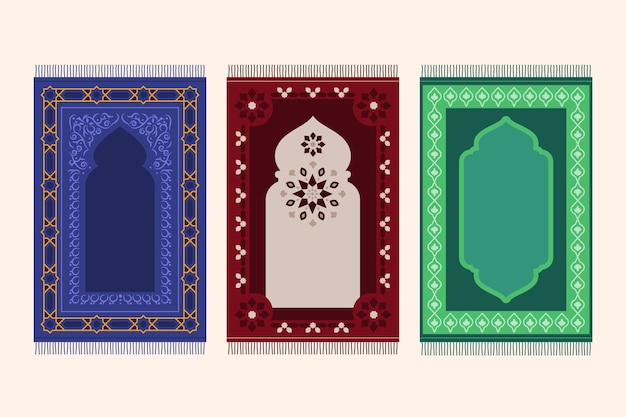
\includegraphics[width=1.26518in,height=2.06178in]{media/image1.jpeg} T
\_A\_ P \_E\_ T \_E\_

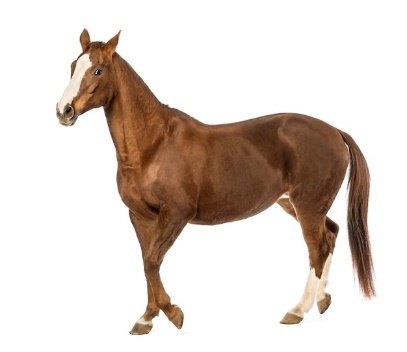
\includegraphics[width=1.85417in,height=1.60240in]{media/image2.jpeg}

C \_\_A\_ V \_\_A\_ L \_\_O\_


\includegraphics[width=1.57292in,height=1.57292in]{media/image3.jpeg}\_E\_\_
STR\_\_E\_\_ L\_\_A\_

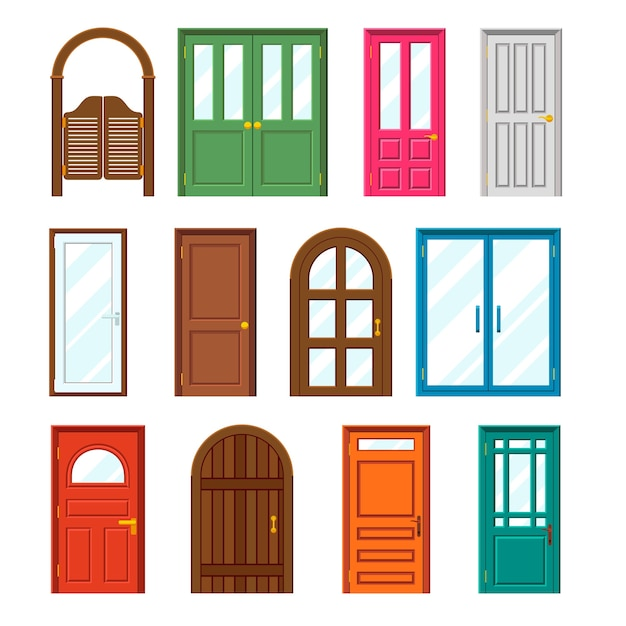
\includegraphics[width=1.27083in,height=1.80035in]{media/image4.jpeg}
P\_O\_\_RT \_\_A\_

%https://www.freepik.com/free-vector/hand-drawn-flat-design-prayer-mat-illustration\_22870006.htm\#page=2\&query=TAPETE\&position=0\&from\_view=search\&track=sph
%\url{https://www.freepik.com/premium-photo/horse-walking-front-white-background_19983860.htm?query=CAVALO\#from_view=detail_alsolike}
%\url{https://www.freepik.com/free-vector/golden-star-3d_830718.htm\#query=ESTRELA\&position=16\&from_view=search\&track=sph}
%https://www.freepik.com/free-vector/set-front-buildings-doors-flat-style\_11053573.htm\#query=PORTA\&position=12\&from\_view=search\&track=sph

Você completou as palavras com

\begin{boxlist}
\boxitem[] Vogais 

\boxitem[] Consoantes
\end{boxlist}

\coment{Apresente as vogais em cartaz. Pergunte o nome dos objetos 
representados nas imagens e, em seguida, convide as crianças para
montar as palavras no alfabeto móvel para identificar as letras faltantes.}

\num{2} Complete o alfabeto com as letras que estão faltado.

\begin{longtable}[]{@{}llllllll@{}}
\toprule
\textbf{A } & \textbf{B} & \textbf{C} & \textbf{D} & \textbf{E} &
\textbf{F} & \textbf{G} & H\tabularnewline
\midrule
\endhead
\textbf{I} & \textbf{J} & \textbf{K} & \textbf{L} & \textbf{M} &
\textbf{N} & \textbf{O} & P\tabularnewline
\textbf{Q} & \textbf{R} & \textbf{S} & \textbf{T} & \textbf{U} &
\textbf{V} & \textbf{W} & X\tabularnewline
\textbf{Y} & \textbf{Z}\tabularnewline
\bottomrule
\end{longtable}

Você completou as palavras com:

\begin{boxlist}
\boxitem[] Vogais 

\boxitem[] Consoantes
\end{boxlist}

\comente{Leve o alfabeto móvel para sala e convide os alunos para
organizar as letras na ordem certa. Em seguida, oriente-os a preencher
o quadro; depois ajude a separar vogais e consoantes.}

\num{3} Leia o poema.

\textbf{A vaca Filomena e a formiga Violeta}\\
Isabel Cristina Silveira Soares

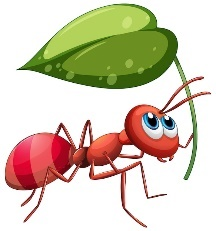
\includegraphics[width=0.97986in,height=1.05208in]{media/image5.jpeg}
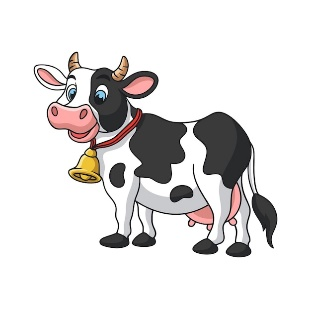
\includegraphics[width=1.16127in,height=0.95833in]{media/image6.jpeg}

\begin{verse}
A vaca Filomena\\
mora na vila formosa\\
A formiga Violeta\\
mora na cerca cor de rosa.

A vaca Filomena\\
come as uvas da parreira\\
A formiga Violeta\\
acha isto uma besteira.
\end{verse}

\fonte{https://seceducacao.padua.rj.gov.br/wp-content/uploads/2021/05/3o-ano-Ling.-Portuguesa-ATIV.17.pdf.
Acesso 28 de Fev 2023.}

Encontre e pinte no texto todas as palavras iniciadas com F e V. 
Depois escreva abaixo as palavras que encontrou.

\reduline{As palavras encontradas são as seguintes: vaca, Filomena, vila,
formosa, formiga, violeta.
Leve as palavras \textit{vaca} e \textit{formiga} em uma caixinha e
apresente-as para as crianças. Faça a leitura das palavras e estimule 
questionamentos sobre esses animais: os alunos sabem como eles são?
Onde esses animais vivem? Que sons eles emitem? Faça com os
alunos a leitura do poema e oriente a localização das palavras iniciadas
com as consoantes V e F.\hfill}

\num{4} Complete os espaços a seguir com as letras iniciais das palavras
\textit{violeta} e \textit{filomena}.

\coment{Leve as palavras Violeta e Filomena em um cartaz. Explore a 
letra inicial e o som da letra nas palavras.}


\includegraphics[width=1.01042in,height=1.55278in]{media/image7.jpeg}

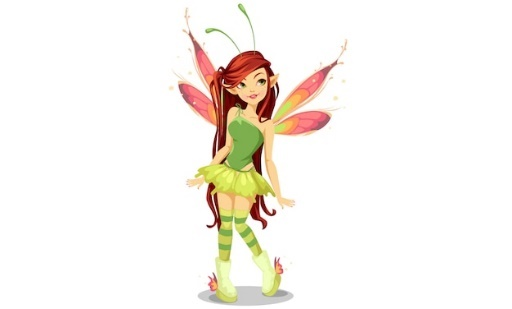
\includegraphics[width=0.87500in,height=1.40486in]{media/image8.jpeg}

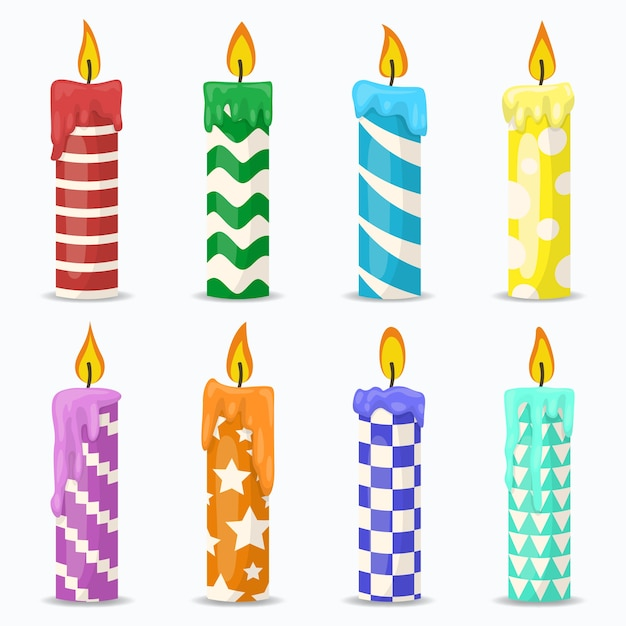
\includegraphics[width=0.56250in,height=1.32083in]{media/image9.jpeg}

\_\_V\_ELA \_FADA \_F\_ACA

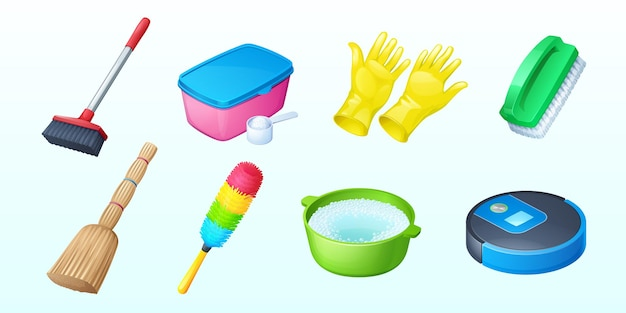
\includegraphics[width=1.12500in,height=1.48958in]{media/image10.jpeg}
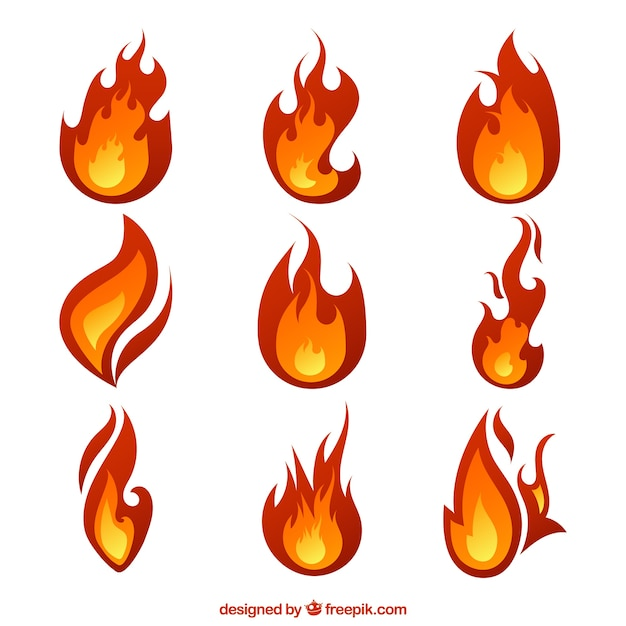
\includegraphics[width=1.34375in,height=1.77083in]{media/image11.jpeg}
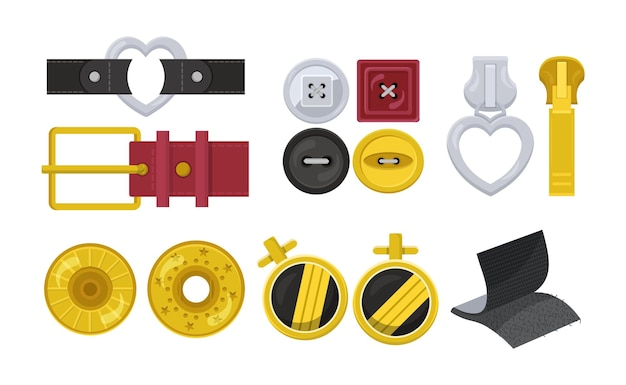
\includegraphics[width=1.77847in,height=0.76369in]{media/image12.jpeg}

\_\_\_F\_\_IVELA \_\_F\_\_OGO VASSOURA

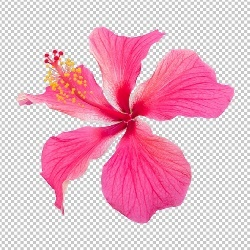
\includegraphics[width=1.13542in,height=1.13542in]{media/image13.jpeg}

\includegraphics[width=1.24653in,height=1.22917in]{media/image14.jpeg}
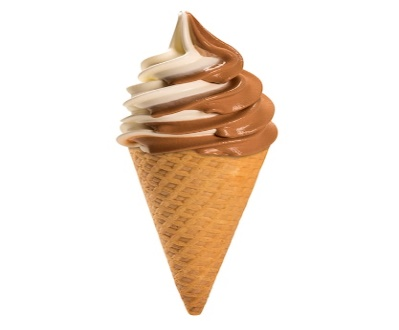
\includegraphics[width=1.00000in,height=1.49583in]{media/image15.jpeg}

SOR\_V\_ETE \_F\_\_OGUETE \_F \_LOR

%\url{https://www.freepik.com/free-vector/collection-christmas-candle-flat-design_6074662.htm\#page=2\&query=VELA\&position=28\&from_view=search\&track=sph}
%\url{https://www.freepik.com/search?format=search\&query=FADA}
%\url{https://www.freepik.com/premium-psd/3d-knife-icon-render-isolated_20395607.htm\#page=4\&query=FACA\&position=17\&from_view=search\&track=sph}
%\url{https://www.freepik.com/free-vector/clasps-design-elements-set-isolated-white-carabiner-hook-snap-bag-belt-buckle-leather-tabs-straps-cufflinks-buttons-different-shapes-materials_27398885.htm\#query=FIVELA\&position=23\&from_view=search\&track=sph}
%https://www.freepik.com/free-vector/great-flames-with-different-designs\_1086041.htm\#query=FOGO\&position=21\&from\_view=search\&track=sph
%\url{https://www.freepik.com/free-vector/cleaning-icons-with-broom-vacuum-cleaner_16956931.htm\#page=2\&query=VASSOURA\&position=7\&from_view=search\&track=sph}
%\url{https://www.freepik.com/premium-photo/vanilla-chocolate-soft-ice-cream-waffled-cone_9043953.htm\#page=3\&query=SORVETE\&position=24\&from_view=search\&track=sph}
%\url{https://www.freepik.com/free-vector/modern-space-rocket-with-realistic-design_2825905.htm\#query=FOGUETE\&position=32\&from_view=search\&track=sph}
%https://www.freepik.com/premium-psd/pink-hibiscus-flower-isolated-rendering\_15458965.htm?query=FLOR\#from\_view=detail\_alsolike

\num{5} Pinte as iniciais de cada palavra.

\coment{Leve para sala palavras iniciadas pelas letras T, D, F, V, B, P. 
Convide as crianças para fazer a leitura, identificado o som das letras
iniciais e finais, e quantidade de sílabas. Também é possível trabalhar
a função social da escrita das palavras}.

\begin{tabular}{|c|c|c|c|c|}
\hline
\textbf{VACINA} & F & T & D & V \\ \hline
\textbf{TESOURA} & P & D & T & F \\ \hline
\textbf{VASSOURA} & B & T & V & F \\ \hline
\textbf{FACA} & V & F & D & T \\ \hline
\textbf{DEDO} & T & V & F & D \\ \hline
\textbf{PANELA} & V & T & P & B \\ \hline
\textbf{DOMINÓ} & B & D & T & P \\ \hline
\textbf{BONECA} & F & P & B & D \\ \hline
\end{tabular}

\num{6} Numere os desenhos conforme os números das palavras.

\coment{Faça leitura das palavras com as crianças, de modo que elas
identifiquem a numeração e façam a associação correta.}

\begin{longtable}[]{@{}llll@{}}
\toprule
\begin{minipage}[b]{0.24\columnwidth}\raggedright\strut
\textbf{1- BOLA}

\textbf{2- FOCA}

\textbf{3- TATU}

\textbf{4- PANELA}

\textbf{5- TAPETE}\strut
\end{minipage} & \begin{minipage}[b]{0.24\columnwidth}\raggedright\strut
\textbf{6- FORMIGA}

\textbf{7- DADO}

\textbf{8- VACA}

\textbf{9- PATO}

\textbf{10- BONECA}\strut
\end{minipage}\tabularnewline
\midrule
\endhead
\textbf{\_\_10\_-} &

\includegraphics[width=1.16667in,height=0.96319in]{media/image16.jpeg} &
\textbf{\_\_8\_\_} &
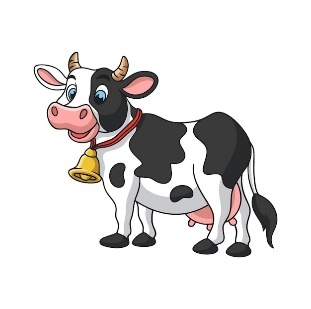
\includegraphics[width=1.16127in,height=0.95833in]{media/image17.jpeg}\tabularnewline
\textbf{\_\_\_2\_} &
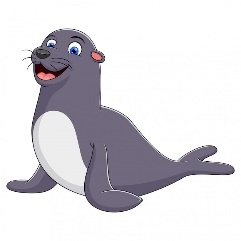
\includegraphics[width=1.09375in,height=1.09375in]{media/image18.jpeg} &
\textbf{\_\_4\_\_} &
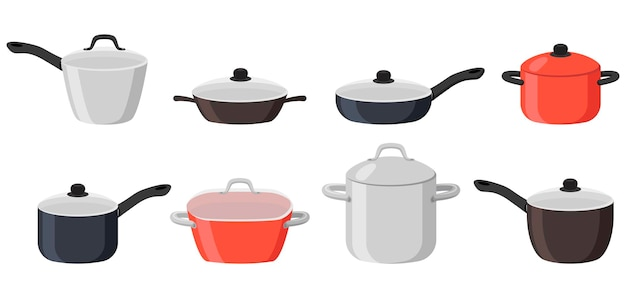
\includegraphics[width=1.27986in,height=0.98958in]{media/image19.jpeg}\tabularnewline
\textbf{\_\_T\_\_} &
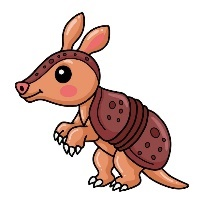
\includegraphics[width=0.92708in,height=0.92708in]{media/image20.jpeg} &
\textbf{\_\_F\_\_} &
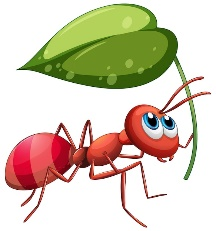
\includegraphics[width=0.97986in,height=1.05208in]{media/image21.jpeg}\tabularnewline
\textbf{\_\_\_B\_} &
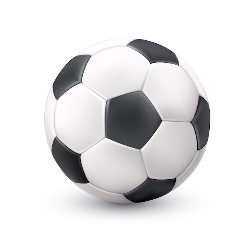
\includegraphics[width=1.13542in,height=1.13542in]{media/image22.jpeg} &
\textbf{\_D\_\_\_} &
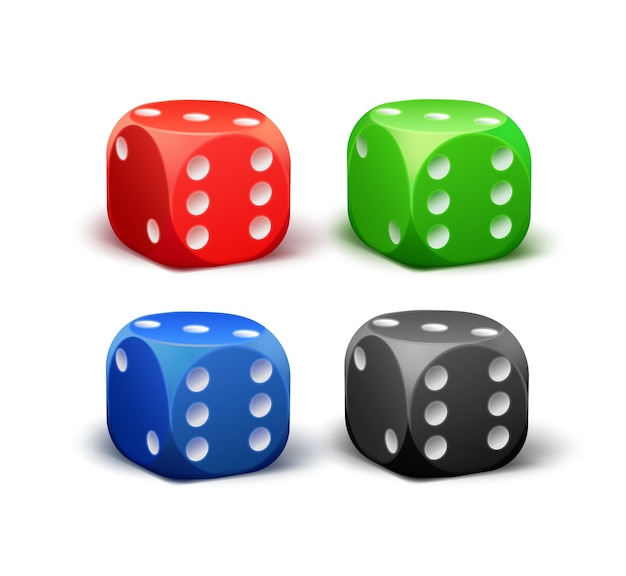
\includegraphics[width=1.23958in,height=1.15833in]{media/image23.jpeg}\tabularnewline
\textbf{\_\_\_P\_} &
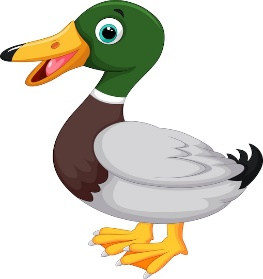
\includegraphics[width=1.19722in,height=1.27083in]{media/image24.jpeg} &
\textbf{\_\_T\_\_} &
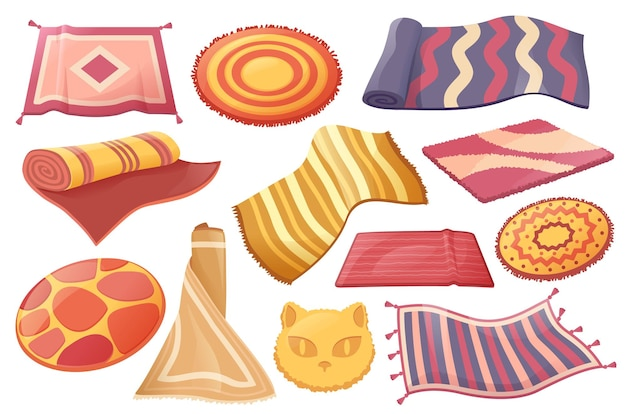
\includegraphics[width=2.21875in,height=1.11458in]{media/image25.jpeg}\tabularnewline
\bottomrule
\end{longtable}

%https://www.freepik.com/premium-vector/pink-chibi-girl\_9687656.htm\#query=BONECA\&position=34\&from\_view=search\&track=sph
%\url{https://www.freepik.com/premium-vector/cartoon-illustration-cool-cow_17447402.htm\#page=2\&query=VACA\&position=48\&from_view=search\&track=sph}
%https://www.freepik.com/premium-vector/seal-cartoon-isolated\_6122224.htm\#query=FOCA\&position=36\&from\_view=search\&track=sph
%\url{https://www.freepik.com/free-vector/frying-pans-saucepans-cartoon-illustration-set-metal-cooking-pots-with-lid-different-sizes-stainless-utensils-making-soup-boiling-water-household-kitchen-concept_26921753.htm\#query=PANELA\&position=1\&from_view=search\&track=sph}
%https://www.freepik.com/premium-vector/cute-little-armadillo-cartoon-standing\_27006356.htm\#query=TATU\&position=13\&from\_view=search\&track=sph
%\url{https://www.freepik.com/free-vector/ant-holding-green-leaf_19589093.htm\#query=FORMIGA\&position=4\&from_view=search\&track=sph}
%\url{https://www.freepik.com/premium-vector/cartoon-wool-carpets-bath-rug-woven-mat-carpet-roll-home-floor-textile-decor-vector-illustration-set_28995572.htm\#page=2\&query=TAPETE\&position=43\&from_view=search\&track=sph}
%\url{https://www.freepik.com/premium-vector/cute-cartoon-duck_3219176.htm\#query=PATO\&position=8\&from_view=search\&track=sph}
%https://www.freepik.com/free-vector/soccer-ball-realistic-white-black-picture\_2875610.htm\#query=bola\&position=1\&from\_view=search\&track=sph

\num{7} Complete as palvaras com \textbf{-ca -co -cu} ou \textbf{-qua -que -qui}.

\coment{Convide as crianças a falar o nome das imagens para identificar a grafia da palavra.}


\includegraphics[width=1.30278in,height=0.81667in]{media/image26.jpeg}
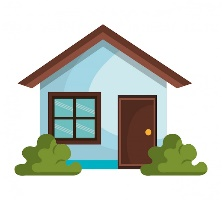
\includegraphics[width=1.00903in,height=0.90972in]{media/image27.jpeg}

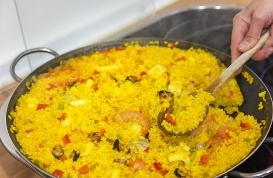
\includegraphics[width=1.24028in,height=0.81042in]{media/image28.jpeg}
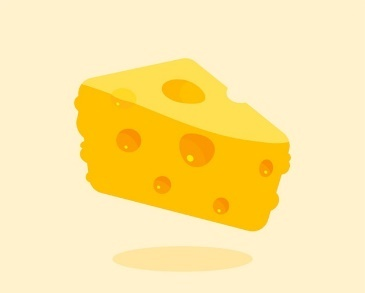
\includegraphics[width=1.05556in,height=0.81667in]{media/image29.jpeg}

CASA QUEI\_\_\_\_\_IJO CU \_\_\_\_\_\_\_SCUS CU\_TIA

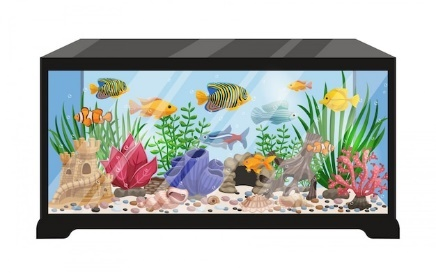
\includegraphics[width=1.98343in,height=1.24038in]{media/image30.jpeg}
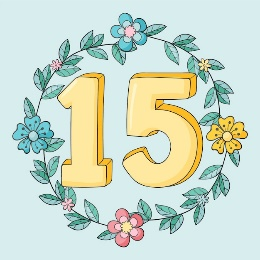
\includegraphics[width=1.18269in,height=1.18269in]{media/image31.jpeg}

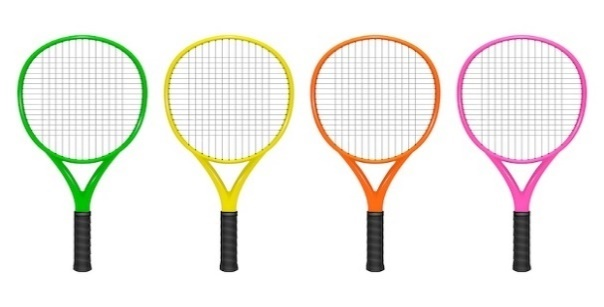
\includegraphics[width=0.70192in,height=1.39623in]{media/image32.jpeg}

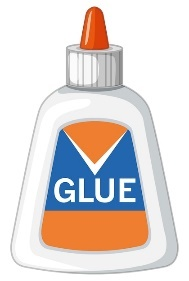
\includegraphics[width=0.85819in,height=1.27885in]{media/image33.jpeg}

QUI\_\_\_NZE Á \_\_QUA\_\_RIO CO\_\_\_LA RA\_QUE\_TE

%https://www.freepik.com/free-vector/beautiful-home\_4979878.htm\#query=CASA\&position=27\&from\_view=search\&track=sph
%https://www.freepik.com/free-vector/cheese-isolated-cartoon-art-illustration\_14478854.htm\#query=QUEIJO\&position=3\&from\_view=search\&track=sph
%https://www.flickr.com/photos/gjshepherd/18994508411
%https://www.freepik.com/free-vector/hand-drawn-15th-anniversary-birthday\_22751030.htm\#query=N\%C3\%9AMERO\%2015\&position=6\&from\_view=search\&track=ais
%https://www.freepik.com/free-vector/aquarium-tank-cartoon-illustration\_5971410.htm\#query=AQUARIO\&position=34\&from\_view=search\&track=sph
%https://www.freepik.com/free-vector/bottle-latex-glue\_19589095.htm\#query=COLA\&position=0\&from\_view=search\&track=sph

\num{8} Encontre a sílaba mais forte e complete com O ou U.

\coment{Leve para a classe uma caixinha enfeitada com palavras terminadas
com O e U. Passe a caixinha para os alunos em círculo, ao som de uma 
música. Quando a música parar, o aluno que estiver com a caixinha na 
mão deve ler a palavra observando a letra  final. Em seguida, convide
toda a turma a pronunciar a palavra e, então, descobrir a sílaba forte.
Explique como descobrir quando a sílaba é forte e fraca, ensinando que,
quando o U está no final, ele é sempre forte, e que o O é sempre fraco
no final das palavras.}

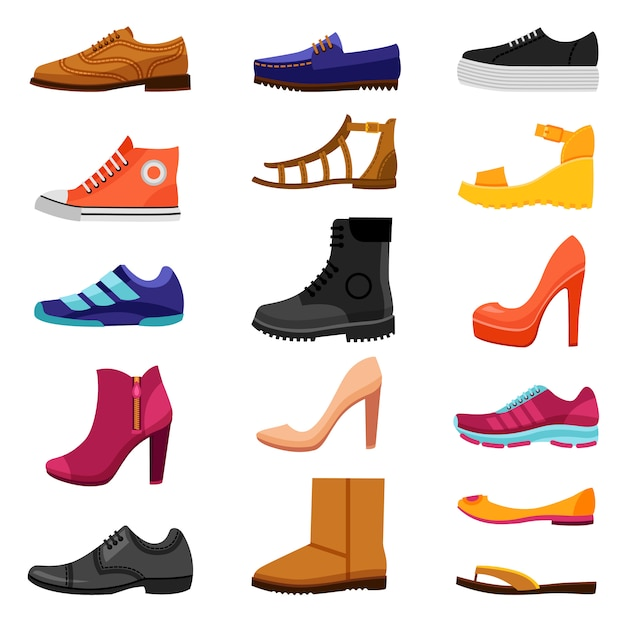
\includegraphics[width=1.65486in,height=0.74499in]{media/image34.jpeg}
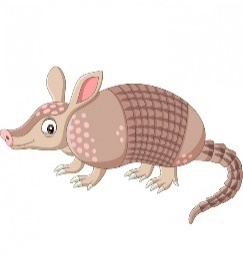
\includegraphics[width=1.09512in,height=0.74522in]{media/image35.jpeg}
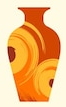
\includegraphics[width=0.69978in,height=1.10152in]{media/image36.jpeg}

TAT\_\_U\_\_ VAS\_O\_\_ SAPAT\_\_O\_\_


\includegraphics[width=0.59861in,height=1.03542in]{media/image37.jpeg}

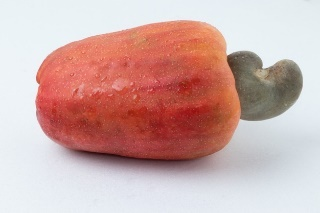
\includegraphics[width=1.26250in,height=0.68750in]{media/image38.jpeg}
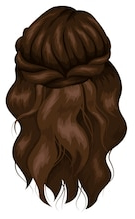
\includegraphics[width=0.59873in,height=0.93296in]{media/image39.jpeg}

CABEL\_\_O\_ CAJ\_\_U\_\_ ESPELH\_O\_\_

%https://www.freepik.com/premium-vector/cartoon-armadillo-white\_6408471.htm\#query=TATU\&position=27\&from\_view=search\&track=sph
%\url{https://www.freepik.com/premium-photo/fresh-cashew-isolated-white-background_18591010.htm\#page=6\&query=CAJU\&position=5\&from_view=search\&track=sph}
%\url{https://www.freepik.com/free-vector/contemporary-ceramic-vases-modern-jugs-pots_29836873.htm\#query=VASO\&position=21\&from_view=search\&track=sph}
%\url{https://www.freepik.com/free-vector/women-wigs-hairstyle-realistic-icons-set_4016983.htm\#page=3\&query=CABELO\&position=49\&from_view=search\&track=sph}
%\url{https://www.freepik.com/free-vector/footwear-colored-icons-set_4431156.htm\#query=SAPATO\&position=1\&from_view=search\&track=sph}
%https://www.freepik.com/free-vector/sticker-template-pink-mirror-with-handle-isolated\_20721062.htm\#query=ESPELHO\&position=12\&from\_view=search\&track=sph

\num{9} Pinte as palvras escritas com C que tem o som de S.
%Felipe: aqui precisamos padronizar, como comentei anteriormente. 

\coment{Leve para sala palavras escritas com C. Organize uma roda de
conversa na qual você orientará os alunos a organizar as palavras de
acordo com a vogal que acompanha a letra C. Em seguida, explique a 
regra para descobrir se o C tem som de K ou S.}

\begin{longtable}[]{@{}lllll@{}}
\toprule
\textbf{CINEMA} & \textbf{CASA} & \textbf{CISNE} & \textbf{CEGO} &
\textbf{COCADA}\tabularnewline
\midrule
\endhead
\textbf{CADEIRA} & \textbf{CARRO} & \textbf{CINTO } & \textbf{COCO} &
\textbf{CAMA}\tabularnewline
\bottomrule
\end{longtable}

\num{10} Troque as letras e forme outras palavras.

\coment{Utilize o alfabeto móvel com as palavras
solicitadas no exercício e outras. Também é possível fazer a 
brincadeira da forca.}

\begin{longtable}[]{@{}lll@{}}
\toprule
\textbf{V POR F} & \textbf{D POR T} & \textbf{B POR P}\tabularnewline
\midrule
\endhead
\textbf{VACA} & \textbf{DADO} & \textbf{BODE}\tabularnewline
\textbf{\_F\_ACA} & \textbf{TATO} & \textbf{\_\_P\_ODE}\tabularnewline
\textbf{VILA} & \textbf{DIA} & \textbf{BOTE}\tabularnewline
\textbf{\_F\_I LA} & \textbf{\_T\_IA} & \textbf{\_P\_OTE}\tabularnewline
\bottomrule
\end{longtable}

\num{11} Complete a cruzadinha com o nome das figuras.

\coment{Explore as frutas e legumes da atividade, fazendo 
questionamentos. Monte as palavras no alfabeto móvel com as crianças.
Em seguida, oriente a escrita na cruzadinha.}

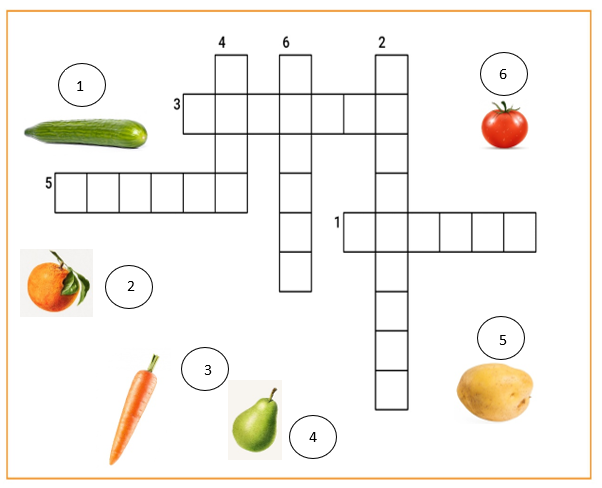
\includegraphics[width=5.69167in,height=4.10139in]{media/image40.png}

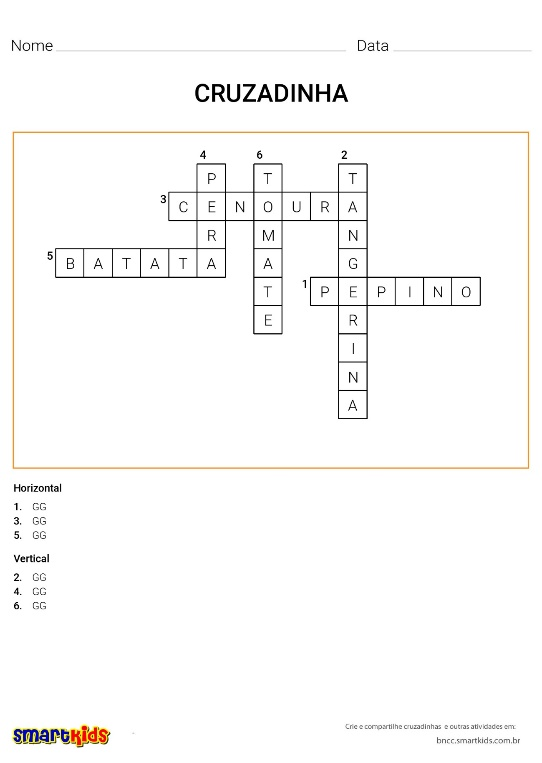
\includegraphics[width=2.40385in,height=1.79075in]{media/image41.jpeg}

Resposta da cruzadinha

%\url{https://www.freepik.com/free-photo/green-cucumber_7399055.htm?query=PEPINO\#from_view=detail_alsolike}
%\url{https://www.freepik.com/free-vector/hand-drawn-natural-fresh-oranges-set_16351577.htm\#query=tangerina\&position=44\&from_view=search\&track=sph}
%\url{https://www.freepik.com/premium-photo/fresh-carrot-isolated-white_9544212.htm\#page=2\&query=CENOURA\&position=16\&from_view=search\&track=sph}
%\url{https://www.freepik.com/free-vector/vintage-pear-illustration_16279755.htm\#query=PERA\&position=1\&from_view=search\&track=sph}
%\url{https://www.freepik.com/free-photo/potato_1025630.htm\#query=BATATA\&position=2\&from_view=search\&track=sph}
%https://www.freepik.com/free-vector/fresh-tomato\_957857.htm\#query=TOMATE\&position=17\&from\_view=search\&track=sph

\num{12} Encontre e pinte as palavras no diagrama.

\coment{Depois da leitura das palavras, oriente os alunos a localizá-las
no diagrama.}

\begin{longtable}[]{@{}llllllll@{}}
\toprule
TATU- CABELO - BONECA- PANELA- CAJU - FADA- DADO - VASO -- CAMA --
TAPETE\tabularnewline
\midrule
\endhead
D & B & F & A & D & A & D & G\tabularnewline
A & C & A & B & E & L & O & U\tabularnewline
G & Y & B & O & C & A & M & A\tabularnewline
S & T & I & N & H & M & A & Q\tabularnewline
P & A & N & E & L & A & D & F\tabularnewline
H & T & O & C & A & J & U & L\tabularnewline
J & U & K & A & D & A & D & O\tabularnewline
T & A & P & E & T & E & Z & X\tabularnewline
K & V & A & S & O & B & G & J\tabularnewline
\bottomrule
\end{longtable}

\colorsec{Treino}

\num{1} Observe o animal que Júlia encontrou enquanto brincava na 
fazenda do Tio Belo.


\includegraphics[width=1.36528in,height=1.64861in]{media/image42.jpeg}

%\url{https://www.freepik.com/premium-vector/set-ants-carry-leaf-stone-tree-branches-white_9221745.htm?query=formiga\#from_view=detail_alsolike}
%Acesso 01 Mar 2023.

A palavra que começa com a mesma letra do nome do animal que Júlia
encontrou é

\begin{minipage}{.5\textwidth}
\begin{escolha}
\item vaso.

\item gato.

\item bola.

\item foca
\end{escolha}
\end{minipage}
\sidetext{SAEB: Relacionar elementos sonoros das palavras com sua
representação escrita

BNCC: EF02LP03 -- Ler e escrever palavras com correspondências
regulares diretas entre letras e fonemas (f, v, t, d, p, b) e
correspondências regulares contextuais (c e q; e e o, em posição átona
em final de palavra).}

a) Incorreta. O animal encontrado por Júlia é uma \textit{formiga}, 
que começa com a letra F, não com a letra V.
b) Incorreta. O animal encontrado por Júlia é uma \textit{formiga}, 
que começa com a letra F, não com a letra G.
c) Incorreta. O animal encontrado por Júlia é uma \textit{formiga}, 
que começa com a letra F, não com a letra B. 
d) Correta. Tanto \textit{formiga} quanto \textit{foca} são palavras
que começam com a letra F.

\num{2} Observe a palavra que Tiago leu para sua professora.

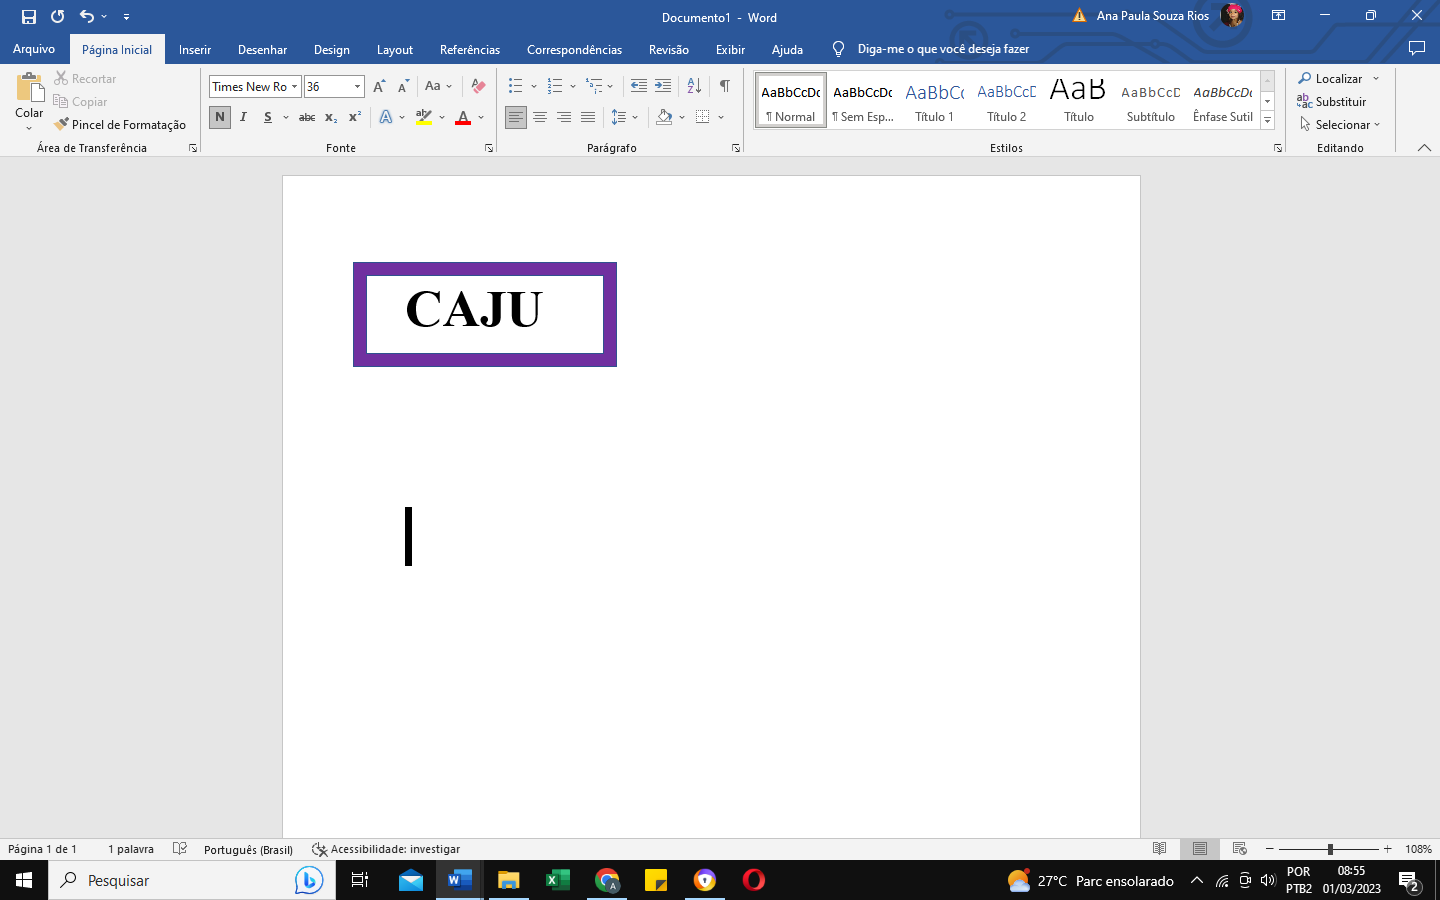
\includegraphics[width=2.79792in,height=1.15833in]{media/image43.png}

O nome da figura que termina com a mesma letra da palavra que Tiago leu é

\begin{escolha}
\item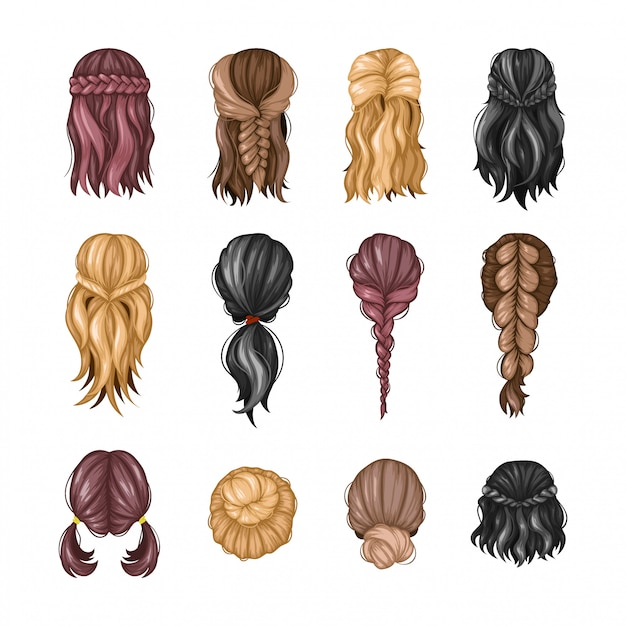
\includegraphics[width=0.79792in,height=0.81667in]{media/image44.jpeg}

\item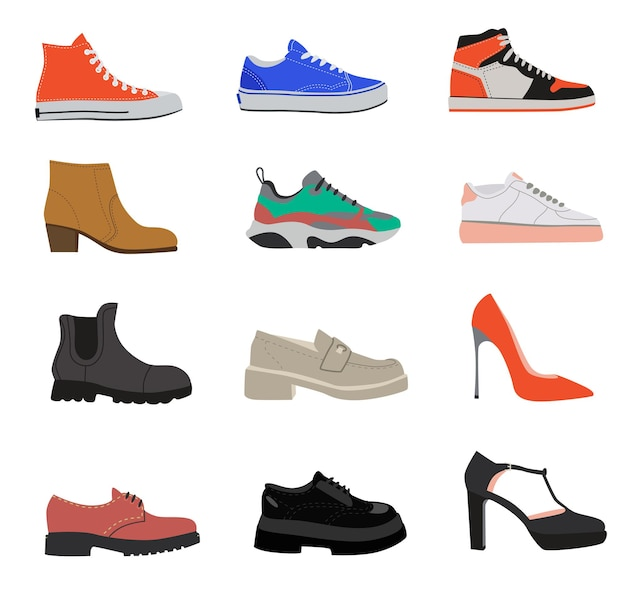
\includegraphics[width=1.02847in,height=0.72292in]{media/image45.jpeg}

\item
\includegraphics[width=0.79792in,height=0.79931in]{media/image46.jpeg}

\item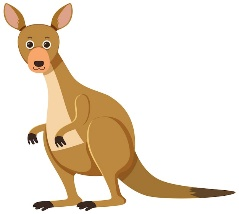
\includegraphics[width=1.08611in,height=0.97222in]{media/image47.jpeg}
\end{escolha}

\coment{SAEB: Relacionar elementos sonoros das palavras com sua
representação escrita

BNCC: EF02LP03 -- Ler e escrever palavras com correspondências
regulares diretas entre letras e fonemas (f, v, t, d, p, b) e
correspondências regulares contextuais (c e q; e e o, em posição átona
em final de palavra).}

a) Incorreta. \textit{Caju} termina com a letra U, mas \textit{cabelo} termina com a letra O.

b) Incorreta. \textit{Caju} termina com a letra U, mas \textit{sapato} termina com a letra O.

c) Incorreta. \textit{Caju} termina com a letra U, mas \textit{relógio} termina com a letra O.

(D) Correta. As palavras \textit{caju} e \textit{canguru} terminam com a letra U.

%\url{https://www.freepik.com/premium-vector/set-variety-women-hairstyles_7719339.htm\#from_view=detail_alsolike}
%\url{https://www.freepik.com/free-vector/random-female-shoes-flat-illustrations-set-summer-autumn-winter-foot-wear-women-moccasins-boots-trainers-heels-isolated-white_20827876.htm\#query=SAPATO\&position=1\&from_view=search\&track=sph}
%\url{https://www.freepik.com/free-vector/round-wall-quartz-clock-red-color-isolated-white-background_13031909.htm\#query=RELOGIO\&position=27\&from_view=search\&track=sph}
%https://www.freepik.com/free-vector/kangaroo-cartoon-character-isolated\_29098402.htm\#query=CANGURU\&position=7\&from\_view=search\&track=sph

\num{3} Observe o presente que Bruna ganhou.

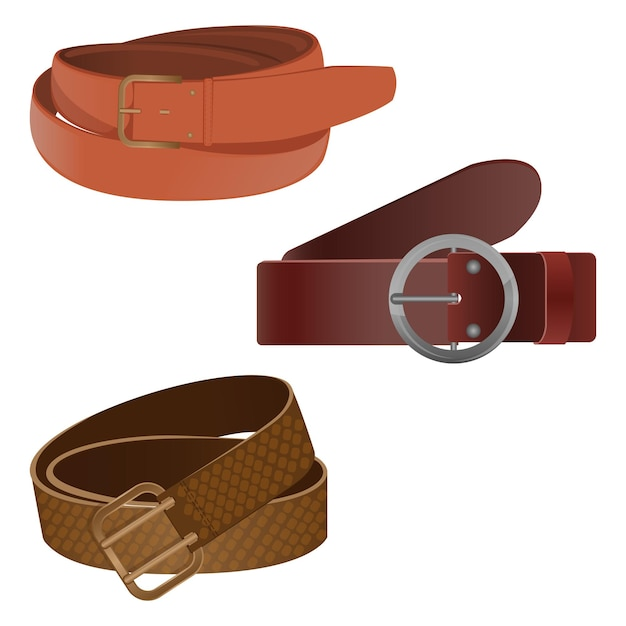
\includegraphics[width=3.62413in,height=2.01875in]{media/image48.jpeg}

%\url{https://www.freepik.com/premium-vector/set-leather-waist-belts-isolated-background_13798858.htm\#query=CINTO\&position=38\&from_view=search\&track=sph}
%Acesso 01 Mar 2023.

A palavra que começa como o mesmo som da letra do nome do presente de Bruna é

\begin{minipage}{.5\textwidth}
\begin{escolha}
\item cama.

\item cubo.

\item cebola.

\item cocada.
\end{escolha}
\end{minipage}
\sidetext{SAEB: Relacionar elementos sonoros das palavras com sua
representação escrita.

BNCC: EF02LP03 -- Ler e
escrever palavras com correspondências regulares diretas entre letras e
fonemas (f, v, t, d, p, b) e correspondências regulares contextuais (c e
q; e e o, em posição átona em final de palavra).}

a) Incorreta. A letra C da palavra \textit{Cinto} tem som de S, mas,
na palavra \textit{cama}, essa letra tem som de K. 
b) Incorreta. A letra C da palavra \textit{Cinto} tem som de S, mas,
na palavra \textit{cubo}, essa letra tem som de K.
c) Correta. A letra C das palavras \textit{Cinto} e \textit{cebola}
têm som de S.
d) Incorreta. A letra C da palavra \textit{Cinto} tem som de S, mas,
na palavra \textit{cocada}, essa letra tem som de K.

\chapter{Lendo e escrevendo}
\markboth{Módulo 2}{}

\coment{Habilidades da BNCC: EF02LP04, EF02LP05}

\colorsec{Habilidades do SAEB}

\begin{itemize}
\item Ler palavras.
\item Escrever palavras.
\item Ler frases.
\end{itemize}

\conteudo{Para escrever uma palavra, você precisa usar as letras que
são chamadas de vogais e as consoantes.

%Paulo: é o caso de, na explicação abaixo, colocar as vogais e consoantes em destaque, dentro de um box, em fonte grande e caixa alta 

As vogais são \textbf{A -- E -- I -- O -- U} 

e as consoantes são \textbf{B -- C -- D -- F -- G -- H -- J -- K -- L -- M -- N -- P -- Q -- R -- S
-- T -- V -- W -- Y -- X -- Z.}

As palavras são lidas e escritas da esquerda para a direita.

%Paulo, atenção: no original, existe uma seta indicando o sentido da leitura das palavras abaixo

\textbf{GRAVIOLA LÂMPADA AVIÃO LARANJA }

Existem diferentes maneiras de compor a sílaba de uma palavra. 

\textbf{CONSOANTE + VOGAL}: é o que acontece nas três sílabas das 
palavras \textit{sapato} e \textit{telefone}: SA-PA-TO e TE-LE-FO-NE

\textbf{VOGAL}: é o que acontece na segunda sílaba das  
palavras \textit{saída} e \textit{saúde}: SA-Í-DA e SA-Ú-DE

\textbf{CONSOANTE + VOGAL + CONSOANTE}: é o que acontece na 
primera sílaba das palavras \textit{porta} e \textit{cortina}:
POR-TA e COR-TI-NA

\textbf{CONSOANTE + CONSOANTE + VOGAL}: é o que acontece na 
primera sílaba da palavra \textit{criança} e na última
sílaba da palavra \textit{livro}: CRI-AN-ÇA e LI-VRO 

Observe o quadro abaixo, com outros exemplos:

\begin{longtable}[]{@{}lllll@{}}
\toprule
\textbf{PALAVRAS} & \textbf{FORMAÇÃO SILÁBICA CV} & \textbf{FORMAÇÃO
SILÁBICA V} & \textbf{FORMAÇÃO SILÁBICA CVC} & \textbf{FORMAÇÃO SILÁBICA
CCV}\tabularnewline
\midrule
\endhead
\textbf{GRAVIOLA} & GRA- \textbf{VI}- O-\textbf{LA} & GRA- VI-
\textbf{O}-LA & \textbf{*} & \textbf{GRA}- VI- O-LA\tabularnewline
\textbf{LÂMPADA} & LÂM -- \textbf{PA - DA} & * & \textbf{LÂM}--PA - DA &
*\tabularnewline
\textbf{AVIÂO} & A -- \textbf{VI} - ÂO & \textbf{A} -- VI - ÂO & * &
*\tabularnewline
\textbf{LARANJA} & \textbf{LA}-RAN-\textbf{JÁ} & * & LA-\textbf{RAN}-JÁ
& *\tabularnewline
\bottomrule
\end{longtable}

Note que, em todas as formações das sílabas, aparecem vogais. Isso
acontece porque não existe sílaba sem vogal, isto é, uma  sílaba não
se forma só com consoantes.

Observe a frase a seguir:

\textbf{O avião pousou cedo.}

Você conhece esse sinal em cima da letra A da palavra \textbf{avião}?

Esse sinal é o \textbf{til}, usado nas vogais A e O para marcar a
nasalidade presente na sílaba.

As marcas de nasalidade aparece também nas letras M e N, no final da
sílaba. É o que acontece, por exemplo, com as seguintes palavras:

\textbf{LÂMPADA E LARANJA}

A letra \textbf{M} é utilizada antes das consoantes P e B.  
A letra \textbf{N} é usada antes das demais consoantes, nunca 
no final das palavras.
}

\colorsec{Atividades}

\num{1} Escreva os nomes das figuras.

\coment{Leve o alfabeto móvel para a sala de 
aula. Convide as crianças para manusear as letras; em seguida, 
oriente-as a formar as palavras que nomeiam as figuras. Sugira a elas
que, antes de escrever, elas devem pronunciar a palavra, escrevendo-a 
por sílabas ou pedacinhos.}

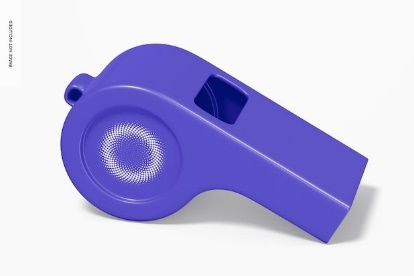
\includegraphics[width=1.46154in,height=0.93603in]{media/image49.jpeg}
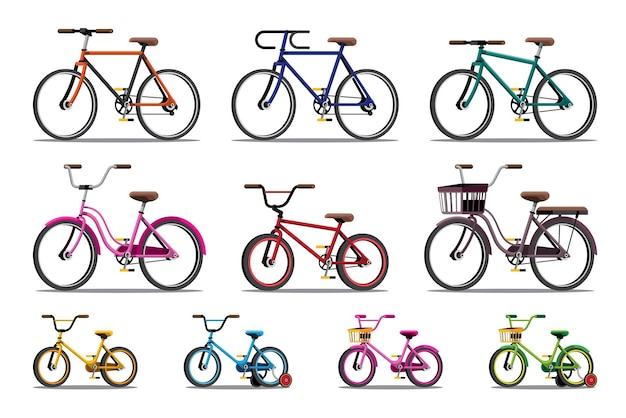
\includegraphics[width=1.16587in,height=0.93269in]{media/image50.jpeg}
\includegraphics[width=1.42308in,height=1.21950in]{media/image51.jpeg}

\reduline{Apito\hfill}

\reduline{Bicicleta\hfill}

\reduline{Árvore\hfill}

\includegraphics[width=1.10833in,height=1.00903in]{media/image52.jpeg}
\includegraphics[width=0.85556in,height=0.92222in]{media/image53.jpeg}
\includegraphics[width=0.79808in,height=0.79808in]{media/image54.jpeg}

\reduline{Bola\hfill}

\reduline{Raposa\hfill}

\reduline{Gaiola\hfill}

\includegraphics[width=0.91319in,height=1.16319in]{media/image55.jpeg}
\includegraphics[width=1.62569in,height=1.25000in]{media/image56.jpeg}
\includegraphics[width=0.93990in,height=1.27885in]{media/image57.jpeg}

\reduline{Pera\hfill}

\reduline{Pedra\hfill}

\reduline{Unha\hfill}

%\url{https://www.freepik.com/premium-psd/plastic-whistle-mockup_13956504.htm\#page=2\&query=apito\&position=33\&from_view=search\&track=sph}
%\url{https://www.freepik.com/free-vector/various-models-styles-bikes-riders-choose-from-according-age-usage-vector-cartoon-illustration-bicycle-isolated-white-background_23248359.htm\#query=bicicleta\&position=41\&from_view=search\&track=sph}
%\url{https://www.freepik.com/free-vector/tree_6132448.htm\#query=arvore\&position=12\&from_view=search\&track=sph}
%\url{https://www.freepik.com/free-vector/vector-isolated-realistic-soccer-ball-white_10601489.htm\#query=bola\&position=5\&from_view=search\&track=sph}
%\url{https://www.freepik.com/free-vector/hand-drawn-fox-collection_9468869.htm\#page=2\&query=raposa\&position=4\&from_view=search\&track=sph}
%\url{https://www.freepik.com/premium-photo/close-up-guava-fruit-pink-fresh-organic-with-leaves-whole-sliced-isolated-white-background-front-view_3766358.htm\#query=graviola\&position=33\&from_view=search\&track=sph}
%\url{https://www.freepik.com/free-vector/stones-rocks-cartoon_13050167.htm\#query=pedra\&position=11\&from_view=search\&track=sph}
%https://www.freepik.com/free-vector/illustration-nails-with-nail-polish-without-nail-polish\_11053390.htm\#query=unha\&position=11\&from\_view=search\&track=sph

\num{2} Separe as sílabas das palavras, depois circule as sílabas formadas por
consoante + consoante + vogal.

\coment{Leia as palavras com os alunos, 
orientando-os a identificar vogais e consoantes. Também é possível 
montar algumas palavras com o alfabeto móvel. Em seguida, peça a eles 
que batam palmas cada vez que um pedacinho da palavra for pronunciado.}

\begin{longtable}[]{@{}ll@{}}
\toprule
\textbf{PRATO} & Pra - to\tabularnewline
\midrule
\endhead
\textbf{FORMIGA} & For- mi -ga\tabularnewline
\textbf{BRAÇO} & Bra -ço\tabularnewline
\textbf{DRAGÃO} & Dra- gão\tabularnewline
\textbf{CRAVO} & Cra -- vo\tabularnewline
\bottomrule
\end{longtable}

\num{3} Ligue as palavras com seu desenho.

\coment{Leve para sala as palavras dentro de uma sacola. Cada criança
deve pegar uma palavra da sacola para fazer a leitura. Depois proponha
a atividade.}

Bicicleta

\includegraphics[width=0.38403in,height=0.53889in]{media/image59.png}

Janela

\includegraphics[width=0.60069in,height=0.48056in]{media/image60.png}

Borboleta

\includegraphics[width=0.49028in,height=0.40833in]{media/image61.png}

Dragão

\includegraphics[width=0.74931in,height=0.52292in]{media/image62.png}

Avião

\includegraphics[width=0.68542in,height=0.66319in]{media/image63.png}

\includegraphics[width=0.53403in,height=0.56667in]{media/image64.jpeg}

Prego

\includegraphics[width=0.91319in,height=0.52292in]{media/image65.png}

PIÃO

\includegraphics[width=0.65385in,height=0.73262in]{media/image66.png}

MANGA

Pomba

%\url{https://www.freepik.com/free-vector/various-models-styles-bikes-riders-choose-from-according-age-usage-vector-cartoon-illustration-bicycle-isolated-white-background_23248359.htm\#query=BICICLETA\&position=44\&from_view=search\&track=sph}
%\url{https://www.freepik.com/free-vector/hand-drawn-dove-outline-illustration_22340867.htm\#query=pomba\&position=1\&from_view=search\&track=sph}
%\url{https://www.freepik.com/free-photo/mango-table_6901195.htm\#query=manga\&position=1\&from_view=search\&track=sph}
%\url{https://www.freepik.com/free-vector/butterfly-collection_3980202.htm\#query=borboleta\&position=19\&from_view=search\&track=sph}
%\url{https://www.freepik.com/free-vector/different-kind-dinosaurs_22717262.htm\#query=dinossauro\&position=4\&from_view=search\&track=sph}
%\url{https://www.freepik.com/free-vector/wooden-windows-with-open-shutters-mediterranean-style-white_12569303.htm\#query=janela\&position=34\&from_view=search\&track=sph}
%\url{https://www.freepik.com/free-vector/air-transportation-set_4559015.htm\#query=avi\%C3\%A3o\&position=4\&from_view=search\&track=sph}
%\url{https://www.freepik.com/free-vector/frying-pans-saucepans-cartoon-illustration-set-metal-cooking-pots-with-lid-different-sizes-stainless-utensils-making-soup-boiling-water-household-kitchen-concept_26921753.htm\#query=panela\&position=0\&from_view=search\&track=sph}
%\url{https://www.freepik.com/free-vector/screw-sticker-white-background_17622561.htm\#query=prego\&position=23\&from_view=search\&track=sph}
%\url{https://www.freepik.com/free-vector/flat-design-christmas-toys-collection_11374313.htm\#query=spinning\%20top\&from_query=pi\%C3\%A3o\&position=2\&from_view=search\&track=sph}
%\url{https://www.freepik.com/free-photo/mango_8171055.htm\#query=manga\&position=9\&from_view=search\&track=sph}

\num{4} Pinto no diagrama as palavras do quadro abaixo.

\coment{Faça a leitura das palavras com os alunos aproveite esse 
momento para trabalhar a função da escrita.}

\begin{longtable}[]{@{}llll@{}}
\toprule
PIÃO & CAMA & LEÂO & PEDRA\tabularnewline
\midrule
\endhead
ABACATE & SAPO & PATO & SABÃO\tabularnewline
TRATOR & GRAMA & CISNE\tabularnewline
\bottomrule
\end{longtable}

\begin{longtable}[]{@{}llllllllll@{}}
\toprule
P & I & Ã & O & D & O & W & E & I & S\tabularnewline
\midrule
\endhead
F & H & P & I & S & A & B & Ã & O & A\tabularnewline
S & J & L & S & J & U & Y & U & J & P\tabularnewline
L & O & A & B & A & C & A & T & E & O\tabularnewline
E & U & I & D & A & S & A & L & K & A\tabularnewline
à & A & B & G & C & A & Y & J & G & P\tabularnewline
O & S & A & P & A & T & O & P & R & E\tabularnewline
Z & D & R & F & D & M & E & C & A & D\tabularnewline
L & T & R & A & T & O & R & Q & M & R\tabularnewline
B & U & G & T & E & Y & E & & A & A\tabularnewline
A & C & I & S & N & E & O & P & U & O\tabularnewline
L & O & L & O & C & A & M & A & A & G\tabularnewline
\bottomrule
\end{longtable}

\coment{R: pião -- cama -- leão- pedra- abacate- sapo- cama- pato -- sabão --
trator -- grama- cisne.}

\num{5} Coloque o til nas palavras sempre que necessário.

\coment{Construa com os alunos critérios para
identificar as marcas de nasalidade de uma palavra. Sugira que leiam
as palavras em voz alta e posicionem os dedos indicador e polegar sobre
o nariz ao pronunciar palavras com esses sons, para perceberem a
diferença, por exemplo, entre a pronúncia de palavras como \textit{lá}
e \textit{lã}, \textit{manha} e \textit{manhã}. Explique que o til
acompanha apenas as vogais A e O.}

IRMÃO -- SALA -- MÃO -- PATO -- MAÇÃ -- VILA -- MOLA -- MANHÃ -- LÃ

\num{6}

Observe a marca de nasalização e complete as palavras com M ou N.

\coment{Siga as orientações da questão anterior, 
aguçando a atenção das crianças quanto à diferença de pronúncia de
palavras como \textit{pote} e \textit{ponte} e \textit{rapa} e 
\textit{rampa}. Reforce a ideia de M sempre antes de B, e N antes de
outras consoantes.}

LÂ\_M\_PADA CA\_\_M\_\_PO LARA\_\_N\_JA TRO\_N\_CO VE\_\_N\_\_TO
PO\_\_BA

U\_M\_\_ BIGO PO\_\_N\_TE RA\_\_M\_PA BO\_M\_BOM TE\_M\_PO PI\_N\_TA

\num{7} Observe as imagens e escreva uma frase para cada uma.

\coment{Explore as imagens com as crianças e oriente a construção 
das frases.}

\includegraphics[width=1.38264in,height=1.28681in]{media/image67.jpeg}

\reduline{Uma resposta possível é \textit{As crianças andam a cavalo}.\hfill}

\includegraphics[width=1.21656in,height=1.16552in]{media/image68.jpeg}

\reduline{Uma resposta possível é \textit{A menina leva flores no carrinho}.\hfill}

%https://www.freepik.com/premium-vector/flowers-little-girl-vector-illustration\_16703215.htm?query=MENINA\#from\_view=detail\_alsolike
%\url{https://www.freepik.com/premium-vector/cartoon-boy-girl-riding-horse_2499886.htm\#query=menina\%20de\%20cavalo\&position=34\&from_view=search\&track=ais}

\num{8}

Leia as frases a seguir e faça um desenho para representar.

\coment{Oriente a leitura das frases explorando com as
crianças o conteúdo de cada uma delas e as diferentes possibilidades
de representação.}

\begin{longtable}[]{@{}l@{}}
\toprule
O CAVALO GOSTA DE CORRER.\tabularnewline
\midrule
\endhead
\tabularnewline
\bottomrule
\end{longtable}

\begin{longtable}[]{@{}l@{}}
\toprule
O MENINO JOGA BOLA.\tabularnewline
\midrule
\endhead
\tabularnewline
\bottomrule
\end{longtable}

\begin{longtable}[]{@{}l@{}}
\toprule
O PÁSSARO CANTA FELIZ.\tabularnewline
\midrule
\endhead
\tabularnewline
\bottomrule
\end{longtable}

\begin{longtable}[]{@{}l@{}}
\toprule
A ÁRVORE CAIU.\tabularnewline
\midrule
\endhead
\tabularnewline
\bottomrule
\end{longtable}

\coment{Respostas pessoais dos alunos.}

\num{9} Forme palavras de acordo com a numeração, depois forme uma frase.

\coment{Oriente os alunos a formar as palavras. Em seguida, trabalhe a
função social de cada palavra para facilitar a construção das frases.}

\begin{longtable}[]{@{}lllll@{}}
\toprule
\begin{minipage}[b]{0.19\columnwidth}\raggedright\strut
1

BO\strut
\end{minipage} & \begin{minipage}[b]{0.19\columnwidth}\raggedright\strut
2

PI\strut
\end{minipage} & \begin{minipage}[b]{0.19\columnwidth}\raggedright\strut
3

NE\strut
\end{minipage} & \begin{minipage}[b]{0.19\columnwidth}\raggedright\strut
4

CO\strut
\end{minipage} & \begin{minipage}[b]{0.19\columnwidth}\raggedright\strut
5

ÃO\strut
\end{minipage}\tabularnewline
\midrule
\endhead
\begin{minipage}[t]{0.19\columnwidth}\raggedright\strut
6

CAM\strut
\end{minipage} & \begin{minipage}[t]{0.19\columnwidth}\raggedright\strut
7

BRA\strut
\end{minipage} & \begin{minipage}[t]{0.19\columnwidth}\raggedright\strut
8

CIS\strut
\end{minipage} & \begin{minipage}[t]{0.19\columnwidth}\raggedright\strut
9

CA\strut
\end{minipage} & \begin{minipage}[t]{0.19\columnwidth}\raggedright\strut
10

ÇO\strut
\end{minipage}\tabularnewline
\begin{minipage}[t]{0.19\columnwidth}\raggedright\strut
11

MA\strut
\end{minipage} & \begin{minipage}[t]{0.19\columnwidth}\raggedright\strut
12

JA\strut
\end{minipage} & \begin{minipage}[t]{0.19\columnwidth}\raggedright\strut
13

LA\strut
\end{minipage} & \begin{minipage}[t]{0.19\columnwidth}\raggedright\strut
14

CA\strut
\end{minipage} & \begin{minipage}[t]{0.19\columnwidth}\raggedright\strut
15

PO\strut
\end{minipage}\tabularnewline
\bottomrule
\end{longtable}

\textbf{PALAVRA FRASE}

1 + 3 + 14

7 + 10

2 + 5

6 + 15

8 + 3

12 + 3 + 13

11 + 9 = 4

\num{10} Complete os nomes das frutas com as vogais corretas.

\coment{Reapresente as vogais aos alunos de acordo com as palavras do
exercício. Forme as palavras ressaltado sempre que não existe sílaba 
sem vogal.}

\includegraphics[width=0.42675in,height=0.72128in]{media/image69.jpeg}

\includegraphics[width=0.47708in,height=0.42778in]{media/image70.jpeg}

\includegraphics[width=0.24167in,height=0.56597in]{media/image71.jpeg}

\includegraphics[width=0.74522in,height=0.61494in]{media/image72.jpeg}

B\_\_N\_\_N \_\_ \_\_ B\_\_C\_\_X\_\_\_ L\_\_R\_\_NJ\_\_ \_\_V\_\_

A A A A A A E A A A U A

\includegraphics[width=0.37580in,height=0.49340in]{media/image73.jpeg}

\includegraphics[width=0.67500in,height=0.56111in]{media/image74.jpeg}

\includegraphics[width=0.64462in,height=0.50955in]{media/image75.jpeg}

\includegraphics[width=0.58584in,height=0.73807in]{media/image76.jpeg}

P\_\_R\_\_ M\_\_Ç\_\_ G\_\_ \_\_ \_\_ B\_\_ M\_\_R\_\_N\_\_G\_\_

E A A Ã O I A A O A A O

%\url{https://www.freepik.com/premium-photo/peeled-banana-isolated-white-background-with-clipping-path_4373619.htm\#page=2\&query=BANANA\&position=9\&from_view=search\&track=sph}
%\url{https://www.freepik.com/free-photo/pineapple-fruit_1123681.htm\#query=ABACAXI\&position=3\&from_view=search\&track=sph}
%\url{https://www.freepik.com/free-photo/orange-white-white_6901003.htm\#query=LARANJA\&position=37\&from_view=search\&track=sph}
%\url{https://www.freepik.com/free-photo/fresh-red-grapes-with-leaves-isolated-white_11011782.htm\#query=UVA\&position=9\&from_view=search\&track=sph}
%\url{https://www.freepik.com/free-vector/vintage-pear-illustration_16279755.htm\#query=PERA\&position=1\&from_view=search\&track=sph}
%\url{https://www.freepik.com/free-photo/red-apple-with-green-leaf-white-background_1018481.htm\#query=MACA\&position=35\&from_view=search\&track=sph}
%\url{https://www.freepik.com/premium-photo/close-up-guava-fruit-pink-fresh-organic-with-leaves-whole-sliced-isolated-white-background-front-view_3766364.htm\#query=GOIABA\&position=21\&from_view=search\&track=sph}
%\url{https://www.freepik.com/free-photo/fresh-strawberries_1007784.htm\#query=MORANGO\&position=22\&from_view=search\&track=sph}

\num{11} Organize as palavras de acordo com sua formação silábica.

\coment{Leve o alfabeto para sala. Explore as vogais e as
consoantes com os alunos. Realize com eles a formação de algumas palavras,
identificado as diferentes formações silábicas. Brincar de \textbf{forca}
é uma boa opção para desenvolver essa atividade.}

ABACAXI -- TRATOR - GRAVIOLA - PRATO -- CAMPO - CISNE - BAÚ

\begin{longtable}[]{@{}llll@{}}
\toprule
\textbf{PALAVRAS COM FORMAÇÃO CV} & \textbf{PALAVRAS COM FORMAÇÃO V} &
\textbf{PALAVRAS COM FORMAÇÃO CCV} & \textbf{PALAVRAS COM FORMAÇÃO
CVC}\tabularnewline
\midrule
\endhead
ABACAXI & GRAVIOLA & TRATOR & CISNE\tabularnewline
GRAVIOLA & ABACAXI & GRAVIOLA & CAMPO\tabularnewline
PRATO & BAÚ & PRATO &\tabularnewline
CAMPO & & &\tabularnewline
CISNE & & &\tabularnewline
BAÚ & & &\tabularnewline
\bottomrule
\end{longtable}

\colorsec{Treino}

\num{1} Mila foi à feira e comprou seu brinquedo preferido com as
econonias de seu cofrinho.

\includegraphics[width=1.08889in,height=1.24236in]{media/image77.jpeg}

%\url{https://www.freepik.com/free-vector/seamless-pattern-isolated_5768068.htm\#query=BONECA\&position=20\&from_view=search\&track=sph}. Acesso 02 Mar 2023.

Qual palavra tem a primeira sílaba com a mesma formação da primeira
sílaba do nome do brinquedo de Mila?

\begin{minipage}{.5\textwidth}
\begin{escolha}
\item abacate.

\item janela.

\item traça.

\item prego.
\end{escolha}
\end{minipage}
\sidetext{SAEB: Ler palavras
BNCC: EF02LP04 --- Ler e escrever corretamente palavras com
sílabas CV, V, CVC, CCV, identificando que existem vogais em todas as
sílabas.}

a) Incorreta. A primeira sílaba de \textit{boneca} é formada por CV 
(consoante + vogal), mas a primeira sílaba de \textit{abacate} é formada
por V (vogal): a-ba-ca-te.
b) Correta. A primeira sílaba de \textit{boneca} é formada por CV 
(consoante + vogal), da mesma maneira que a primeira sílaba de 
\textit{janela}. 
c) Incorreta. A primeira sílaba de \textit{boneca} é formada por CV 
(consoante + vogal), mas a primeira sílaba de \textit{traça} é formada
por CCV (consoante + consoante + vogal): tra-ça.
d) Incorreta. A primeira sílaba de \textit{boneca} é formada por CV 
(consoante + vogal), mas a primeira sílaba de \textit{prego} é formada
por CCV (consoante + consoante + vogal): pre-go.

\num{2} Leia a frase.

\textbf{A menina brinca com bolhas de sabão.}

A imagem que representa o que está escrito na frase é

\begin{escolha}
\item\includegraphics[width=0.75159in,height=1.04531in]{media/image78.jpeg}(A)

\item\includegraphics[width=1.23681in,height=1.10139in]{media/image79.jpeg}(B)

\item\includegraphics[width=0.97361in,height=1.05069in]{media/image80.jpeg}(C)

\item\includegraphics[width=0.75437in,height=1.04404in]{media/image81.jpeg}(D)
\end{escolha}

%\url{https://www.freepik.com/premium-vector/kids-play-beach-illustration_4404004.htm?query=CRIAN\%C3\%87AS\%20BRINCADO\%20NA\%20PRAIA\#from_view=detail_alsolike}
%\url{https://br.freepik.com/vetores-premium/sabao-bonito-da-bolha-do-sopro-da-menina-feliz-da-crianca_5881386.htm}
%\url{https://br.freepik.com/vetores-premium/menina-brincando-com-brinquedo-de-moinho-de-vento_26280269.htm}
%\url{https://br.freepik.com/vetores-gratis/meninas-criancas-brincando-com-um-conjunto-de-baloes_18702852.htm}

\coment{SAEB: Ler frases.

BNCC: EF02LP05 -- Ler e escrever corretamente palavras com marcas de
nasalidade (til, m, n).}

a) Incorreta. A imagem representa uma menina brincando com \textit{balões}
não com \textit{bolhas de sabão}.
b) Correta. Nesta alternativa, a imagem representa uma menina brincando
com bolhas de sabão.
c) Incorreta. Nesta alternativa, a imagem representa uma menina brincando
com um catavento.
d) Incorreta. A imagem representa uma menina brincando com \textit{bola}
não com \textit{bolhas de sabão}.

\num{3} Veja a palavra nova que Ana aprendeu a ler.

FORMIGA

A primeira sílaba da palavra acima tem a mesma formação que a 
primeira sílaba de

\begin{minipage}{.5\textwidth}
\begin{escolha}
\item borboleta.

\item dragão.

\item laranja.

\item garota.
\end{escolha}
\end{minipage}
\sidetext{SAEB: Ler palavras.
BNCC: EF02LP04 -- Ler e escrever corretamente palavras com
sílabas CV, V, CVC, CCV, identificando que existem vogais em todas as
sílabas.}

a) Correta. As primeiras sílabas das palavras \textit{formiga} e 
\textit{borboleta} têm a mesma formação: CVC (consoante + vogal + 
consoante): for-mi-ga e bor-bo-le-ta.   
b) Incorreta. A primeira sílaba de \textit{formiga} é formada
por CVC (consoante + vogal + consoante): for-mi-ga; mas a primeira 
sílaba de \textit{dragão} é formada por CCV (consoante + consoante + 
vogal): dra-gão.
c) Incorreta. A primeira sílaba de \textit{formiga} é formada
por CVC (consoante + vogal + consoante): for-mi-ga; mas a primeira 
sílaba de \textit{laranja} é formada por CV (consoante + vogal): 
la-ran-ja.
d) Incorreta. A primeira sílaba de \textit{formiga} é formada
por CVC (consoante + vogal + consoante): for-mi-ga; mas a primeira 
sílaba de \textit{garota} é formada por CV (consoante + vogal): 
ga-ro-ta.

\chapter{Encontrando informações no texto}
\markboth{Módulo 3}{}

\coment{Habilidades da BNCC: EF15LP03
Para iniciar este módulo, é possível comentar os tipos dos textos 
que serão lidos e explorar bastante a oralidade, fazendo diversos
questionamentos de informações que estão nos textos.}

\colorsec{Habilidade do SAEB}

\begin{itemize}
	\item Localizar informações explícitas em textos
\end{itemize}

\conteudo{\textbf{O cravo brigou com a rosa}

\begin{verse}
O cravo brigou com a rosa,\\
debaixo de uma sacada.\\
O cravo saiu ferido,\\
e a rosa despedaçada.

O cravo ficou doente,\\
a rosa foi visitar.\\
O cravo teve um desmaio,\\
e a rosa pôs-se a chorar.
\end{verse}

Política Nacional de Alfabetização. Cantigas. Disponível em: https://alfabetizacao.mec.gov.br/images/conta-pra-mim/livros/versao_digital/cantigas_versao_digital.pdf. Acesso: 19 abr. 2023. 

Quem brigou com a rosa?
Quem ficou doente?
Quem chorou?

Para responder a essas e outras perguntas, você precisa buscar as
informações no texto. Elas estão todas lá, de forma bem clara. 
Basta observar com atenção.

Observe o seguinte cartaz:

\includegraphics[width=2.57847in,height=2.52847in]{media/image82.png}

Está bem claro que esse cartaz contém um pedido de doação de brinquedos.

\colorsec{Atividades}

\num{1} Vamos cantar.

\coment{Convide as crianças para brincar com a música, usando
o nome dos alunos da turma. Em seguida faça questionamentos sobre a
música: onde a canoa virou? Maria estava sozinha? Alguém socorreu
Maria?}

\textbf{A canoa virou}

\begin{verse}
A canoa virou,\\
pois deixaram virar.\\
Foi por causa da maria,\\
que não soube remar.

Se eu fosse um peixinho\\
e soubesse nadar,\\
eu tirava a maria\\
do fundo do mar.
\end{verse}

Política Nacional de Alfabetização. Cantigas. Disponível em: https://alfabetizacao.mec.gov.br/images/conta-pra-mim/livros/versao_digital/cantigas_versao_digital.pdf. Acesso: 19 abr. 2023. 

\begin{escolha}
\item Escreva o título da música.

\linhas{1}

\coment{A canoa virou}

\item Por que a canoa virou?

\linhas{1}

\coment{Maria não soube remar}

\item Se eu fosse um peixinho o que eu faria?

\linhas{1}

\coment{Se eu fosse um peixinho, eu tirava Maria do fundo do mar.}
\begin{escolha}

\num{2} Vamos brincar de trem?

\coment{Convide os alunos para formar um trem. Nesse momento, podem ser 
trabalhadas as noções de \textbf{lateralidade}: frente, trás, entre. 
Faça os questionamentos orais para trabalhar a fala e a escuta com as
crianças.}

\textbf{O trem maluco}

\begin{verse}
O trem maluco,\\
quando sai de Pernambuco,\\
vai fazendo xique-xique\\
até chegar ao Ceará.
\begin{verse}

\begin{escolha}
\item  Encontre e circule o título da música.

\item De onde o trem sai?

\linhas{1}
\coment{O trem sai de Pernambuco.}

\item Para onde o trem vai?
\end{escolha}

\linhas{1}
\coment{O trem vai para o Ceará.}

\num{3} Vamos ler a letra da canção.

\coment{Inicialmente, faça a leitura da letra da canção. Em seguida,
convide as crianças a cantar. Depois, faça perguntas sobre o conteúdo
da letra para trabalhar a oralidade.}

\textbf{Borboletinha}
\begin{verse}
Borboletinha\\
está na cozinha\\
fazendo chocolate\\
para a madrinha\\
poti,poti\\
perna de pau\\
olho de vidro\\
e nariz de pica-pau\\
tchau, tchau
\end{verse}

Secretaria de Educação da Prefeitura de Diadema. Borboletinha. Disponível em: http://educacao.diadema.sp.gov.br/educacao/attachments/article/749/atividade\%209\%20semana\%20fase\%20I\%20Drummond.pdf. Acesso: 19 abr. 2023. 

\begin{escolha}
\item Encontre e pinte de azul o nome da música.

\item Onde a borboletinha está?

\linhas{1}
\coment{A borboletinha está na cozinha.}

\item O que ela está fazendo?

\linhas{1}
\coment{A borboletinha está fazendo chocolate.}

\item Para quem é o cochocolate que ela está fazendo?

\linhas{1}
\coment{A borboletinha está fazendo chocolate para a madrinha.}
\end{escolha}

\num{4} Observe esse cartaz.

\coment{Pergunte as crianças o que elas vem no cartaz. Questione se já
participaram de alguma campanha ou se já doaram roupas para outras
pessoas. Aproveite e fale da importância de ser solidário.}

\includegraphics[width=3.06414in,height=3.07006in]{media/image83.jpeg}

\textbf{\url{http://www.saosebastiao.sp.gov.br/noticia.asp?id=N1122020143810.Acesso}
02 Mar 2023}

\begin{escolha}
	\item Qual é a campanha mostrada no cartaz?

\linhas{1}
\coment{O cartaz apresenta uma campanha de arrecadação de roupas.}

	\item As roupas devem ser doadas a crianças de que idade?

\linhas{1}
\coment{As roupas devem ser doadas a crianças de zero a 3 anos.}
\end{escolha}

\num{5} Vamos ler com atenção.

\coment{Leia a receita para as crianças. Depois, pergunte a elas se
conhecem esse tipo de texto. Identifique com elas as instruções 
apresentadas. A seguir, explore o conteúdo da receita, perguntando
aos alunos, por exemplo, se conhecem os ingredientes e gostam deles.}

%Paulo: acredito que seria interessante colocar a receita abaixo em um box que lembrasse uma folha de papel, pautada ou não, se possível com uma fonte que lembre letra cursiva. 

\textbf{Macarrão de panela de pressão}

\textbf{Ingredientes}

\includegraphics[width=1.94097in,height=1.14722in]{media/image84.jpeg}1

\begin{itemize}
1 pacote de macarrão tipo parafuso
1 saquinho molho de tomate
1 caixa de creme de leite
Sal a gosto
Alho e cebola a gosto
2 medidas do recipiente do molho de tomate de água
\end{itemize}

\textbf{Modo de fazer}

Em uma panela de pressão, frite o alho e a cebola. Depois, jogue o
macarrão e o molho de tomate e misture tudo. Aproveite o recipiente
do molho de tomate (o saquinho ou o pote): encha-o com água duas vezes
e jogue-a na panela.

Depois feche a panela e coloque no fogo. Assim que a panela pegar a
pressão, desligue, mas não abra e nem tire o pino: espere sair toda 
a pressão sozinha, lentamente. Quando isso acontecer, abra, mexa o
macarrão e coloque a caixa de creme de leite. Tempere com o sal a gosto.
Pronto! É só comer. 

%Felipe ou Fábia: alterei esta receita (mandei mensagem no Odoo). Por isso, o link a seguir não é mais necessário: http://educacao.diadema.sp.gov.br/educacao/attachments/article/749/atividade\%209\%20semana\%20fase\%20I\%20Drummond.pdf.Acesso} 02 Mar 2023.

https://www.freepik.com/premium-photo/spaghetti-dish-white-background\_4396472.htm\#query=MACARR\%C3\%83O\&position=8\&from\_view=search\&track=sph

\end{escolha}
	\item Qual é o nome do prato explicado na receita?

\linhas{1}
\coment{O nome do prato explicado na receita é macarrão de panela de pressão.}

	\item Encontre no texto e pinte de verde o nome do utensílio usado para
conzinhar o macarrão.

\coment{O aluno deve pintar de verde a expressão ``panela de pressão''.}

	\item Agora escreva o nome de três ingredientes usados para fazer a
receita.

\coment{Os ingredientes usados para fazer a receita são macarrão, molho, 
creme de leite, sal, alho, cebola e água. O aluno deve escolher 
três deles.}
\end{escolha}

\num{6} Vamos cantar.

\textbf{Meu chapéu}

\begin{verse}
O meu chapéu tem três pontas,\\
tem três pontas o meu chapéu.\\
Se não tivesse três pontas,\\
não seria o meu chapéu.
\end{verse}

Secretaria de Educação da Prefeitura de Diadema. Borboletinha. Disponível em: http://educacao.diadema.sp.gov.br/educacao/attachments/article/749/atividade\%209\%20semana\%20fase\%20I\%20Drummond.pdf. Acesso: 19 abr. 2023. 

\begin{escolha}
	\item Quantas pontas tem o chapéu que aparece na canção?

\linhas{1}
\coment{O chapéu descrito na letra da canção tem três pontas.}

	\item Como você imagina que é esse chapéu? Desenhe.

%Paulo: aqui deve ser deixado algum espaço para o desenho. 

\coment{Resposta pessoal.}
\end{escolha}

\num{7} Leia as informações do cartaz.

\coment{Explore as informações do cartaz: a campanha de vacinação, 
o período em que acontece e a faixa etária a que se destina. Pergunte
aos alunos se eles entendem o que significa a gotinha branca e peça-lhes
que expliquem.} 

\includegraphics[width=3.36943in,height=2.86363in]{media/image85.jpeg}

\url{https://barreiras.ba.gov.br/segunda-etapa-da-campanha-de-vacinacao-contra-o-sarampo-comeca-na-quinta-feira-14-em-barreiras/}
Acesso 02 Mar 2023.

\begin{escolha}
	\item Qual é a campanha divulgada no cartaz?

\linhas{1}
\coment{A campanha divulgada no cartaz é a de vacinação contra o sarampo.}

	\item Para quem é indicada essa vacinação?

\linhas{1}
\coment{A vacinação é indicada para jovens e adultos de 20 a 29 anos.}

	\item Em que período vai acontecer a campanha?
	
\linhas{1}
\coment {A campanha vai acontecer de 18 a 30 de Novembro.}
\end{escolha}

\num{8} Leia o texto.

\coment{Depois de cantar a canção e ler a letra, é interessante 
fazer uma dobradura do chapéu.}

\textbf{Marcha soldado}

\begin{verse}
Marcha soldado,\\
cabeça de papel.\\
Se não marchar direito,\\
vai preso pro quartel.

O quartel pegou fogo,\\
a polícia deu sinal.\\
Acode, acode, acode,\\
a bandeira nacional.
\end{verse}

Política Nacional de Alfabetização. Cantigas. Disponível em: https://alfabetizacao.mec.gov.br/images/conta-pra-mim/livros/versao_digital/cantigas_versao_digital.pdf. Acesso: 19 abr. 2023. 

\begin{escolha}

	\item Localize no texto e pinte de vermelho como é a cabeça do soldado.

	\item O que acontece com o soldado se não marchar direto?

\linhas{1}
\coment {Se não marchar direito, o soldado vai preso.}

\end{escolha}

\num{9} Vamos cantar.

\textbf{Dona aranha}

\begin{verse}
A Dona Aranha subiu pela parede\\
veio a chuva forte e a derrubou\\
já passou a chuva\\
o sol já vai surgindo\\
e a Dona Aranha continua a subir
\end{verse}

\url{https://www2.bauru.sp.gov.br/arquivos/arquivos_site/sec_educacao/atividades_pedagogica_distancia/1;Infantil/49;EMEI\%20Maria\%20Elizabet\%20Camilo\%20de\%20P\%C3\%A1dua/5;PROF.\%C2\%AA\%20REBECA/Atividades\%20de\%2012\%20a\%2016\%20de\%20abril_Infantil\%20II\%20B_Prof\%C2\%AA\%20Rebeca.pdf}
Acesso 11 Mar 2023.

\begin{escolha}
	\item Escreva o nome do animal que aparece na música.

\linhas{1}
\coment {Aranha}

	\item Quem derrubou a Dona Aranha?

\linhas{1}
\coment {A Dona Aranha foi derrubada pela chuva forte.}

\end{escolha}

\num{10} Vamos cantar.

\textbf{Pai Francisco}

\begin{verse}
Pai Francisco entrou na roda\\
tocando seu violão\\
vem de lá Seu Delegado\\
e Pai Francisco foi pra prisão.
\end{verse}

%Tentei de todas as formas acessar a página a seguir, mas não consegui de jeito nenhum. Deve ser conteúdo restrito {http://servicos.rolandia.pr.gov.br/educacao/wp-content/uploads/aulas_online/cmeis/JOSEMARIA\%20ESCRIV\%C3\%81/INFANTIL-1/2021/16\%C2\%BAROT-I1B.pdf}
Acesso 11 Mar 2023.

\begin{escolha}
	\item Qual é o nome da canção?
		\linhas{1}
		\coment{O nome da canção é ``Pai Francisco''.}

	\item Desenhe o instrumento musical que Pai Francisco estava tocando.

		%Paulo: aqui é necessário deixar algum espaço para o desenho. 
\end{escolha}

\colorsec{Treino}

\num{1}

\textbf{Pintinho}

\begin{verse}
Meu pintinho amarelinho\\
cata aqui na minha mão,\\ 
na minha mão.\\
Quando quer comer bichinho,\\ 
com seu pezinho\\ 
ele cisca o chão.

Ele bate as asas,\\
ele faz piu-piu,\\ 
mas tem muito medo do gavião.
\end{verse}

Domínio Público. Pintinho. Disponível em:
\url{http://www.dominiopublico.gov.br/download/texto/me000588.pdf}.
Acesso: 19 Abr. 2023.

O que o pintinho faz quando quer comer bichinho?

\begin{escolha}
	\item Cisca o chão.

	\item Bate as asas.

	\item Cata na mão.

	\item Faz piu-piu.
\end{escolha}

\coment{SAEB: Localizar informações explícitas em textos.
BNCC: EF15LP03 -- Localizar informações explícitas em textos.

a) Correta. De acordo com a leitura do texto, quando quer comer
bichinho, o pintinho amarelinho cisca o chão.

b) Incorreta. No texto, o bater das asas do pintinho não está 
relacionado com o desejo de comer bichinho.

c) Incorreta. No texto, o ato de catar na mão não está 
relacionado com o desejo de comer bichinho.

d) Incorreta. No texto, o ato de fazer piu-piu não está 
relacionado com o desejo de comer bichinho.

\num{2} Leia o texto a seguir.

\textbf{Samba Criola}

\begin{verse}
Samba Criola que veio da Bahia\\
pega esta criança e joga na bacia.\\
A bacia é de ouro, areada com sabão,\\
depois de tudo pronto, enxuga no roupão.\\
O roupão é de seda, caminha de filó.\\
Quem não pegar seu par ficará para a Vovó.\\
A bênção Vovó, a bênção Vovó!

Domínio Público. Samba Criola. Disponível em: http://www.dominiopublico.gov.br/download/texto/me000588.pdf. Acesso em: 19 Abr. 2023.  

Quem foi jogada na bacia?

\begin{escolha}
	\item A Vovó.

	\item O sabão.

	\item A criança.

	\item O roupão.
\end{escolha}

\coment{SAEB: Localizar informações explícitas em textos.
BNCC: EF15LP03 -- Localizar informações explícitas em textos.

a) Incorreta. No texto, a Vovó é citada nos dois últimos versos,
sem relação com a bacia. 

b) Incorreta. No texto, o sabão serve para arear a baciar.

c) Correta. De acordo com os dois primeiros versos do poema, a criança
foi jogada na bacia.

d) Incorreta. No texto, o roupão de seda é usado para enxugar.  

\num{3} Leia o texto.

\textbf{O TUBO DE COLA}

O tubo de cola saiu da gaveta
caiu no tapete da sala.
a bola pulou no tapete melado e ficou colada na cola.
aí, a bola falou:
- sapato, me ajuda!
o sapato ajudou.
deu um peteleco na bola
a bola melada colou no sapato.

%Aqui temos um problema: o texto usado não está em área aberta do site. Não me preocupei com a diagramação do texto acima e da questão em geral.  

\url{https://portal.educacao.go.gov.br/wp-content/uploads/2021/04/Atividade-7-2o-ano-LP-LOCALIZAR-INFORMACOES-EXPLICITAS-EM-TEXTOS-E-EM-IMAGENS-GENERO-CONTOS.pd}

DE ONDE SAIU O TUBO DA COLA?

(A) DA BOLA

(A) DO TAPETE.

(B) DO SAPATO.

(C) DA GAVETA.

Habilidade SAEB Localizar informações explícitas em textos

Habilidade BNCC EF15LP03 Localizar informações explícitas em textos

(A) Está incorreta, por considerar que a bola ficou colada na cola.

(B) Está incorreta, pois se confundiu onde a cola caiu.

(C) Está incorreta, por considerar que a bola colou no sapato.

(D) Está correta, pois está claro no texto que a cola saiu da gaveta.

\chapter{Para que serve este texto?}
\markboth{Módulo 4}{}

\coment{Habilidade da BNCC: EF15LP01.
Para iniciar o módulo, apresente os textos aos alunos pergunte se eles
conhecem algum deles. Em seguida, explique a função de cada texto e a
quem ele se destina.}

\colorsec{Habilidade do SAEB}

\begin{itemize}
\item Reconhecer a finalidade de um texto.
\end{itemize}

\conteudo{Você sabe para que servem os textos?

Existem vários tipos de textos, com linguagem e estrutura próprias e com 
diferentes funções.

\includegraphics[width=1.87898in,height=2.25631in]{media/image86.jpeg}
Veja alguns deles e suas funções.

\includegraphics[width=2.91667in,height=1.53611in]{media/image87.png}

\includegraphics[width=1.55208in,height=1.12778in]{media/image90.jpeg}

\includegraphics[width=1.97452in,height=2.09063in]{media/image91.png}

\includegraphics[width=1.58681in,height=1.13333in]{media/image92.png}

\textbf{https://www.flickr.com/photos/cbnsp/8264557482/in/photostream/}

\textbf{https://agenciadenoticias.uniceub.br/sem-categoria/df-supera-80-mil-casos-suspeitos-de-dengue-e-ja-e-mais-que-o-triplo-do-total-do-ano-de-2021/}

\textbf{https://www.freepik.com/free-photo/calendar-agenda-event-meeting-reminder-schedule-graphic-concept\_17132741.htm\#query=AGENDA\&position=30\&from\_view=search\&track=sph}

\colorsec{Atividades}

\num{1} Bel vai à padaria e quer deixar um aviso para sua tia. 
Marque com um X o texto que ela deve usar.

\coment{Pergunte aos alunos se eles conhecem esses textos e explique a
função de cada um deles.}

\includegraphics[width=2.10625in,height=1.86042in]{media/image93.jpeg}\includegraphics[width=1.68611in,height=1.86042in]{media/image94.jpeg}

\includegraphics[width=3.36528in,height=1.53611in]{media/image97.png}

\textbf{https://www.guarapari.es.gov.br/noticia/ler/285/setac-realiza-campanha-de-arrecadacao-de-roupas}

\textbf{ttps://pt.wikipedia.org/wiki/Agenda\#/media/Ficheiro:Agenda.jpg}

\num{2} Tamires vai convidar sua prima para a sua festa de formatura. 
Enconte e circule com lápis verde o texto que ela vai usar. 

\coment{Retome as orientações anteriores para realizar a atividade.}

\includegraphics[width=1.80556in,height=1.63403in]{media/image100.png}\includegraphics[width=1.51458in,height=2.14444in]{media/image103.png}

\textbf{https://saltinho.sp.gov.br/paginas/portal/noticia?id=591}

\num{3} Pinte o quadrinho do texto que serve para informar o leitor.

\coment{Explique a função de cada texto para a turma. Além disso, leve
os nomes dos textos em uma caixinha e peça às crianças que sorteiem um
deles. Depois, promova uma discussão sobre o texto sorteado.}

%Colocar um quadradinho antes de cada um dos itens a seguir

Convite

Notícia

Agenda 

Receita

Cartaz 

Tirinha

\num{4} No caça-palavras, existem sete nomes de tipos de textos. 
Encontre e pinte cada um deles.  

\coment{Poderá usar a sugestão anterior para realizar a atividade.}

\includegraphics[width=3.68829in,height=2.89552in]{media/image104.jpeg}

\textbf{RESPOSTAS}

\includegraphics[width=2.42537in,height=2.09849in]{media/image105.jpeg}

\num{5} Observe esse texto.

\coment{Leia o texto junto com as crianças. Em seguida, pergunte a elas
se conhecem os ingredientes e se sabem como a receita deve ser seguida. 
Explique a função das receitas e onde geralmente elas são encontradas.}

\includegraphics[width=0.92986in,height=0.61875in]{media/image106.jpeg}

\textbf{https://www.flickr.com/photos/cbnsp/8263487889/in/photostream/
Acesso 03 Mar 2023.}

\begin{escolha}
	\item Qual é o nome desse texto?

\linhas{1}
\coment {O nome desse texto é ``receita''}.

	\item Para que serve esse texto?

\linhas{1}
\coment{A receita serve para ensinar a fazer comida.}

	\item Escreva dois nomes de ingredientes da receita.

\linhas{1}
\coment{Os ingredientes são iogurte, hortelã picada, suco de limão, azeite
sal}
\end{escolha}

\num{6} Veja esse texto.

\coment{Explore as informações do cartaz, fazendo, por exemplo, as
seguintes perguntas: para que ele serve? A qual grupo é destinado?
Quem o produziu?}

\includegraphics[width=5.14861in,height=3.58125in]{media/image107.jpeg}

\url{https://www.valparaiso.sp.gov.br/portal/noticias/0/3/794/valparaiso-realiza-campanha-de-vacinacao-contra-paralisia-infantil-e-sarampo}
Acesso 03 Mar 2023.

\begin{escolha}
	\item Como é chamado esse texto?

\linhas{1}
\coment{Esse texto é chamado de cartaz.}

	\item Para que ele serve?

\linhas{1}
\coment{Esse texto serve para informar sobre a vacinas.}

	\item Para qual grupo ele é destinando?

\linhas{1}
\coment{Esse texto é destinado às crianças.}

\num{7} Tati gosta de contar história para divertir seus amigos.
Marque com um X o texto que ela deve usar.

{\texorpdfstring{\protect\includegraphics[width=2.16667in,height=1.47014in]{media/image108.jpeg}7
}{7 }}\label{section-48}

\includegraphics[width=1.73819in,height=1.98472in]{media/image109.png}\includegraphics[width=4.02222in,height=1.52917in]{media/image110.png}
( x ) ( )

( ) ( )

\url{https://agenciadenoticias.uniceub.br/sem-categoria/df-supera-80-mil-casos-suspeitos-de-dengue-e-ja-e-mais-que-o-triplo-do-total-do-ano-de-2021/}

https://lizeseusamigos.org.br/tirinhas/tirinhas-tres

\num{8} Produza um texto para organizar os itens de uma compra.

\comente{Pergunte aos alunos se eles conhecem esse tipo de texto.
Dialogue com eles sobre a função e estrutura de listas de compras.}

\begin{longtable}[]{@{}l@{}}
\toprule
\tabularnewline
\tabularnewline
\tabularnewline
\tabularnewline
\tabularnewline
\tabularnewline
\tabularnewline
\bottomrule
\end{longtable}

Resposta pessoal

\num{9} Fernanda tem uma reunião no dia 03 de março de 2023. Onde ela
deve anotar esse compromisso?

\linhas{1}
\coment{Fernanda deve anotar o compromisso na agenda.}

\num{10} No dia do aniversário de Samanta, sua madrinha fez um bolo de
chocolate. Pinte o balão com o texto que ela usou para preparar o bolo.

%Faltam aqui as imagens que estão no original

\colorsec{Treino}

\num{1} Observe o texto que ana recebeu de sua prima.

\textbf{\url{https://www.flickr.com/photos/cbnsp/8263487889/in/photostream/}
Acesso 03 Mar 2023.}

Esse texto serve para

\begin{escolha}
	\item Ensinar.

	\item Informar.

	\item Convidar.

	\item Anunciar.
\end{escolha}

\coment{SAEB: Reconhecer a finalidade de um texto.
BNCC: EF15LP01 -- Identificar a função social de textos que circulam em
campos da vida social dos quais participa cotidianamente (a casa, a rua,
a comunidade, a escola) e nas mídias impressa, de massa e digital,
reconhecendo para que foram produzidos, onde circulam, quem os produziu
e a quem se destinam

a) Correta. A finalidade da receita é ensinar a preparar alimentos.

b) Incorreta. A receita não serve apenas para \textit{informar}; sua
finalidade é ensinar.  

c) Incorreta. O texto que serve para convidar é o \textit{convite}.

d) Incorreta. O texto que serve para anunciar é, de forma geral, a 
\textit{propaganda}.

\num{2} Observe o cartaz que Mariana colou no mural da farmácia.

\includegraphics[width=2.70149in,height=2.70149in]{media/image115.png}

Esse cartaz é destinado aos donos de 

\begin{escolha}
	\item Gatos e cavalos.
	\item Cachorros e ovelhas.
	\item Cavalos e cachorros.
	\item Cachorros e gatos.
\end{escolha}

\coment{SAEB: Reconhecer a finalidade de um texto.
BNCC: EF15LP01 -- Identificar a função social de textos que circulam em
campos da vida social dos quais participa cotidianamente (a casa, a rua,
a comunidade, a escola) e nas mídias impressa, de massa e digital,
reconhecendo para que foram produzidos, onde circulam, quem os produziu
e a quem se destinam

a) Incorreta. Tanto o texto do cartaz quanto a imagem evidenciam que
o cartaz é destinando para donos de cães e gatos.

b) Incorreta. Tanto o texto do cartaz quanto a imagem evidenciam que
o cartaz é destinando para donos de cães e gatos.

c) Incorreta. Tanto o texto do cartaz quanto a imagem evidenciam que
o cartaz é destinando para donos de cães e gatos.

d) Correta. Tanto o texto do cartaz (especialmente a expressão ``para
cães e gatos'') quanto a imagem evidenciam que o cartaz é destinando para
donos de cães e gatos.

\num{3} João quer apresentar as características do seu animal selvagem
preferido para seus amigos.

O texto que ele vai usar é

\begin{escolha}
	\item Receita.

	\item Bilhete.

	\item Verbete.

	\item Notícia.
\end{escolha}

\coment{SAEB: Reconhecer a finalidade de um texto.
BNCC: EF15LP01 -- Identificar a função social de textos que circulam em
campos da vida social dos quais participa cotidianamente (a casa, a rua,
a comunidade, a escola) e nas mídias impressa, de massa e digital,
reconhecendo para que foram produzidos, onde circulam, quem os produziu
e a quem se destinam.

a) Incorreta. As receitas costumam servir para explicar como se deve
preparar um alimento, não para apresentar características.

b) Incorreta. Um bilhete costuma servir para comunicações pessoais,
não para apresentar características.

a) Correta. Os verbetes servem para apresentar características. 

a) Incorreta. As notícias são textos que servem para informar sobre 
acontecimentos do cotidiano, não para apresentar características. 

\chapter{Encontrando o assunto do texto}
\markboth{Módulo 5}{}

\colorsec{Habilidade do SAEB}

\begin{itemize}
\item
Inferir o assunto de um texto verbal.
\end{itemize}

\coment{Para realizar as atividades desse módulo, é necessário ler junto
com os alunos todos os textos, explorando a tipologia, título, personagens,
e informações nele contidas, levantado hipóteses sobre do assunto dos
diferentes textos.}

\conteudo{Para entender o assunto de um texto, você pode levantar
hipóteses, analisar, comparar, estabelecer relações a partir das
afirmações e das partes nele contidas.

Vamos ler o texto a seguir com atenção.

%Paulo: podemos destacar o texto abaixo de alguma maneira? Um box, por exemplo. 

\textbf{A galinha e a pérola}

Uma galinha estava esfomeada, por isso começou a zanzar atrás do
galinheiro. Havia ali uma pequena lixeira dos humanos, que sempre
acabavam deixando cair algumas migalhinhas de pão ou pedacinhos de 
bolo saborosos, que a galinha petiscava com muito gosto. No meio
desses restos, a galinha mastigou uma pedra dura, mas muito preciosa:
``uma pérola!'', ela exclamou ``essa pedrinha 
brilhante vale muito para os humanos, mas não significa nada para
mim, que  preferia ter encontrado um grãozinho de milho para encher
a pança \ldots''. E continuou saboreando os restinhos. 

\textbf{Moral da história}: nem todo mundo dá valor para as mesmas
coisas. 

%Felipe: o texto que estava no original era ruim e estava incompleto. Para não perder tempo pesquisando livros de fábulas na internet, eu mesmo escrevi a fábula acima (com base em uma que já existe, é claro, mas a redação é minha).  

O texto acima é chamado de \textbf{fábula}. Nele, um animal age
como ser humano. A \textbf{moral da história} orienta o leitor a
entender o assunto do texto. No caso da fábula acima, a pérola é
preciosa para os humanos, mas não tem importância para a galinha.
Podemos concluir, então, que o valor das coisas varia de acordo com
quem olha para elas. Esse é o assunto do texto.} 

\colorsec{Atividades}

\num{1} Leia o texto a seguir e depois responda às perguntas sobre ele. 

\textbf{O jovem gigante}

Era uma vez um filho de camponeses que não crescia mais do que sete
centímetros. Um dia, como era habitual, o pai o levou para passear no
campo. Uma forte ventania, entretanto, carregou o pequenino para bem
longe, até a porta de um castelo. Ali, um casal de gigantes passou a
cuidar do menino, que cresceu rapidamente e ficou enorme.

Política Nacional de Alfabetização. O jovem gigante. Disponível em: Disponível
em:https://alfabetizacao.mec.gov.br/images/conta-pra-mim/livros/versao_digital/o_jovem_gigante_versao_digital.pdf
Acesso em: 20 Abr. 2023.

\begin{escolha}

	\item Encontre e escreva o título do texto.

\linhas{1}
\coment{O título do texto é ``O jovem gigante.} 

	\item Invente outro título para o texto.

\linhas{1}
\coment{Resposta pessoal. O título deve corresponder ao conteúdo do
texto.}

	\item Qual é o assunto do texto?

\linhas{1}
\coment{O assunto do texto é a vida de um menino que não crescia 
mais de sete centímetros, mas que acabou se tornando um gigante.}

\num{2}

OBSERVE O CARTAZ:

Explore os elementos do cartaz perguntado quem parece, o que se comemora
dia 12 de outubro.

\includegraphics[width=1.92500in,height=2.18056in]{media/image119.jpeg}

\protect\hypertarget{_heading=h.t2raxp5v2ex8}{}{}

\href{https://tonoticia.com.br/noticia/4336/prefeitura-de-gurupi-oferece-transporte-gratuito-para-criancas-curtirem-festa-nesta-quarta-feira}{\textbf{https://tonoticia.com.br/noticia/4336/prefeitura-de-gurupi-oferece-transporte-gratuito-para-criancas-curtirem-festa-nesta-quarta-feira}}

RESPONDA:

A) QUAL É O ASSUNTO DESSE TEXTO?

\textbf{\_\_\_\_\_\_\_\_\_\_\_\_\_\_\_\_\_\_\_\_\_\_\_\_\_\_\_\_\_\_\_\_\_\_\_\_\_\_\_\_\_\_\_\_\_\_\_\_\_\_\_\_\_\_\_\_\_\_\_\_\_\_\_\_\_\_\_\_\_\_}

R:O circo vai estar na cidade.

B) QUAL DATA IMPORTANTE SERÁ COMEMORADA?

\_\_\_\_\_\_\_\_\_\_\_\_\_\_\_\_\_\_\_\_\_\_\_\_\_\_\_\_\_\_\_\_\_\_\_\_\_\_\_\_\_\_\_\_\_\_\_\_\_\_\_\_\_\_\_\_\_\_\_\_\_\_\_\_\_\_

R: dia das crianças.

\num{3}

LEIA:

Leia o texto em seguida pergunte as crianças de fala o texto , peça
sugestão para criar um título.

CERTA MANHÃ, UM RATINHO SAIU DO BURACO PELA PRIMEIRA VEZ.

QUERIA CONHECER O MUNDO E TRAVAR RELAÇÕES COM TANTA COISA BONITA DE QUE
FALAVAM SEUS AMIGOS. ADMIROU A LUZ DO SOL, O VERDOR DAS ÁRVORES, A
CORRENTEZA DOS RIBEIRÕES, A HABITAÇÃO DOS HOMENS. E ACABOU PENETRANDO NO
QUINTAL DUMA CASA DA ROÇA.

-SIM SENHOR! É INTERESSANTE ISTO!

EXAMINOU TUDO MINUCIOSAMENTE, FAREJOU A TULHA DE MILHO E A ESTREBARIA.
EM SEGUIDA, NOTOU NO TERREIRO UM CERTO ANIMAL DE BELO PELO QUE DORMIA
SOSSEGADO AO SOL.

https://5ca0e999-de9a-47e0-9b77-7e3eeab0592c.usrfiles.com/ugd/5ca0e9\_32e028a1edf14c648545dfb939a18363.pdf

RESPONDA:

A) CRIE UM TÍTULO PARA O TEXTO.

\_\_\_\_\_\_\_\_\_\_\_\_\_\_\_\_\_\_\_\_\_\_\_\_\_\_\_\_\_\_\_\_\_\_\_\_\_\_\_\_\_\_\_\_\_\_\_\_\_\_\_\_\_\_\_\_\_\_\_\_\_\_\_\_\_\_\_\_\_\_\_

Resposta pessoal.

B) O ANIMAIL QUE ESTAVA NO TERREIRO ERA? PINTE O BALÃO COM A RESPOSTA
CERTA.

C) QUAL É O ASSUNTO DESSE TEXTO?

\_\_\_\_\_\_\_\_\_\_\_\_\_\_\_\_\_\_\_\_\_\_\_\_\_\_\_\_\_\_\_\_\_\_\_\_\_\_\_\_\_\_\_\_\_\_\_\_\_\_\_\_\_\_\_\_\_\_\_\_\_\_\_\_\_\_\_\_\_\_\_\_\_

R: A primeira vez que o ratinho saiu do buraco.

\num{4}

VAMOS LER O TEXTO:

Faça leitura do texto com os alunos em seguida pergunte o que entenderam
do texto e qual lição ele traz para vida.

O FAZENDEIRO E A RAPOSA

UM FAZENDEIRO FICOU MUITO ABORRECIDO COM UMA RAPOSA, QUE VEIO RONDANDO O
SEU QUINTAL À NOITE E ROUBANDO AS SUAS GALINHAS. ENTÃO, MONTOU-LHE UMA
ARMADILHA E O PEGOU, PARA SE VINGAR DELE, AMARROU-LHE UM RAMO DE ESTOPA
À CAUDA, COLOCOU-LHE FOGO E O SOLTOU.

PARA A SUA MÁ SORTE, A RAPOSA FOI DIRETA PARA OS CAMPOS ONDE O MILHO
ESTAVA MADURO E PRONTO PARA SER COLHIDO. RAPIDAMENTE PEGOU FOGO E FICOU
TODO QUEIMADO, O FAZENDEIRO PERDEU TODA A SUA COLHEITA.

https://www.fabulasdeesopo.com.br/p/a-raposa-inchada.html

AGORA RESPONDA:

A) PINTE O TÍTULO DO TEXTO COM A COR AMARELA.

B) ESCREVA OS PERSONAGEM DO TEXTO.

\_\_\_\_\_\_\_\_\_\_\_\_\_\_\_\_\_\_\_\_\_\_\_\_\_\_\_\_\_\_\_\_\_\_\_\_\_\_\_\_\_\_\_\_\_\_\_\_\_\_\_\_\_\_\_\_\_\_\_\_\_\_\_\_\_\_\_\_\_\_

R: A galinha, a raposa, o fazendeiro.

C) MARQUE CERTO OU ERRADO.

NO TEXTO AO SE VIGAR DA RAPOSA O FAZENDEIRO SE DEU BEM.

NO TEXTO É AO SE VIGAR DA RAPOSA O FAZENDEIRO TAMBÉM SE PREJUDICOU.

NO TEXTO A ARMADILHA DO FAZENDEIRO NÃO FUNCIONOU.

NO TEXTO O FAZENDEIRO SALVOU SUA COLHETA.

\num{5}

LEIA O CONTO.

Faça a leitura do texto com os alunos fazendo questionamentos sobre o
que entenderam sobre o texto.

\textbf{RUMPELSTICHEN}

ERA UMA VEZ UM MOLEIRO MUITO POBRE, QUE TINHA UMA FILHA LINDA.

UM DIA ELE SE ENCONTROU COM O REI E, PARA SE DAR IMPORTÂNCIA,

DISSE QUE SUA FILHA SABIA FIAR PALHA, TRANSFORMANDO-A EM OURO.

--- ESTA É UMA HABILIDADE QUE ME ENCANTA --- DISSE O

REI. --- SE É VERDADE O QUE DIZ, TRAGA SUA FILHA AMANHÃ CEDO AO

CASTELO. EU QUERO PÔ-LA À PROVA.

NO DIA SEGUINTE, QUANDO A MOÇA CHEGOU, O REI LEVOU-A

PARA UM QUARTINHO CHEIO DE PALHA, ENTREGOU-LHE UMA RODA E UMA

BOBINA E DISSE:

--- AGORA, PONHA-SE A TRABALHAR. SE ATÉ AMANHÃ CEDO

NÃO TIVER FIADO TODA ESTA PALHA EM OURO, VOCÊ MORRERÁ! ---

DEPOIS SAIU, TRANCOU A PORTA E DEIXOU A FILHA DO MOLEIRO

SOZINHA.

A POBRE MOÇA SENTOU-SE NUM CANTO E, POR MUITO TEMPO,

FICOU PENSANDO NO QUE FAZER. NÃO TINHA A MENOR IDÉIA DE COMO

FIAR PALHA EM OURO E NÃO VIA JEITO DE ESCAPAR DA MORTE. O

PAVOR TOMOU CONTA DA JOVEM, QUE COMEÇOU A CHORAR

DESESPERADAMENTE.

\url{http://www.dominiopublico.gov.br/download/texto/me001614.pdf}

A) ESCREVA O NOME DA HISTÓRIA.

\_\_\_\_\_\_\_\_\_\_\_\_\_\_\_\_\_\_\_\_\_\_\_\_\_\_\_\_\_\_\_\_\_\_\_\_\_\_\_\_\_\_\_\_\_\_\_\_\_\_\_\_\_\_\_\_\_\_\_\_\_\_\_\_\_\_\_\_

R: Rumpelstichen

B) QUEM SÃO OS PERSONAGENS DA HISTÓRIA?

\_\_\_\_\_\_\_\_\_\_\_\_\_\_\_\_\_\_\_\_\_\_\_\_\_\_\_\_\_\_\_\_\_\_\_\_\_\_\_\_\_\_\_\_\_\_\_\_\_\_\_\_\_\_\_\_\_\_\_\_\_\_\_\_\_\_\_\_\_\_\_\_\_

R: O moleiro e sua filha e o rei.

C) QUAL É O ASSUNTO DO TEXTO?

\_\_\_\_\_\_\_\_\_\_\_\_\_\_\_\_\_\_\_\_\_\_\_\_\_\_\_\_\_\_\_\_\_\_\_\_\_\_\_\_\_\_\_\_\_\_\_\_\_\_\_\_\_\_\_\_\_\_\_\_\_\_\_\_\_\_\_\_\_\_\_\_\_\_\_\_\_

R: A mentira do moleiro.

\num{6}

LEIA:

\textbf{A GALINHA DO VIZINHO}

A GALINHA DO VIZINHO

BOTA OVO AMARELINHO

BOTA UM, BOTA DOIS,

BOTA TRÊS, BOTA QUATRO,

BOTA CINCO, BOTA SEIS,

BOTA SETE, BOTA OITO,

BOTA NOVE, BOTA DEZ.

RESPONDA:

A) QUAL É O ASSUNTO DESSE TEXTO?

\_\_\_\_\_\_\_\_\_\_\_\_\_\_\_\_\_\_\_\_\_\_\_\_\_\_\_\_\_\_\_\_\_\_\_\_\_\_\_\_\_\_\_\_\_\_\_\_\_\_\_\_\_\_\_\_\_\_\_\_\_\_\_\_\_\_\_\_\_\_\_\_\_\_\_\_\_

A quantidade de ovos que a galinha do vizinho coloca.

B) PINTE DE AZUL O TÍTULO DO TEXTO.

\num{7}

OBSERVE ESSE CARTAZ.

Explore os elementos do cartaz e o que elas significam.

Pergunte se sabe o que significa as imagens com o traço vermelho.

\includegraphics[width=3.20896in,height=3.98057in]{media/image120.jpeg}

\url{https://www.coronavirus.pr.gov.br/Imagem/Cartaz-Coronavirus} Acesso
04 Mar 2023.

AGORA RESPONDA:

A) QUAL DOENÇA FALA O CARTAZ?

\_\_\_\_\_\_\_\_\_\_\_\_\_\_\_\_\_\_\_\_\_\_\_\_\_\_\_\_\_\_\_\_\_\_\_\_\_\_\_\_\_\_\_\_\_\_\_\_\_\_\_\_\_\_\_\_\_\_\_\_\_\_\_\_\_\_\_\_\_\_\_\_\_\_

R: A covid 19

B) DE QUE FALA O CARTAZ?

\_\_\_\_\_\_\_\_\_\_\_\_\_\_\_\_\_\_\_\_\_\_\_\_\_\_\_\_\_\_\_\_\_\_\_\_\_\_\_\_\_\_\_\_\_\_\_\_\_\_\_\_\_\_\_\_\_\_\_\_\_\_\_\_\_\_\_\_\_\_\_\_\_\_

R:Como se prevenir para não pegar a doença.

\num{8}

LEIA TEXTO.

\textbf{A CEGONHA E A RAPOSA}

\includegraphics[width=0.90625in,height=0.98597in]{media/image121.jpeg}\includegraphics[width=1.57292in,height=1.12292in]{media/image122.jpeg}

UM DIA, A RAPOSA, QUE ERA AMIGA DA CEGONHA, CONVIDOU-A PARA JANTAR. MAS
PREPAROU PARA A AMIGA UMA PORÇÃO DE COMIDAS MOLES, LÍQUIDAS, QUE SERVIU
SOBRE UMA PEDRA LISA.

ORA, A CEGONHA, COM SEU LONGO BICO, POR MAIS QUE SE ESFORÇASSE SÓ
CONSEGUIA BICAR A COMIDA, MACHUCANDO O BICO SEM COMER NADA.

A RAPOSA INSISTIA PARA QUE A CEGONHA COMESSE, MAS ELA NÃO CONSEGUIA, E
ACABOU INDO PARA CASA COM FOME. EM OUTRA OCASIÃO, A CEGONHA, CONVIDOU A
RAPOSA PARA JANTAR COM ELA.

\textbf{http://www.dominiopublico.gov.br/download/texto/me001614.pdf
Acesso em 14 de fev 2023.}

AGORA RESPONDA:

A) NESSE TEXTO QUAL É O PRINCIPAL ASSUNTO?

\_\_\_\_\_\_\_\_\_\_\_\_\_\_\_\_\_\_\_\_\_\_\_\_\_\_\_\_\_\_\_\_\_\_\_\_\_\_\_\_\_\_\_\_\_\_\_\_\_\_\_\_\_\_\_\_\_\_\_\_\_\_\_\_\_\_\_\_\_\_\_\_\_

R:O convite para jantar que a raposa fez para a cegonha.

B) QUEM PARTICIPA DA HISTÓRIA?

\_\_\_\_\_\_\_\_\_\_\_\_\_\_\_\_\_\_\_\_\_\_\_\_\_\_\_\_\_\_\_\_\_\_\_\_\_\_\_\_\_\_\_\_\_\_\_\_\_\_\_\_\_\_\_\_\_\_\_\_\_\_\_\_\_\_\_\_\_

R: A raposa e a cegonha.

C)COMO VOCÊ IMAGINA QUE FOI ESSE ENCONTRO? ILUSATRE.

Resposta pessoal

\num{9}

OBSERVE O CARTAZ:

\includegraphics[width=3.96154in,height=3.50028in]{media/image123.jpeg}

https://urucui.pi.gov.br/dia-mundial-do-meio-ambiente-e-a-importancia-da-educacao-ambiental/

A) QUAL É O ASSUNTO DO TEXTO?

\_\_\_\_\_\_\_\_\_\_\_\_\_\_\_\_\_\_\_\_\_\_\_\_\_\_\_\_\_\_\_\_\_\_\_\_\_\_\_\_\_\_\_\_\_\_\_\_\_\_

R:Cuidados com o meio ambiente.

B) QUAL AÇÃO ESTÁ SENDO FEITA PARA CUIDAR DO MEIO AMBIENTE NO CARTAZ?

\_\_\_\_\_\_\_\_\_\_\_\_\_\_\_\_\_\_\_\_\_\_\_\_\_\_\_\_\_\_\_\_\_\_\_\_\_\_\_\_\_\_\_\_\_\_\_\_\_\_\_\_\_\_\_\_\_\_\_\_\_\_\_\_\_\_\_

R: Plantando muda de árvores.

\num{10}

VAMOS LER:

\textbf{O CÃO E O OSSO}

UM DIA, UM CÃO IAM ATRAVESSANDO UMA PONTE, CARREGANDO UM OSSO NA BOCA.

OLHANDO PARA BAIXO, VIU SUA PRÓPRIA IMAGEM REFLETIDA

NA ÁGUA. PENSANDO VER OUTRO CÃO, COBIÇOU-LHE LOGO O OSSO E

PÔS-SE A LATIR. MAL, PORÉM, ABRIU A BOCA, SEU PRÓPRIO OSSO CAIU

NA ÁGUA E SE PERDEU PARA SEMPRE.
http://www.dominiopublico.gov.br/download/texto/me001614.pdf

A) DE QUE FALA O TEXTO?

\_\_\_\_\_\_\_\_\_\_\_\_\_\_\_\_\_\_\_\_\_\_\_\_\_\_\_\_\_\_\_\_\_\_\_\_\_\_\_\_\_\_\_\_\_\_\_\_\_\_\_\_\_\_\_\_\_\_\_\_\_\_\_\_\_\_\_\_\_

R: A cobiça do cachorro pelo um osso que achava que era maior do que o
dele.

B) O CACHORRO CONSEGUIU PEGAR SEU OSSO?

\_\_\_\_\_\_\_\_\_\_\_\_\_\_\_\_\_\_\_\_\_\_\_\_\_\_\_\_\_\_\_\_\_\_\_\_\_\_\_\_\_\_\_\_\_\_\_\_\_\_\_\_\_\_\_\_\_\_\_\_\_\_\_\_\_\_\_\_\_\_\_\_\_\_\_

R: Para roer

\colorsec{Treino}

\num{1}

\includegraphics[width=3.17910in,height=2.68418in]{media/image124.jpeg}

\textbf{Disponível
em:https://tangaradaserra.mt.gov.br/site/?noticias=saude-divulga-nova-lista-de-convocacao-de-criancas-para-vacinacao-contra-covid-19Acesso
em 04 Mar 2023.}

O ASSUNTO DO TEXTO É

(A) LISTA DE VACINAS.

(B) DATA DA CAMPANHA.

(C) LOCAL DE VACINAÇÃO.

(D) VACINAÇÃO PARA CRIANÇAS.

Habilidade SAEB Inferir o assunto de um texto

(A) Está incorreta, pois considerou o fato de ter uma lista de
convocação.

(B) Está incorreta, pois considerou que o cartaz traz uma data.

(C) Está incorreta, por considerar o fato que o cartaz aparece uma data.

(D) Está correta, pois o cartaz está relatando sobre a vacinação
infantil.

\num{2}

LEIA A NOTÍCIA:

\textbf{NEM ELES SE SALVAM: CONHEÇA OS ANIMAIS QUE SOFREM COM PIOLHOS
COMO OS HUMANOS; VEJA ALGUNS BEM DE PERTINHO}

AS AVES, ALÉM DE MAMÍFEROS TERRESTRES E AQUÁTICOS, TAMBÉM CONVIVEM COM
ECTOPARASITAS QUE PODEM CAUSAR DOENÇAS

OS PIOLHOS SÃO PARASITAS EXTERNOS QUE CAUSAM UMA COCEIRA TREMENDA NA
PELE, E NÃO ATINGEM SÓ OS HUMANOS. OCORREM TAMBÉM EM MAMÍFEROS GRANDES
COMO OS BÚFALOS, PEQUENOS COMO OS GATOS, AQUÁTICOS COMO A FOCA, E EM
AVES COMO AS GALINHAS -- UMA EXTENSA LISTA DE ANIMAIS QUE PODEM SE
TORNAR PIOLHENTOS.

Disponível em:https://butantan.gov.br/bubutantan. Acesso em 04 de Mar
2023.

O ASSUNTO DESSE TEXTO É

(A) OS ANIMAIS QUE TAMBÉM SOFREM COM PIOLHO.

(B) OS PIOLHOS SÓ AFETAM OS HUMANOS.

(C) AS CARACTERÍSTICAS DOS PIOLHOS.

(D) AS AVES QUE PODEM TER PIOLHOS.

Habilidade SAEB Inferir o assunto de um texto

(A) Está correta, pois o assunto do texto é os animais que pegam piolhos
assim como os humanos.

(B) Está incorreta, pois acreditou que os piolhos só afetam as pessoas.

(C) Está incorreta, pois por considerar o fato de relatar que os piolhos
causam coceira.

(D) Está correta, por considerar o fato de o texto relatar sobre as
galinhas que pegam piolhos.

\num{3}

LEIA O TEXTO.

\textbf{A RAPOSA INCHADA}

UMA RAPOSA ESFOMEADA ENCONTROU EM UMA ÁRVORE OCA UMA QUANTIDADE DE PÃO E
CARNE, QUE ALGUNS PASTORES TINHAM COLOCADO LÁ PARA O SEU REGRESSO.
ENCANTADO COM O SEU ACHADO, ELE ENTROU PELA ABERTURA ESTREITA E DEVOROU
TUDO COM AVIDEZ.QUANDO TENTOU SAIR, VIU-SE TÃO INCHADO DEPOIS DA SUA
REFEIÇÃO QUE NÃO CONSEGUIA PASSAR PELO BURACO QUE ENTROU, COMEÇOU A
CHORAMINGAR E RECLAMAR DO SEU INFORTÚNIO.

https://www.fabulasdeesopo.com.br/p/a-raposa-inchada.html

DE QUE FALA ESSA FÁBULA?

(A) DO ALIMENTO DA RAPOSA.

(B) DO INCHAÇO DA RAPOSA

(C) DA GULA DA RAPOSA.

( D) DA FOME DA RAPOSA.

Habilidade SAEB Inferir o assunto de um texto

(A) Está incorreta, pois considerou o fato de a raposa ter achado
comida.

(B) Está incorreta, pois considerou o fato de a raposa não conseguir
sair do buraco.

(C) Está correta, pois a raposa ficou inchada porque comeu demais.

(D) Está correta, por considerar o fato de a raposa estar com fome.

\chapter{Encontrando as informações no texto}
\markboth{Módulo 6}{}

\colorsec{Habilidade do SAEB}

\begin{itemize}
\item
Inferir informações em textos verbais.
\end{itemize}

\coment{Para realizar as atividades desse módulo, é necessário ler
junto com os alunos todos os textos, explorando topologia, título,
personagens e informações nele contidas, levantado hipótese sobre 
as informações que não foram apresentadas de forma explícita no texto.}

\conteudo{

VAMOS LER E PENSAR UM POUCO SOBRE UM TEXTO.

\textbf{BARATA}

EU VI UMA BARATA

NA CARECA DO VOVÔ

ASSIM QUE ELA ME VIU

BATEU ASAS E VOOU.

SEU JOAQUIM QUIRIM QUIM

DE PERNA TORTA RO TA

DANÇANDO A VALSA SA

COM A MARICOTA RO TA.

VOCÊ CONSEGUE IMAGINAR PORQUE O A BARATA VOOU?

VEJA QUE ELA PODE TER VOADO PORQUE CHEGOU ALGUÉM.

E POR QUE O VOVÔ TINHA UMA CARECA?

PORQUE SEU CABELO CAIU.

OBSERVE QUE ESSAS INFORMAÇÃOES NÃO ESTÃO DE FORMA CLARA NO TEXTO DESSE
MODO VOCÊ PRECISA PENSAR UM POUCO PARA ENCONTAR RESPOSTAS PARA AS
PERGUNTAS.

\colorsec{Atividades}

\num{1}

LEIA O TEXTO

\textbf{O GATO DE BOTAS}

UM LAVRADOR TRABALHARA MUITO, DURANTE A VIDA TODA, GANHANDO SEMPRE O
SUFICIENTE PARA O SUSTENTO DA FAMÍLIA. QUANDO FALECEU, DEIXOU SUA
HERANÇA PARA OS FILHOS: UM SÍTIO, UM BURRINHO E UM GATO.

AO FILHO MAIS VELHO COUBE O SÍTIO; AO SEGUNDO, O

BURRINHO; E O CAÇULA FICOU COM O GATO.

ESTE ÚLTIMO, NADA SATISFEITO COM O QUE LHE COUBERA,

RESMUNGOU: "MEUS IRMÃOS SOBREVIVERÃO HONESTAMENTE. MAS, E EU? O QUE VOU
FAZER? TALVEZ POSSA JANTAR O GATO E COM O COURO FAZER UM TAMBORIM. MAS,
E DEPOIS?"

Disponível em:
http://www.dominiopublico.gov.br/download/texto/me001614.pdf Acesso 04
Mar 2023.

RESPONDA:

A) O QUE O FILHO CAÇULA GANHOU DE HERANÇA?

\_\_\_\_\_\_\_\_\_\_\_\_\_\_\_\_\_\_\_\_\_\_\_\_\_\_\_\_\_\_\_\_\_\_\_\_\_\_\_\_\_\_\_\_\_\_\_\_\_\_\_\_\_\_\_\_\_\_\_\_

R: Um gato.

B) COMO ELE FICOU QUANDO RECEBEU A HERANÇA? MARQUE COM O X.

PREOCUPADO FELIZ

ANIMADO TRISTE

C) O QUE O RAPAZ PRETENDIA FAZER COM O GATO?

\_\_\_\_\_\_\_\_\_\_\_\_\_\_\_\_\_\_\_\_\_\_\_\_\_\_\_\_\_\_\_\_\_\_\_\_\_\_\_\_\_\_\_\_\_\_\_\_\_\_\_\_\_\_\_\_

R: Comer o gato.

\num{2}

LEIA O TEXTO

\textbf{PARDALZINHO}

O PARDALZINHO NASCEU LIVRE.

\protect\hypertarget{_Hlk128840862}{}{}QUEBRARAM-LHE A ASA.

SACHA LHE DEU UMA CASA,

ÁGUA, COMIDA E CARINHOS.

FORAM CUIDADOS EM VÃO:

A CASA ERA UMA PRISÃO,

O PARDALZINHO MORREU.

O CORPO SACHA ENTERROU

NO JARDIM; A ALMA, ESSA \protect\hypertarget{_Hlk128858343}{}{}VOOU

PARA O CÉU DOS PASSARINHOS!

MANUEL BANDEIRA

Disponível
em:https://educaemcasa.petropolis.rj.gov.br/uploads/arquivos/8-ano-2-caderno-pdf.pdf\textbackslash{}
Acesso 04 Mar 2023.

A) POR QUE OS CUIDADDOS DA MENINA COM O PASSARINHO FORAM EM VÃO?

R: Porque ele morreu.

B) PINTE O BALÃO QUE MOSTRA O MOTIVO QUE O PASSARINHO PRECISOU DE
CUIDADO.

.

QUEBRARAM-LHE A ASA

\num{3}

VAMOS CANTAR.

Cantar com a turma fazer questionamentos sobre a letra da música.

\textbf{O CRAVO E A ROSA}

O CRAVO BRIGOU COM A ROSA

DEBAIXO DE UMA SACADA

O CRAVO SAIU FERIDO

E A ROSA DESPEDAÇADA.

\protect\hypertarget{_Hlk128859393}{}{}O CRAVO FICOU DOENTE

A ROSA FOI VISITAR

O CRAVO TEVE UM DESMAIO

E A ROSA PÔS-SE A CHORAR.

\url{http://www.dominiopublico.gov.br/download/texto/me000588.pdf}
Acesso 04 MAR 2023

A) PORQUE A ROSA FOI VISITAR O CRAVO DEPOIS DA BRIGA? CIRCULE NO TEXTO.

B) QUEM COMEÇOU A BRIGA?

\_\_\_\_\_\_\_\_\_\_\_\_\_\_\_\_\_\_\_\_\_\_\_\_\_\_\_\_\_\_\_\_\_\_\_\_\_\_\_\_\_\_\_\_\_\_\_\_\_\_\_\_\_\_\_\_\_\_\_\_\_\_\_\_

R: O cravo

C) PINTE O QUADRINHO COM A RESPOSTA CORRETA:

A ROSA CHOROU QUANDO

O CRAVO DESMAIOU.

O CRAVO FICOU DOENTE.

O CRAVO SE FERIU.

\num{4}

LEIA A FÁBULA.

Fazer a leitura da fábula, perguntar sobre os personagens pergunte
também qual ensinamentos ela traz.

\textbf{O LEÃO E O RATINHO}

UM LEÃO, CANSADO DE TANTO CAÇAR, DORMIA ESPICHADO À SOMBRA DE UMA BOA
ÁRVORE. VIERAM UNS RATINHOS PASSEAR EM CIMA DELE E ELE ACORDOU. TODOS
CONSEGUIRAM FUGIR, MENOS UM, QUE O LEÃO PRENDEU EMBAIXO DA PATA. TANTO O
RATINHO PEDIU E IMPLOROU QUE O LEÃO DESISTIU DE ESMAGÁ-LO E DEIXOU QUE
FOSSE EMBORA.

ALGUM TEMPO DEPOIS, O LEÃO FICOU PRESO NA REDE DE UNS CAÇADORES. NÃO
CONSEGUIA SE SOLTAR, E FAZIA A FLORESTA INTEIRA TREMER COM SEUS URROS DE
RAIVA. NISSO, APARECEU O RATINHO. COM SEUS DENTES AFIADOS, ROEU AS
CORDAS E SOLTOU O LEÃO.

\url{file:///C:/Users/User/Downloads/6c_-_portugues_sd_29-06_a_03-07_pedro_ii_producao_de_texto_-_fabula_6c.pdf}
. Acesso 12 Mar 2023.

RESPONDA:

A) O QUE VOCÊ ACHA QUE O RATINHO FICOU QUANDO O LEÃO LHE PEGOU?

\_\_\_\_\_\_\_\_\_\_\_\_\_\_\_\_\_\_\_\_\_\_\_\_\_\_\_\_\_\_\_\_\_\_\_\_\_\_\_\_\_\_\_\_\_\_\_\_\_\_\_\_\_\_\_\_\_\_\_\_\_\_\_\_\_

R: Ficou com medo.

B) POR QUE O LEÃO DEIXOU O RATINHO IR EMBORA?

\_\_\_\_\_\_\_\_\_\_\_\_\_\_\_\_\_\_\_\_\_\_\_\_\_\_\_\_\_\_\_\_\_\_\_\_\_\_\_\_\_\_\_\_\_\_\_\_\_\_\_\_\_\_\_\_\_\_\_\_\_\_\_\_

R: Porque teve compaixão dele.

C) POR QUE O RATINHO AJUDOU O LEÂO?

\_\_\_\_\_\_\_\_\_\_\_\_\_\_\_\_\_\_\_\_\_\_\_\_\_\_\_\_\_\_\_\_\_\_\_\_\_\_\_\_\_\_\_\_\_\_\_\_\_\_\_\_\_\_\_\_\_\_\_\_\_\_\_

R: Porque um dia o leão tinha sido gentil com ele.

\protect\hypertarget{_heading=h.cx2waide4olu}{}{}

\num{5}

VAMOS LER.

\textbf{FUI NO MAR}

FUI NO MAR BUSCAR LARANJA

COISA QUE O MAR NÃO TEM

VOLTEI TODA MOLHADINHA

DAS ONDAS QUE VÃO E VÊM.

\url{http://www.dominiopublico.gov.br/download/texto/me000588.pdf}
Acesso 12 Mar 2023.

A) QUEM MOLHOU A PESSOA QUE FOI NO MAR?

\_\_\_\_\_\_\_\_\_\_\_\_\_\_\_\_\_\_\_\_\_\_\_\_\_\_\_\_\_\_\_\_\_\_\_\_\_\_\_\_\_\_\_\_\_\_\_\_\_\_\_\_\_\_\_\_\_\_\_\_\_\_\_\_

R: A água do mar.

B) O QUE ELA PODERIA TER ENCONTRADO NO MAR?

\_\_\_\_\_\_\_\_\_\_\_\_\_\_\_\_\_\_\_\_\_\_\_\_\_\_\_\_\_\_\_\_\_\_\_\_\_\_\_\_\_\_\_\_\_\_\_\_\_\_\_\_\_\_\_\_\_\_\_\_\_\_\_\_\_

R: Areia , água, conchinha.

\num{6}

LEIA:

Ler o texto falar sobre essa fruta como ela é usada se possível leve uma
para apresentar aos alunos.

\textbf{CAMINHO DA ROÇA}

NO CAMINHO DA ROÇA

TEM MARACUJÁ,

MAS NÃO TEM MADURO

PRA MEU BEM CHUPAR.

DONA MARIQUINHA, OLÊ {[}BIS{]}

DONA MARIQUINHA, OLÁ

\url{http://www.dominiopublico.gov.br/download/texto/me000588.pdf}
Acesso 12 Mar 2023.

RESPONDA:

A) POR QUE O MARACUJÁ NÃO FOI CHUPADO?

\_\_\_\_\_\_\_\_\_\_\_\_\_\_\_\_\_\_\_\_\_\_\_\_\_\_\_\_\_\_\_\_\_\_\_\_\_\_\_\_\_\_\_\_\_\_\_\_\_\_\_\_\_\_\_\_\_\_\_\_\_\_\_\_\_\_\_

R: porque estava verde.

B) COMO É UMA MARACUJÁ VERDE? DESENHE.

Resposta pessoal.

\num{7}

VAMOS CANTAR:FUNÇÃO SOCIAL DA ESCRITA

Cantar a música com a turma, perguntar se sabre onde vende o violão e o
pianinho.

Explorar a função social da escrita das palavras.

\textbf{MESTRE ANDRÉ}

FOI NA LOJA DO MESTRE ANDRÉ

QUE EU COMPREI UM PIANINHO

PLIM, PLIM, PLIM UM PIANINHO

AI AI OLÉ AI AI OLÉ

FOI NA LOJA DO MESTRE ANDRÉ.

FOI NA LOJA DO MESTRE ANDRÉ

QUE EU COMPREI UM VIOLÃO

DÃO DÃO DÃO UM VIOLÃO

PLIM PLIM PLIM UM PIANINHO

Disponível
em:\url{http://www.dominiopublico.gov.br/download/texto/me000588.pdf}
Acesso 12 Mar 2023.

RESPONDA:

A) O QUE VENDE NA LOJA DO MESTRE ÁNDRE?

\_\_\_\_\_\_\_\_\_\_\_\_\_\_\_\_\_\_\_\_\_\_\_\_\_\_\_\_\_\_\_\_\_\_\_\_\_\_\_\_\_\_\_\_\_\_\_\_\_\_\_\_\_\_\_\_\_\_\_\_\_\_\_\_\_\_\_\_\_\_

R: Instrumentos musicais.

B) DÁ PRA COMPRAR FEIJÃO NA LOJA DO MESTRE ÁNDRE?

\_\_\_\_\_\_\_\_\_\_\_\_\_\_\_\_\_\_\_\_\_\_\_\_\_\_\_\_\_\_\_\_\_\_\_\_\_\_\_\_\_\_\_\_\_\_\_\_\_\_\_\_\_\_\_\_\_\_\_\_\_\_\_\_\_\_\_\_\_\_

R: não

\num{8}

VAMOS CANTAR.

\textbf{FUI MORAR NUMA CASINHA}

FUI MORAR NUMA CASINHA-NHA

INFESTADA-DA DE CUPIM-PIM-PIM

SAIU DE LÁ-LÁ-LÁ UMA LAGARTIXA-XA

OLHOU PRA MIM, OLHOU PRA MIM E FEZ ASSIM

FUI MORAR NUMA CASINHA-NHA

INFESTADA-DA DE MORCEGUINHO-NHO

SAIU DE LÁ-LÁ-LÁ UMA BRUXINHA-NHA

OLHOU PRA MIM, OLHOU PRA MIM E FEZ ASSIM.

Disponivel em
:assimhttps://www2.bauru.sp.gov.br/arquivos/arquivos\_site/sec\_educacao/atividades\_pedagogica\_distancia/1;Infantil/46;EMEI\%20Maria\%20Alice\%20Seabra\%20Prudente/08;PROF.\%C2\%AA\%20FABIANA/Semana\%2008\%20-\%20\%20\%28De\%2019-04\%20a\%2023-04\%29\%20-\%20Infantil\%20II\%20-\%20Prof.\%20Rosana.pdf
Acesso 12 Mar 2023.

A) COMO ERA A CASINHA?

\_\_\_\_\_\_\_\_\_\_\_\_\_\_\_\_\_\_\_\_\_\_\_\_\_\_\_\_\_\_\_\_\_\_\_\_\_\_\_\_\_\_\_\_\_\_\_\_\_\_\_\_\_\_\_\_\_\_\_\_\_\_\_\_\_\_\_\_\_\_\_\_\_\_\_\_\_\_\_\_\_\_\_\_\_\_\_\_\_\_\_\_\_\_\_\_\_\_\_\_\_\_\_\_\_\_\_\_\_\_\_\_\_\_\_\_\_\_\_\_\_\_\_\_\_\_\_\_\_\_\_\_\_\_\_\_\_\_\_\_

R: Infestada-da de cupim e morceguinho.

B) POR QUE A CASA TINHA CUMPIM E MORCEGO?

\_\_\_\_\_\_\_\_\_\_\_\_\_\_\_\_\_\_\_\_\_\_\_\_\_\_\_\_\_\_\_\_\_\_\_\_\_\_\_\_\_\_\_\_\_\_\_\_\_\_\_\_\_\_\_\_\_\_\_\_\_\_\_\_\_\_\_\_\_\_

R:Porque era velha.

\num{9}

VAMOS LER.

\textbf{SAI PIABA}

SAI, SAI, SAI

Ó PIABA,

SAIA DA LAGOA.

BOTA A MÃO NA CABEÇA

OUTRA NA CINTURA

DÁ UM REMELEXO NO CORPO

DÁ UMA UMBIGADA

NA OUTRA.

Disponível em
\url{http://www.dominiopublico.gov.br/download/texto/me000588.pdf}
Acesso 12 Mar 2023.

A PIABA PODE SAIR DA LAGOA? PORQUE?

\_\_\_\_\_\_\_\_\_\_\_\_\_\_\_\_\_\_\_\_\_\_\_\_\_\_\_\_\_\_\_\_\_\_\_\_\_\_\_\_\_\_\_\_\_\_\_\_\_\_\_\_\_\_\_\_\_\_\_\_\_\_\_\_\_\_\_\_\_\_\_\_\_\_\_\_\_\_\_\_\_\_\_\_\_\_\_\_\_\_\_\_\_\_\_\_\_\_\_\_\_\_\_\_\_\_\_\_\_\_\_\_\_\_\_\_\_\_\_\_\_\_\_\_\_\_\_\_\_\_\_\_\_\_\_\_\_\_\_

R: Não, pois ela não vive fora da água.

\num{10}

VAMOS CANTAR;

\textbf{CAI, CAI BALÃO}

CAI, CAI BALÃO

CAI, CAI BALÃO

AQUI NA MINHA MÃO.

NÃO CAI NÃO, NÃO CAI NÃO

NÃO CAI NÃO,

CAI NA RUA DO SABÃO.

Disponível
em:http://www.dominiopublico.gov.br/download/texto/me000588.pdf Acesso
12 Mar 2023.

A) ONDE O BALÃO VAI CAIR? PINTE NO TEXTO:

\colorsec{Treino}

\num{1}

\textbf{AS ÁRVORES E 0 MACHADO}

HAVIA UMA VEZ UM MACHADO QUE NÃO TINHA CABO.

AS ÁRVORES ENTÃO RESOLVERAM QUE UMA DELAS LHE DARIA

UM CABO.

UM LENHADOR, ENCONTRANDO O MACHADO DE CABO NOVO,

COMEÇOU A DERRUBAR A MATA.

UMA ÁRVORE DISSE À OUTRA:

--- NÓS MESMAS É QUE TEMOS CULPA DO QUE ESTÁ

ACONTECENDO. SE NÃO TIVÉSSEMOS DADO UM CABO AO MACHADO,

ESTARÍAMOS AGORA LIVRES DELE.

Disponível em
\url{http://www.dominiopublico.gov.br/download/texto/me001614.pdf.Acesso}
em 12 Mar 2023.

A ÁRVORE SE SENTIU CULPADA POR TER DADO O CABO DO MACHADO PORQUE ELE

(A) TINHA UM CABO NOVO.

(B) ERA FEITO DE MADEIRA.

(C) GOSTA DE CORTAR MADEIRA.

(D) FOI ENCONTRADO PELO LENHADOR.

Habilidade SAEB Inferir informações em textos verbais.

(A) Está incorreta, pois acreditou que como o cabo novo o machado ficava
mais forte.

(B) Está correta, pois o cabo do machado é feito de madeira.

(C) Está incorreta, pois considerou que o machado é usado para fazer
esses serviços.

(D) Está incorreta, pois considerou que a árvore só estava sendo cortada
por o lenhador pegou o machado.

\num{2}

\textbf{O GALO E A PÉROLA}

UM GALO ESTAVA CISCANDO, PROCURANDO O QUE COMER NO TERREIRO,

QUANDO ENCONTROU UMA PÉROLA. ELE ENTÃO PENSOU:

--- SE FOSSE UM JOALHEIRO QUE TE ENCONTRASSE, IA FICAR FELIZ.

MAS PARA MIM UMA PÉROLA DE NADA SERVE; SERIA MUITO MELHOR

ENCONTRAR ALGO DE COMER.

DEIXOU A PÉROLA ONDE ESTAVA E SE FOI, PARA PROCURAR

ALGUMA COISA QUE LHE SERVISSE DE ALIMENTO.

Disponível em
\textbf{\url{http://www.dominiopublico.gov.br/download/texto/me001614.pdf}
Acesso 12 Mar 2023.}

O GALO ACHOU QUE O JOALHEIRO IA GOSTAR DE ENCONTRAR A PÉROLA PORQUE ELE

(A) TRABALHA COM JÓIA.

(B) GOSTA DE JÓIA.

(C) ADIMIRA JÓIA.

(D)VENDE JÓIA.

\protect\hypertarget{_Hlk129237824}{}{}Habilidade ~SAEB Inferir
informações em textos verbais.

\protect\hypertarget{_Hlk129241484}{}{}(A) Está correta, pois esse
profissional trabalha com joias.

(B) Está incorreta, pois considerou o fato dele ter finalidade que o
joalheiro tem com as joias.

(C) Está incorreta, pois considerou que ele lapida as joias.

(D) Está incorreta, pois considerou que ele tem uma profissão que
envolve jóia.

\num{3}

A LINDA ROSA JUVENIL

A LINDA ROSA JUVENIL,

JUVENIL, JUVENIL

VIVIA ALEGRE NO SOLAR,

NO SOLAR, NO SOLAR

VIVIA ALEGRE NO SOLAR, NO SOLAR.

MAS UMA FEITICEIRA MÁ,

MUITO MÁ, MUITO MÁ

MAS UMA FEITICEIRA MÁ,

MUITO MÁ

ADORMECEU A ROSA ASSIM,

BEM ASSIM, BEM ASSIM

ADORMECEU A ROSA ASSIM,

BEM ASSIM.

O TEMPO CORREU A PASSAR,

A PASSAR, A PASSAR

O TEMPO CORREU A PASSAR,

A PASSAR.

O MATO CRESCEU AO REDOR,

AO REDOR, AO REDOR

O MATO CRESCEU AO REDOR,

AO REDOR.

UM DIA VEIO UM LINDO REI,

LINDO REI, LINDO REI

UM DIA VEIO UM LINDO REI,

LINDO REI.

E DESPERTOU A ROSA ASSIM,

BEM ASSIM, BEM ASSIM,

E DESPERTOU A ROSA ASSIM,

BEM ASSIM.

Disponível em
\url{http://www.dominiopublico.gov.br/download/texto/me000588.pdf}.
Acesso 12 Mar 2023.

QUAL CONTO INFANTIL A MÚSICA SE REFERE?

(A) CIDERELA.

(B) BRANCA DE NEVE.

(C) A BELA ADORMECIDA.

(D) CHAPEUZINHO VERMELHO.

Habilidade SAEB Inferir informações em textos verbais.

A) Está incorreta, pois considerou os matos que cresceu e era mais um
trabalho para Cinderela.

(B) Está incorreta, pois considerou apenas o fato de aparecer um rei.

(C) Está correta, pois o conto da bela adormecida o feitiço de uma
feiticeira deixa ela e todos no castelo adormecer por anos e um rei
vendo o castelo cheio de mato se aproximou e encontro a bela e o feitiço
se desfez.

(D) Está incorreta, pois considerou o tempo passando no caminho enquanto
o lobo chegava na casa da
vovó.\protect\hypertarget{_heading=h.ha8xhwafzqp2}{}{\protect\hypertarget{_heading=h.7wgwl7ctcj2x}{}{}}

\chapter{Os textos e as imagens}
\markboth{Módulo 7}{}

\colorsec{Habilidade do SAEB}

\begin{itemize}
\item
Inferir informações em textos que articulam linguagem verbal e não verbal.
\end{itemize}

\coment{Habilidades da BNCC: EF15LP14
Explique com clareza o texto da introdução do módulo e leia a tirinha de
forma clara, instigando as crianças a explicitarem o que entenderam.}

\conteudo{

\includegraphics[width=5.76119in,height=2.06716in]{media/image125.jpeg}VEJA
ESSE TEXTO:

Disponível em: \url{https://iei-brasil.org/2021/12/21/mae-joana5/Acesso}
05 Mar 2023.

VOCÊ CONSEGUE PERCEBER O PORQUE A MULHER NO PRIMEIRO QUADRINHO NÃO
QUERIA VER A CONTA DE LUZ?

NOTE QUE ELA NÃO QUER VER PORQUE ELA IMAGINA QUE A CONTA VEIO ALTA.

VOCÊ SABE DIZER POR QUE ELA ESTÁ COM A MÃO NA CABEÇA?

A MÃO NA CABEÇA MOSTRA QUE ELA ESTÁ PREOCUPADA.

EM ALGUNS TEXTOS VERBAL E NÃO VERBAL AS INFORMAÇÃOES NÃO ESTÃO DE FORMA
CLARA DESSE MODO VOCÊ PRECISA PENSAR UM POUCO PARA ENCONTAR RESPOSTAS
PARA AS PERGUNTAS. GERALENTE ELAS APARECEM NA EXPRESSÃO FACIAL MOSTRANDO
AS EMOCÕES QUE ESTÃO SENTIDO, NO FORMATO DOS BALÕES, NAS ONOMATOPEIAS
ENTRES OUTROS.}

\colorsec{Atividades}

\num{1}

OBSERVE O CARTAZ:

\includegraphics[width=2.89864in,height=2.45070in]{media/image128.png}

https://www.uberlandia.mg.gov.br/2022/01/27/mutirao-de-vacinacao-infantil-contra-a-covid-19/

A) QUEM SERÁ VACINADOS NESSA CAMPANHA?

\_\_\_\_\_\_\_\_\_\_\_\_\_\_\_\_\_\_\_\_\_\_\_\_\_\_\_\_\_\_\_\_\_\_\_\_\_\_\_\_\_\_\_\_\_\_\_\_\_\_\_\_\_\_\_\_\_

R: As crianças.

B) POR QUE ELAS USAM A MÁSCARA?

\_\_\_\_\_\_\_\_\_\_\_\_\_\_\_\_\_\_\_\_\_\_\_\_\_\_\_\_\_\_\_\_\_\_\_\_\_\_\_\_\_\_\_\_\_\_\_\_\_\_\_\_\_\_\_\_\_

R: Para se proteger contra a doença.

\num{2}

LEIA O TEXTO:

Apresente vários tipos de balão e onomatopeias e explore o significado

\includegraphics[width=5.56806in,height=2.13216in]{media/image129.png}https://www.storyboardthat.com/portal/storyboards/b5bbeb4e/class-storyboard/unknown-story17

A) QUEM SÃO OS PERSONAGENS DA TIRINHA?

\_\_\_\_\_\_\_\_\_\_\_\_\_\_\_\_\_\_\_\_\_\_\_\_\_\_\_\_\_\_\_\_\_\_\_\_\_\_\_\_\_\_\_\_\_\_\_\_\_\_\_\_\_\_\_\_\_\_\_\_\_\_\_\_\_\_\_\_\_\_

R: Bele, seu pai e sua mãe.

B) COMO BEL FICOU NO SEGUNDO QUADRINHO QUANDO GANHOU A MOTO?

\_\_\_\_\_\_\_\_\_\_\_\_\_\_\_\_\_\_\_\_\_\_\_\_\_\_\_\_\_\_\_\_\_\_\_\_\_\_\_\_\_\_\_\_\_\_\_\_\_\_\_\_\_\_\_\_\_\_\_\_\_\_\_\_\_\_\_

R: feliz

\num{3}

LEIA ESSE QUADRINHO.

Explicar a idade permitida para pilotar moto de 16 anos sozinho ou no
mínimo 10 anos na guaruba.

\includegraphics[width=1.82014in,height=1.55486in]{media/image130.png}

https://www.storyboardthat.com/portal/storyboards/b5bbeb4e/class-storyboard/unknown-story17

A) PARA VOCÊ PORQUE O PAI ESPEROU BEL COMPLETAR 16 ANOS PARA DAR O
PRESENTE? PINTE O QUADRO COM A RESPOSTA CERTA.

\begin{quote}
É A IDADE PERMITADA PARA PILOTAR MOTO.

ELA PODIA SUSTENTAR O PESO DA MOTO.

ELA JÁ PODIA ALCANÇAR O CHÃO AO ESTACIONAR A MOTO.
\end{quote}

B) VOCÊ JÁ ANDOU DE MOTO?

\begin{quote}
\_\_\_\_\_\_\_\_\_\_\_\_\_\_\_\_\_\_\_\_\_\_\_\_\_\_\_\_\_\_\_\_\_\_\_\_\_\_\_\_\_\_\_\_\_\_\_\_\_\_\_\_\_\_\_\_\_\_\_\_\_\_\_

Resposta pessoal.
\end{quote}

C) QUAL COR E MODELO DE MOTO VOCÊ PREFERE? DESENHE:

\begin{quote}
Resposta pessoal.
\end{quote}

\num{4}

VEJA O QUADRINHO.

\includegraphics[width=2.57222in,height=2.73403in]{media/image131.png}

https://www.storyboardthat.com/portal/storyboards/b5bbeb4e/class-storyboard/ana-paula2

A) A EXPRESSÃO FACIAL USADA PELO MENINO O QUE SIGNIFICA QUE ELE ESTÁ

ASSUTADO.

PREOCUPADO.

ANIMADO.

B) POR QUE O MENINO ESTÁ ASSUSTADO?

\_\_\_\_\_\_\_\_\_\_\_\_\_\_\_\_\_\_\_\_\_\_\_\_\_\_\_\_\_\_\_\_\_\_\_\_\_\_\_\_\_\_\_\_\_\_\_\_\_\_\_\_\_\_\_\_\_\_\_

R: Porque o cachorro puxou o osso.

C) PODEMOS DIZER QUE O CACHORRO ESTÁ PEGANDO O OSSO POR QUE? PINTE DE
AMARELO O BALÃO. Explore os tipos de balão

\num{5}

VEJA ESSE CARTAZ:

\includegraphics[width=3.78169in,height=2.59560in]{media/image132.jpeg}

\url{https://www.aguasdelindoia.sp.gov.br/noticia/1416/fundo-social-de-aguas-de-lindoia-lanca-campanha-um-brinquedo-por-um-sorriso/}

A) O QUE ESTÁ SENDO ARRECARDO NESSA CAMPANHA?

\_\_\_\_\_\_\_\_\_\_\_\_\_\_\_\_\_\_\_\_\_\_\_\_\_\_\_\_\_\_\_\_\_\_\_\_\_\_\_\_\_\_\_\_\_\_\_\_\_\_\_\_\_\_

R: Brinquedos

B) PARA QUEM OS BRINQUEDOS SERAM ENTREGUE?

\_\_\_\_\_\_\_\_\_\_\_\_\_\_\_\_\_\_\_\_\_\_\_\_\_\_\_\_\_\_\_\_\_\_\_\_\_\_\_\_\_\_\_\_\_\_\_\_\_\_\_\_\_\_\_

R: Para as crianças

\num{6}

VEJA A IMAGEM:

\includegraphics[width=3.52778in,height=2.95347in]{media/image133.jpeg}

Disponível em:
\url{https://igaratinga.mg.gov.br/conteudo/agua-economizar-e-melhor-do-que-ficar-sem\#.ZAXpcHbMIdU}
.Acesso em 06 Mar de 2023.

A) O QUE A GOTA SAINDO DA TORNEIRA REPRESENTA?

\_\_\_\_\_\_\_\_\_\_\_\_\_\_\_\_\_\_\_\_\_\_\_\_\_\_\_\_\_\_\_\_\_\_\_\_\_\_\_\_\_\_\_\_\_\_\_\_\_\_\_\_\_\_\_\_\_\_\_\_\_\_\_\_\_

R: A água

B) POR QUE É IMPORTANTE ECONOMIZAR ÁGUA?

\_\_\_\_\_\_\_\_\_\_\_\_\_\_\_\_\_\_\_\_\_\_\_\_\_\_\_\_\_\_\_\_\_\_\_\_\_\_\_\_\_\_\_\_\_\_\_\_\_\_\_\_\_\_\_\_\_\_\_

R: Para não faltar.

\num{7}

OBSERVE O QUADRINHO:

\includegraphics[width=2.17917in,height=2.18750in]{media/image129.png}

A) QUAL SURPRESA VOCÊ ACHA QUE ELES PREPARARAM PARA BELE?

­­­­­­­­­­­­­­­­­­­­­­­\_\_\_\_\_\_\_\_\_\_\_\_\_\_\_\_\_\_\_\_\_\_\_\_\_\_\_\_\_\_\_\_\_\_\_\_\_\_\_\_\_\_\_\_\_\_\_\_\_\_\_\_\_\_\_\_\_\_\_\_\_\_\_\_\_\_\_\_\_\_

R:Ela ia ganhar uma moto.

B) O QUE MOSTRA O TIPO DE BALÃO USADO NO QUADRINHO?

\_\_\_\_\_\_\_\_\_\_\_\_\_\_\_\_\_\_\_\_\_\_\_\_\_\_\_\_\_\_\_\_\_\_\_\_\_\_\_\_\_\_\_\_\_\_\_\_\_\_\_\_\_\_\_\_\_

R: Que a mãe e o pai estão falando juntos.

\num{8}

OBSERVE O CARTAZ:

\includegraphics[width=2.15306in,height=1.86730in]{media/image134.jpeg}

Disponivel em :
\url{https://www.arceburgo.mg.gov.br/dengue-tambem-e-responsabilidade-de-todos/Acesso}
12 Mar 2023.

A) CIRCULE DE AZUL O NOME DA DOENÇA QUE APARECE NO CARTAZ.

B) CIRCULE DE VERDE ALGUNS CUIDADOS QUE DEVE TOMAR PARA COMBATER ESSA
DOENÇA.

\num{9}

OBSERVE O CARTAZ:

\includegraphics[width=3.66026in,height=2.43572in]{media/image135.jpeg}

https://www.itupeva.sp.gov.br/noticias/para-celebrar-o-dia-das-criancas-a-festa-sera-no-parque-da-cidade

A) PARA QUEM A FESTA SERÁ FEITA?

\_\_\_\_\_\_\_\_\_\_\_\_\_\_\_\_\_\_\_\_\_\_\_\_\_\_\_\_\_\_\_\_\_\_\_\_\_\_\_\_\_\_\_\_\_\_\_\_\_\_\_\_\_\_\_\_\_\_\_\_\_\_\_\_\_\_\_\_\_

R: Para as crianças.

B) QUAL DATA ESTÁ SENDO COMEMORADA?

\_\_\_\_\_\_\_\_\_\_\_\_\_\_\_\_\_\_\_\_\_\_\_\_\_\_\_\_\_\_\_\_\_\_\_\_\_\_\_\_\_\_\_\_\_\_\_\_\_\_\_\_\_\_\_\_\_\_\_\_\_\_\_\_\_\_\_\_\_\_

R: Dia das crianças.

\num{10}

AGORA É SUA VEZ. ESCOLHA UM TEMA E FAÇA UMA TIRINHA BEM DIVERTIDA.

\begin{longtable}[]{@{}ll@{}}
\toprule
&\tabularnewline
\bottomrule
\end{longtable}

\colorsec{Treino}

\num{1}

A EXPRESSÃO FACIAL É UM RECURSO USADO NAS HISTÓRIAS EM QUADRINHOS.

\includegraphics[width=4.88436in,height=1.61667in]{media/image136.png}

https://www.storyboardthat.com/class-storyboardboards/b5bbeb4e/unknown-story19/edit

QUAL RECUSRO FOI USADO PARA MOSTRAR QUE A MENINA ESTÁ CHORANDO NO
TERCEIRO QUADRINHO?

(A) A BOCA ABERTA.

(B) AS MÃOS ABERTAS.

(C) A POSICÃO DE JOELHOS.

(D) AS LÁGRMAS DESCENDO.

\protect\hypertarget{_Hlk129246313}{}{}Habilidade Saeb Inferir
informações em textos que articulam linguagem verbal e não verbal.

Habilidade BNCC EF15LP14 Construir o sentido de histórias em quadrinhos
e tirinhas, relacionando imagens e palavras e interpretando recursos
gráficos (tipos de balões, de letras, onomatopeias).

(A) Está incorreta, pois considerou que a menina está de boca aberta.

(B) Está incorreta, pois considerou que ela está com as duas mãos
abertas.

(C) Está incorreta, pois considerou que a menina está de joelhos.

(D) Está correta, pois está descendo lágrimas no rosto da menina.

\num{2}

VEJA A IMAGEM:

\includegraphics[width=2.34507in,height=2.41801in]{media/image137.png}

Disponível em:
\url{https://www.amvapmg.org.br/1/campanha-de-vacinacao-contra-a-raiva-em-campina-verde-comecou-nesta-segunda-feira-17/Acesso}
em Mar 2023.

QUAL RECURSO QUE FOI USADO PARA MOSTROR QUE A CAMPANHA DE VACINAÇÃO?

(A) A MÃO.

(B) O GATO.

(C) A SERINGA.

(D) O CACHORRO.

Habilidade Saeb Inferir informações em textos que articulam linguagem
verbal e não verbal.

Habilidade BNCC EF15LP14 Construir o sentido de histórias em quadrinhos
e tirinhas, relacionando imagens e palavras e interpretando recursos
gráficos (tipos de balões, de letras, onomatopeias).

(A) Está incorreta, pois considerou a mão na posição de aplicar a
vacina.

(B) Está incorreta, pois considerou que a vacina era para o gato.

(C) Está correta, pois a seringa serve para aplicar a vacina.

(D) Está incorreta, por acreditar que o cachorro só aparece em cartaz se
em campanha de vacinação.

\num{3}

LEIA O QUADRINHO.

\includegraphics[width=1.92014in,height=1.95486in]{media/image138.png}

NO BALÃO DA FALA DO PAI SIGNIFICA QUE ELE ESTÁ

(A) RECLAMANDO.

(B) GRITANDO.

(C)PENSANDO.

(D) COCICHANDO.

Habilidade Saeb Inferir informações em textos que articulam linguagem
verbal e não verbal.

Habilidade BNCC EF15LP14 Construir o sentido de histórias em quadrinhos
e tirinhas, relacionando imagens e palavras e interpretando recursos
gráficos (tipos de balões, de letras, onomatopeias).

(A) Está incorreta, pois acreditou que o pai estava reclamando a filha
pois ela não estava vestida adequadamente para pilotar.

(B) Está correta, pois o formato do balão e a expressão facial do pai
demostra isso.

(C) Está incorreta, pois acreditou que ele está pensado para dar a
resposta a filha.

(D) Está incorreta, pois acreditou que o pai estivesse falando baixo no
ouvido da mulher.

\textbf{Referências bibliográfica.}

MORAIS.;A.G.; Ortografia: ensinar e aprender. São Paulo: Ática,1998

CARVALHO, Marlene. Alfabetizar e letrar: um diálogo entre a teoria e a
pratica. 7. ed. Petrópolis, RJ: Vozes, 2010.

FERREIRO, Emília. Psicogênese da língua escrita. Porto Alegre: Artes
médica sul, 1999.

FERREIRO, Emília. Psicogênese da língua escrita. Porto Alegre: Artes
médica sul, 1999.

INEP. Instituto Nacional de Pesquisas Educacionais. \textbf{Sistema de
Avaliação da Educação Básica:} Documento de Referência. Versão 1.0 1.
ed. Brasília, DF: Ministério da Educação, v.1. 2018, 200 p.

BRASIL. Ministério da Educação. Conselho Nacional de Educação.~
\textbf{Base Nacional Comum Curricular}. Brasília, DF: Ministério da
Educação, 2018.

\chapter{Simulado 1}
\markboth{Simulado 1}{}

\num{01}

VEJA O ANIMAL QUE BIA ENCONTROU NA PRAIA.

\includegraphics[width=2.16528in,height=1.72778in]{media/image139.jpeg}

Disponível
em:https://www.freepik.com/premium-vector/seal-cartoon-isolated\_6122224.htm\#query=FOCA\&position=35\&from\_view=search\&track=sph.
Acesso 07 Mar 2023.

A PALAVRA QUE COMEÇA COM O MESMO SOM DA LETRA DO NOME DESSE ANIMAL É

(A) VACA.

(B) FADA.

(C) TOCA.

(D) DOCE.

Saeb relacionar elementos sonoros das palavras com sua representação
escrita

BNCC EF02LP03 Ler e escrever palavras com correspondências regulares
diretas entre letras e fonemas (f, v, t, d, p, b) e
correspondências~regulares contextuais (c e q; e e o, em posição átona
em final de palavra).

\protect\hypertarget{_Hlk129501253}{}{}(A) Está incorreta, pois
confundiu a som de f com v.

(B) Está correta, pois a palavra fada começa com o mesmo som da palavras
foca.

(C) Está incorreta, por considerar a última sílaba da palavra.

(D) Está incorreta, por considerar a segunda letra da primeira sílaba da
palavra.

\num{02}

OBSERVE O UTENCÍLIO QUE PAULA GANHOU PARA SUA COZINHA.

\includegraphics[width=1.22222in,height=1.11389in]{media/image19.jpeg}

https://www.freepik.com/free-vector/frying-pans-saucepans-cartoon-illustration-set-metal-cooking-pots-with-lid-different-sizes-stainless-utensils-making-soup-boiling-water-household-kitchen-concept\_26921753.htm\#query=PANELA\&position=0\&from\_view=search\&track=sph

\protect\hypertarget{_Hlk129268378}{}{}A PALAVRA COM A SÍLABA COM SOM
INICIAL IGUAL O NOME DA PALAVRA QUE ELA GANHOU É

(A) PAPAGAIO.

(B) BANANA.

(C) JANELA.

(D) PETECA.

Saeb relacionar elementos sonoros das palavras com sua representação
escrita

BNCC EF02LP03 Ler e escrever palavras com correspondências regulares
diretas entre letras e fonemas (f, v, t, d, p, b) e
correspondências~regulares contextuais (c e q; e e o, em posição átona
em final de palavra).

(A) Está correta, pois a palavra papagaio começa com o mesmo som da
sílaba inicial que palavra panela.

(B) Está incorreta, pois confundiu a som de ba com pa.

(C) Está incorreta, por considerar a última sílaba da palavra.

(D) Está incorreta, por considerar a primeira letra da palavra.

\num{03}

\includegraphics[width=1.22293in,height=0.81839in]{media/image140.jpeg}VEJA
O MÓVEL NOVO QUE DONA LILI COMPROU NA LOJA DO SEU BAIRRO.

https://www.freepik.com/free-vector/bed-with-blue-pillow-sheet\_2204447.htm\#page=2\&query=CAMA\&position=15\&from\_view=search\&track=sph\#page=2\&query=C\&from\_query=undefined\&position=0\&from\_view=search\&track=sph

\protect\hypertarget{_Hlk129272831}{}{}A PALAVRA QUE COMEÇA COMO O MESMO
SOM DO NOME DO MÓVEL QUE ELE COMPROU É

(A) CENOURA.

(B) CINEMA.

(C) CAVALO.

(D) CISNE.

\protect\hypertarget{_Hlk129152414}{}{\protect\hypertarget{_Hlk129151771}{}{}}Saeb
relacionar elementos sonoros das palavras com sua representação escrita.

Habilidade BNCC EF02LP03 Ler e escrever palavras com correspondências
regulares diretas entre letras e fonemas (f, v, t, d, p, b) e
correspondências~regulares contextuais (c e q; e e o, em posição átona
em final de palavra).

(A) Está incorreta, pois acreditou que o fato da palavra começar com a
mesma letra teria o mesmo som.

(B) Está incorreta, pois não considerou que o c junto com e tem o som de
k .

(C) Está correta, pois o c com a vogal a tem o som de k assim como na
palavra cama o c com o a tem o som de k.

(D) Está incorreta, pois não considerou que o c junto com a vogal I tem
o som de s e não de k como na palavra cama.

\num{04}

VEJA ALIMENTO PREFERIDO DO RATINHO FIFI.

\includegraphics[width=1.56736in,height=0.94861in]{media/image141.jpeg}

Disponível
em:https://www.freepik.com/premium-vector/cheese-slices-cartoon-style\_6537367.htm?query=QUEIJO\#from\_view=detail\_alsolike
Acesso em 08 Mar 2023.

A ESCRITA CORRETA DO NOME DO ALIMENTO DE FIFI É

(A) QEIJO.

(B) CUEIJO.

(C) QUEIJO.

(D) CUIJO.

Saeb relacionar elementos sonoros das palavras com sua representação
escrita.

Habilidade BNCC EF02LP03 Ler e escrever palavras com correspondências
regulares diretas entre letras e fonemas (f, v, t, d, p, b) e
correspondências~regulares contextuais (c e q; e e o, em posição átona
em final de palavra).

(A) Está incorreta, pois considerou o fato da letra e está acompanhado o
q.

(B) Está incorreta, pois confundiu o som da letra q com c.

(C) Está correta, pois essa é a escrita correta da palavra queijo. A
letra q vem sempre acompanhado de u mais uma vogal.

(D) Está incorreta, pois não considerou a vogal u depois da letra c.

\num{05}

OBSERVE O ANIMAL PREFERIDO DE GUSTAVO.

\includegraphics[width=1.11458in,height=1.13889in]{media/image142.jpeg}

Disponível
em:https://www.freepik.com/free-vector/sheep-farm-animal-cartoon-sticker\_21849763.htm\#query=OVELHA\&position=41\&from\_view=search\&track=sph.acesso
em 08 Mar 2023.

A SEPARAÇÃO SILÁBICA DO NOME ANIMAL DE GUSTAVO É

A) O -- VE - LHA

B) O- V- E-LHA.

C) O-VE- L- HA.

D) OVE- LH- A.

Habilidade SAEB Ler palavras.

Habilidade BNCC F02LP04 Ler e escrever corretamente palavras com sílabas
CV, V, CVC, CCV, identificando que existem vogais em todas as sílabas.

(A) Está correta, pois a separação silábica da palavra ovelha está
correta.

B) Está incorreta, por considerar que a última sílaba está correta.

(C) Está incorreta, pois considerou a primeira e a segunda sílaba estão
corretas.

(D) Está incorreta, pois não considerou que não existe sílaba sem vogal.

\num{06}

\includegraphics[width=0.94236in,height=1.64306in]{media/image143.jpeg}OBSERVE
A FRUTA QUE FELIPE MAIS GOSTA.

Disponível
em:https://www.freepik.com/free-photo/pineapple-fruit\_1123681.htm\#query=ABACAXI\&position=4\&from\_view=search\&track=sph.
Acesso 08 Mar 2023.

\protect\hypertarget{_Hlk129270648}{}{}QUAL PALAVRA TEM A SÍLABA INICIAL
FORMADA COM VOGAL ASSIM COMO O NOME DA FRUTA PREFERIDA DE FELIPE

(A) GOIABA.

(B) BANANA.

(C) ABACATE.

(D) GRAVIOLA.

Habilidade SAEB Ler palavras

Habilidade BNCC EF02LP04 Ler e escrever corretamente palavras com
sílabas CV, V, CVC, CCV, identificando que existem vogais em todas as
sílabas.

(A) Está incorreta, por considerar a sílaba do meio formada por vogal.

(B) Está incorreta, por considerar a quantidade da vogal a que aparece
na palavra.

(C) Está correta, pois a palavra abacate começa com a formação silábica
v igual abacaxi.

(D) Está incorreta, por considerar que na palavra aparece uma sílaba
formada por vogal.

\num{07}

VEJA A PALAVRA QUE ARTUR TIROU EM UM SORTEIO PARA GANHAR UM BRINQUEDO.

\textbf{BAMBOLÉ}

A PALAVRA COM A SÍLABA INICIAL FORMADA IGUAL O NOME QUE ELE TIROU É

(A) PEDRA.

(B) BATATA.

(C ) MORANGO.

(D) COMPUTADOR.

\protect\hypertarget{_Hlk129508691}{}{}Habilidade SAEB Ler palavras.

Habilidade BNCC EF02LP04 Ler e escrever corretamente palavras com
sílabas CV, V, CVC, CCV, identificando que existem vogais em todas as
sílabas.

(A) Está incorreta, pois considerou a sílaba final da palavra.

(B) Está incorreta, pois não considerou a ordem da formação da palavra
CVC mais sim CV.

(C) Está incorreta, pois considerou a sílaba do meio.

(D) Está correta, pois a palavra computador inicia com a sua formação
CVC como na palavra bambolê.

(D) Está incorreta, pois não considerou a sílaba inicial da palavra
garota que é a última da palavra formiga.

\num{08}

OBSEVE A IMAGEM:

\includegraphics[width=3.05095in,height=1.66841in]{media/image144.jpeg}

Disponível em:
\url{https://br.freepik.com/vetores-premium/piao-criancas_2502255.htm}.
Acesso 08 Mar 2023.

A FRASE QUE REPRESENTA A IMAGEM É

(A) AS CRIANÇAS BRINCAM COM PIÃO.

(B) AS CRIANÇAS BRINCAM DE PIPA.

(C) A MENINA BRINCA COM O PIÃO.

(D) O PIÃO DAS CRIANÇAS SUMIU.

Habilidade SAEB Ler frases.

Habilidade BNCC EF02LP05 Ler e escrever corretamente palavras com marcas
de nasalidade (til, m,n)

(A) Está correta, pois a imagem mostra as crianças brincado com o pião.

(B) \protect\hypertarget{_Hlk129156663}{}{}Está incorreta, pois
confundiu os brinquedos.

(C) Está incorreta, por considerar que tem meninas brincado com o pião.

(D) Está incorreta, por considerar que os piões estão girando no chão.

\num{09}

\textbf{A BARATA}

A BARATA DIZ QUE TEM

SETE SAIAS DE FILÓ.

É MENTIRA DA BARATA

ELA TEM É UMA SÓ.

AH! AH! AH!

OH! OH! OH!

ELA TEM É UMA SÓ.

A BARATA DIZ QUE TEM

SETE SAIAS DE BALÃO.

É MENTIRA ELA NÃO TEM

NEM DINHEIRO PRO SABÃO.

AH! AH! AH!

OH! OH! OH!

NEM DINHEIRO PRO SABÃO.

A BARATA DIZ QUE TEM

UM SAPATO DE FIVELA.

É MENTIRA DA BARATA

O SAPATO É DA MÃE DELA.

AH! AH! AH!

OH! OH! OH!

O SAPATO É DA MÃE DELA.

Disponível em:
http://www.dominiopublico.gov.br/download/texto/me000588.pdf Acesso 08
Mar 2023.

O QUE A BARATA TEM EM UMA QUANTIDADE?

(A) SAIA DE FILÓ

(B) SAIA DE BALÃO.

(C) SAPATO DE FIVELA.

(D) DINHEIRO PRA SABÃO.

SAEB Localizar informações explícitas em textos.

BNCC EF15LP03 Localizar informações explícitas em textos

(A) Está correta, pois a barata tem uma saia de filó.

(B) Está incorreta, pois acreditou que como a saia ela de balão ela não
ia conseguir ter mais de uma pois ficaria pesada.

(C) Está incorreta, por considerar que a barata gosta de sapatos com
modelos variados.

(D) Está incorreta, por considerar que só um dinheiro era suficiente
para comprar o sabão.

\num{10}

BIANCA VAI FAZER UM BOLO DE MILHO PARA RECEBER SUA AMIGA EM SUA CASA.

O TEXTO QUE ELA USAR É

(A) AGENDA.

(B) CONVITE.

(C) VERBETE.

D) RECEITA.

Habilidade SAEB Reconhecer a finalidade de um texto.

BNCC EF15LP01 Identificar a função social de textos que circulam em
campos da vida social dos quais participa cotidianamente (a casa, a rua,
a comunidade, a escola) e nas mídias impressa, de massa e digital,
reconhecendo para que foram produzidos, onde circulam, quem os produziu
e a quem se destinam.

(A) Está incorreta, pois acreditou que a agenda seria usada para ver a
data da visita da amiga.

(B) Está incorreta, pois acreditou que ele ia mandar um convite para a
amiga vir na sua casa.

(C) Está incorreta, por considerar que é um texto traz características
sobre os animais ela também ia falar sobre o milho.

(D) Está correta, pois a receita serve para ensinar fazer alguma coisa
nesse caso o bolo de milho.

\num{11}

LEIA O ANUNCIO:

\includegraphics[width=3.12674in,height=4.31210in]{media/image145.jpeg}

Disponível em
\url{https://www.uberlandia.mg.gov.br/2021/05/28/prefeitura-promove-acoes-e-realiza-anuncios-na-semana-do-meio-ambiente-2021/}
Acesso 11 Mar 2023

ESSE TEXTO SERVE PARA

(A) ENSINAR.

(B) DIVERTIR.

(C) INFORMAR.

(D) ANUNCIAR.

Habilidade SAEB Reconhecer a finalidade de um texto.

Habilidade BNCC EF15LP01 Identificar a função social de textos que
circulam em campos da vida social dos quais participa cotidianamente (a
casa, a rua, a comunidade, a escola) e nas mídias impressa, de massa e
digital, reconhecendo para que foram produzidos, onde circulam, quem os
produziu e a quem se destinam.

(A) Está incorreta, pois acreditou que estava ensinando como cuidar das
arraras.

(B) Está incorreta, pois acreditou que seria um momento divertido.

(C) Está incorreta, por acreditar que estava informando sobre a extinção
das araras.

(D) Está correta, pois o texto anuncia um evento sobre o meio ambiente.

\num{12}

\textbf{CACHORRINHO}

CACHORRINHO ESTÁ LATINDO

LÁ NO FUNDO DO QUINTAL

CALA A BOCA CACHORRINHO

DEIXA O MEU BENZINHO ENTRAR.

CRIOULA LÁ

CRIOULA LÁ LÁ LÁ

CRIOULA LÁ

NÃO SOU EU QUE CAIO LÁ

Disponível
em:\url{http://www.dominiopublico.gov.br/download/texto/me000588.pdf}
Acesso 08 Mar 2023.

O CACHORRINHO ESTAVA LATINDO PORQUE

(A) ESTÁ COM FOME.

(B) QUER VER SEU DONO.

(C) CHEGOU UMA VISITA.

(D) GOSTA DE FAZER BARULHO.

Habilidade SAEB~Inferir informações em textos verbais

Habilidade SAEB Inferir o assunto de um texto verbal

(A) Está incorreta, pois considerou que o cachorro late pedido comida.

(B) Está incorreta, pois considerou o fato dele gostar do seu dono.

(C) Está correta, pois no texto alguém pede para deixar passar seu
benzinho.

(D) Está incorreta, pois considerou que ele late para se divertir com o
barulho.

\num{13}

LEIA:

MEIO-DIA

MACACO ASSOBIA

PANELA NO FOGO

BARRIGA VAZIA.

Disponível
em:\url{http://www.dominiopublico.gov.br/download/texto/me000588.pdf.Acesso}
08 Mar 2023.

A BARRIGA ESTÁ VAZIA POR QUE

(A) O FOGO TINHA APAGADO.

(B) A COMIDA QUEIMOU NA PANELA.

(C) O MACACO TINHA COMIDO TUDO.

(D) A COMIDA ESTAVA SENDO PREPARADA.

Habilidade SAEB~Inferir informações em textos verbais.

A) Está incorreta, por acreditar que o vento apagou o fogo.

(B) Está incorreta, pois acreditou que não tinha ninguém olhando a
panela no fogo.

(C) Está incorreta, pois acreditou que o macaco estava assobiando porque
estava de barriga cheia.

(C) Está correta, pois a panela estava no fogo cozinhado a comida.

\num{14}

\includegraphics[width=5.90556in,height=1.95556in]{media/image146.png}

\url{https://www.storyboardthat.com/portal/storyboards/b5bbeb4e/class-storyboard/unknown-story21}

A ANOMOTOPEIA ZZZzz QUE APARECE NO TERCEIRO QUADRINHO MOSTRA QUE

(A) O MENINO GRITA.

(B) O MENINO DORME.

(C) O MENINO CHORA.

( D) O MENINO SUSSURRA.

\protect\hypertarget{_Hlk129336975}{}{}Habilidade Saeb Inferir
informações em textos que articulam linguagem verbal e não verbal.

Habilidade BNCC EF15LP14 Construir o sentido de histórias em quadrinhos
e tirinhas, relacionando imagens e palavras e interpretando recursos
gráficos (tipos de balões, de letras, onomatopeias).

(A) Está incorreta, pois considerou que os braços cruzados do menino.

(B) Está correta, pois a onomatopeia indica que o menino dorme.

(C) Está incorreta, pois acreditou que ele não quer sair do quarto para
ir à escola.

(D) Está incorreta, pois acreditou que o menino estava falando baixinho.

\num{15}

\includegraphics[width=1.70556in,height=1.74444in]{media/image146.png}LEIA
O QUADRINHO.

\url{https://www.storyboardthat.com/portal/storyboards/b5bbeb4e/class-storyboard/unknown-story21}

A EXPRESSÃO FACIAL DA MULHER MOSTRA QUE ELA ESTÁ

(A) RECLAMANDO.

(B) SUSURANDO.

(C) CHORANDO.

(D) GRITANDO.

Habilidade Saeb Inferir informações em textos que articulam linguagem
verbal e não verbal.

Habilidade BNCC EF15LP14 Construir o sentido de histórias em quadrinhos
e tirinhas, relacionando imagens e palavras e interpretando recursos
gráficos (tipos de balões, de letras, onomatopeias).

(A) Está correta, pois a expressão facial e os braços abertos da mulher
mostram que ela está recamando com alguém.

(B) Está incorreta, pois acreditou que ela falando baixinho sozinha.

(C) Está incorreta, pois considerou que a mulher está com a boca aberta.

(D) Está incorreta, pois considero os braços abertos da mulher.

\num{16}

\textbf{O SOLDADINHO DE CHUMBO}

NUMA LOJA DE BRINQUEDOS HAVIA UMA CAIXA DE PAPELÃO COM

VINTE E CINCO SOLDADINHOS DE CHUMBO, TODOS IGUAIZINHOS, POIS

HAVIAM SIDO FEITOS COM O MESMO MOLDE. APENAS UM DELES

ERA PERNETA: COMO FORA O ÚLTIMO A SER FUNDIDO, FALTOU CHUMBO

PARA COMPLETAR A OUTRA PERNA. MAS O SOLDADINHO PERNETA LOGO

APRENDEU A FICAR EM PÉ SOBRE A ÚNICA PERNA E NÃO FAZIA FEIO AO

LADO DOS IRMÃOS.

Disponível
em:\url{http://www.dominiopublico.gov.br/download/texto/me001614.pdf}
Acesso 09 Mar 2023.

O ASSUNTO DESSE TEXTO É

(A) A LOJA DE BRINQUEDOS.

(B) O SALDADINHO DE CHUMBO.

(C) O SALDADINHO DIFERENTE.

(D) A CAIXA COM SOLDADINHO.

SAEB Inferir o assunto de um texto verbal.

(A) Está incorreta, pois considerou o fato de os soldadinhos estarem na
loja de brinquedos.

(B) Está incorreta, pois considerou que os soldadinhos eram feitos de
chumbo.

( C) Está correta, pois o texto fala do soldadinho diferente de uma
perna só.

(D) Está incorreta, pois considerou que os soldadinhos eram guardados na
caixa.

\chapter{Simulado 2}
\markboth{Simulado 2}{}

\num{01}

OBSERVE O PRESENTE QUE ANA GANGOU DA SUA MADRINHA.

\includegraphics[width=1.55556in,height=1.16111in]{media/image147.jpeg}

Disponível em:
https://www.freepik.com/free-vector/locked-treasure-box-isolated\_19013847.htm?query=BA\%C3\%9A\#from\_view=detail\_alsolike

A PALAVRA QUE COMEÇA COM O MESMO SOM DA LETRA DO NOME DO PRESENTE É

(A) PANELA.

(B) BONECA.

(C) VACINA.

( D) FIGO

Saeb relacionar elementos sonoros das palavras com sua representação
escrita

BNCC EF02LP03 Ler e escrever palavras com correspondências regulares
diretas entre letras e fonemas (f, v, t, d, p, b) e
correspondências~regulares contextuais (c e q; e e o, em posição átona
em final de palavra).

(A) Está incorreta, \protect\hypertarget{_Hlk129267612}{}{}pois
confundiu a som de b com p.

(B) Está correta, pois a palavra boneca começa com o mesmo som das
palavras baú.

(C) Está incorreta, pois confundiu a som de b com v.

(D) Está incorreta, pois confundiu a som de b com f.

\num{02}

OBSERVE A IMAGEM.

\includegraphics[width=1.10000in,height=0.99236in]{media/image148.jpeg}

https://www.freepik.com/free-vector/flat-design-farm-animal-collection\_4751955.htm\#query=VACA\&position=1\&from\_view=search\&track=sph

\protect\hypertarget{_Hlk129501578}{}{}A PALAVRA QUE COMEÇA COM O MESMO
SOM DA SÍLABA IGUAL AO NOME DESSE ANIMAL É

(A) VALE.

(B) FADA.

(C) TOCA

( D) PATO.

Saeb relacionar elementos sonoros das palavras com sua representação
escrita

BNCC EF02LP03 Ler e escrever palavras com correspondências regulares
diretas entre letras e fonemas (f, v, t, d, p, b) e
correspondências~regulares contextuais (c e q; e e o, em posição átona
em final de palavra).

\protect\hypertarget{_Hlk129501896}{}{}(A)
\protect\hypertarget{_Hlk129289891}{}{}Está correta, pois a palavra VALE
começa com o mesmo som da SILABA da palavra vaca.

(B) Está incorreta, pois confundiu a som de f com v.

(C) Está incorreta, por considerar a última sílaba da palavra.

(D) Está incorreta, por considerar a segunda letra da primeira sílaba da
palavra.

\num{03}

VEJA O ALIMENTO QUE O COELHINHO PITOCO GOSTA DE COMER.

\includegraphics[width=1.01111in,height=1.01111in]{media/image149.jpeg}

\href{https://www.freepik.com/premium-vector/carrot-vector-illustration_20583403.htm\#page=2\&query=CENOURA\&position=45\&from_view=search\&track=sph}{\textbf{https://www.freepik.com/premium-vector/carrot-vector-illustration\_20583403.htm\#page=2\&query=CENOURA\&position=45\&from\_view=search\&track=sph}}

\protect\hypertarget{_Hlk129504325}{}{}A PALAVRA QUE COMEÇA COMO O MESMO
SOM DO NOME DO ALIMENTO DE PITOCO É

(A) CAMA.

(B) COLA.

(C) CINEMA.

(D) CUSCUS.

Saeb relacionar elementos sonoros das palavras com sua representação
escrita.

Habilidade BNCC EF02LP03 Ler e escrever palavras com correspondências
regulares diretas entre letras e fonemas (f, v, t, d, p, b) e
correspondências~regulares contextuais (c e q; e e o, em posição átona
em final de palavra).

\protect\hypertarget{_Hlk129366993}{}{}(A) Está incorreta, pois
acreditou que o fato da palavra começar com a mesma letra teria o mesmo
som.

(B) Está incorreta, pois não considerou que o C junto com O tem o som de
S .

(C) Está correta, pois o C com a vogal I tem o som de S assim como na
palavra cenoura o C com o E tem o som de s.

(D) Está incorreta, pois não considerou que o C junto com a vogal U tem
o som de K e não de S como na palavra cenoura.

\num{04}

\includegraphics[width=1.50909in,height=1.22355in]{media/image150.png}VEJA
A PALAVRA QUE PEDRO E TIAGO FORMARAM NO JOGO DA FORCA.

\protect\hypertarget{_Hlk129505254}{}{}QUAL LETRA PODE SER USADA PARA
FORMAR UMA OUTRA PALVARA?

(A) D

(B) B

(C) F

( D) V

Saeb relacionar elementos sonoros das palavras com sua representação
escrita.

Habilidade BNCC EF02LP03 Ler e escrever palavras com correspondências
regulares diretas entre letras e fonemas (f, v, t, d, p, b) e
correspondências~regulares contextuais (c e q; e e o, em posição átona
em final de palavra).

(A) Está incorreta, pois confundiu o som de D com B.

(B) Está correta, pois ao trocar P por B forma a palavra bomba.

(C) Está correta, pois confundiu o som de f com b.

(D) Está incorreta, pois confundiu o som de v com b.

\num{05}

VEJA A PALAVRA QUE HUGO ESCREVEU.

A SEPARAÇÃO SILÁBICA DO NOME QUE HUGO ESCREVEU É

(A) A - MO -- RA.

(B) AM - O -- RA.

(C) A - MO -- R-A.

(D) AMO- R - A.

\protect\hypertarget{_Hlk129375756}{}{}Habilidade SAEB Ler palavras.

Habilidade BNCC EF02LP04 Ler e escrever corretamente palavras com
sílabas CV, V, CVC, CCV, identificando que existem vogais em todas as
sílabas.

(A) Está correta, pois a separação silábica da palavra amora está
correta.

B) Está incorreta, por considerar que a última sílaba está correta.

(C) Está incorreta, pois considerou que a primeira e a segunda sílaba
estão corretas.

(D) Está incorreta, pois considerou que existe sílaba sem vogal.

\num{06}

\includegraphics[width=0.92222in,height=0.92222in]{media/image151.png}VEJA
O OBJETO QUE JONAS ENCONTROU NA AREIA DO RIO.

https://www.freepik.com/free-icon/diamond-ring\_14457523.htm?query=ANEL\#from\_view=detail\_alsolike

QUAL PALAVRA TEM A SÍLABA INICIAL FORMADA COM VOGAL ASSIM COMO O NOME DO
OBJETO QUE JONAS ACHOU?

(A) BALA.

(B) APITO.

(C) ARVORE.

(D) PANELA.

Habilidade SAEB Ler palavras.

Habilidade BNCC EF02LP04 Ler e escrever corretamente palavras com
sílabas CV, V, CVC, CCV, identificando que existem vogais em todas as
sílabas.

(A) Está incorreta, pois confundiu a sílaba inicial com a letra final da
palavra bala.

(B) Está correta, pois a sílaba inicial da palavra apito começa com
vogal assim como a palavra anel.

(C) Está incorreta, pois confundiu a letra inicial com a sílaba.

(D) Está incorreta, pois considerou a sílaba do meio da palavra.

\num{07}

\includegraphics[width=0.73819in,height=0.93750in]{media/image152.jpeg}OBSERVE
A FRUTA QUE MARIA GOSTA DE LEVAR PARA NA LANCHEIRA.

https://www.freepik.com/free-psd/view-ripe-sweet-fruit\_37298510.htm\#query=MORANGO\&position=4\&from\_view=search\&track=sph

\protect\hypertarget{_Hlk129368984}{}{}A PALAVRA COM A SÍLABA DO MEIO
FORMADA POR CONSOANTE VOGAL CONSOANTE IGUAL O NOME DA FRUTA QUE MARIA
GOSTA É

(A ) MELANCIA.

(B) FORMIGA.

(C) MOQUECA.

( D) BATOM.

\protect\hypertarget{_Hlk129369076}{}{} Habilidade SAEB Ler palavras.

Habilidade BNCC EF02LP04 Ler e escrever corretamente palavras com
sílabas CV, V, CVC, CCV, identificando que existem vogais em todas as
sílabas.

(A) Está correta, pois na palavra melancia a sílaba do meio tem na sua
formação CVC como na palavra morango.

(B) Está incorreta, pois considerou a sílaba inicial.

(C) Está incorreta, pois não considerou a ordem da formação da palavra
CVC mais sim CV.

(D) Está incorreta, pois não considerou a última sílaba .

\num{08}

\includegraphics[width=1.54514in,height=0.89444in]{media/image153.jpeg}VEJA
O CARRO QUE MATEUS TRABALHA LEVANDO PESSOAS PARA O MÉDICO.

\url{https://www.freepik.com/premium-vector/ambulance-car-isolated-white-background-emergency-vehicle-vector-illustration-cartoon-style_24585760.htm\#query=AMBULANCIA\&position=8\&from_view=search\&track=sph}

A ESCRITA CORRETA DO NOME DO CARRO É

(A) ABULÂNCIA.

(B) AMBULÂCIA.

(C) AMBULÂMCIA.

(D) AMBULÂNCIA.

\protect\hypertarget{_Hlk129375149}{}{}Habilidade SAEB Ler palavras.

Habilidade BNCC EF02LP05 Ler e escrever corretamente palavras com marcas
de nasalidade (til, m,n).

\protect\hypertarget{_Hlk129358521}{}{}(A) Está incorreta, pois
considerou apenas o som nasal da letra n.

(B) Está incorreta, pois considerou apenas o som nasal da letra m.

(C) Está incorreta, pois acreditou que a palavra tinha dois sons nasais
do m.

(D) Está correta, pois a palavra está escrita corretamente.

\num{09}

LEIA A FRASE.

AS CRIANÇAS ESTÃO NO RIO.

A IMAGEM QUE REPRESENTA ESSA FRASE É

\includegraphics[width=1.25000in,height=0.82361in]{media/image154.jpeg}(A)

\includegraphics[width=1.21181in,height=0.92014in]{media/image155.jpeg}(B)

\includegraphics[width=1.18125in,height=0.98472in]{media/image156.jpeg}

(C)

\includegraphics[width=1.13611in,height=0.80208in]{media/image157.jpeg}

(D)

https://www.freepik.com/free-vector/nature-landscape-background\_1062401.htm?query=CRIAN\%C3\%87AS\%20BRINCADO\%20NO\%20RIO\#from\_view=detail\_alsolike

\url{https://www.freepik.com/premium-vector/adorable-children-playing-tropical-beach_29549473.htm?query=CRIAN\%C3\%87AS\%20BRINCADO\%20NA\%20PRAIA\#from_view=detail_alsolike}

\url{https://br.freepik.com/vetores-gratis/criancas-com-pipas-desenho-animado_753202.htm}

https://br.freepik.com/vetores-premium/criancas-brincando-na-cena-do-parquinho\_11863217.htm

Habilidade SAEB Ler frases.

Habilidade BNCC F02LP04 Ler e escrever corretamente palavras com sílabas
CV, V, CVC, CCV, identificando que existem vogais em todas as sílabas.

(A) Está correta, pois as crianças estão no rio.

B) Está incorreta, pois confundiu azul do céu com água.

(C) Está incorreta, pois considerou que na imagem aparece água.

(D) Está incorreta, pois não considerou que o caminho de terra seria um
rio com água barreta.

\num{10}

VEJA A IMAGEM.

\includegraphics[width=2.27539in,height=1.51515in]{media/image158.jpeg}

https://www.istockphoto.com/br/foto/gato-de-cabelo-curto-brit\%C3\%A2nico-e-retriever-dourado-gm992637094-268930508?utm\_campaign=srp\_photos\_inline\&utm\_content=https\%3A\%2F\%2Fwww.pexels.com\%2Fprocurar\%2Fgato\%2F\&utm\_medium=affiliate\&utm\_source=pexels\&utm\_term=gato

A FRASE QUE REPRESENTA A IMAGEM É

(A) O GATO UNHA O CACHORRO.

( B )O CACHORO LATE COM O GATO.

(B) O CACHORRO E O GATO ESTÃO BRIGANDO.

(C) O GATO E O CACHORROM ESTÃO BRINCANDO.

\protect\hypertarget{_Hlk129376594}{}{}Habilidade SAEB Ler frases.

Habilidade BNCC F02LP04 Ler e escrever corretamente palavras com sílabas
CV, V, CVC, CCV, identificando que existem vogais em todas as sílabas.

(A) Está incorreta, pois considerou que o gato unha pra se defender.

B) Está incorreta, pois considerou que o cachorro latiu para espantar o
gato.

(C) Está incorreta, pois considerou que é comum gato e cachorro
brigarem.

(D) Está correta, pois o gato e o cachorro estão felizes brincando.

\num{11}

LEIA COM ATENÇÃO.

\textbf{0 ROUXINOL DO IMPERADOR}

O PALÁCIO DO IMPERADOR DA CHINA ERA UMA DAS COISAS MAIS

BONITAS QUE EXISTIAM NO MUNDO. CONSTRUÍDO EM MÁRMORE

BRANCO, POSSUÍA TORRES DE MARFIM, PAREDES REVESTIDAS COM

TECIDOS DE CORES VARIADAS E QUARTOS DECORADOS COM OURO E

PRATA. ERA REALMENTE UMA MARAVILHA!

O JARDIM TAMBÉM ERA DE ENORME BELEZA; NELE CRESCIAM

FLORES RARAS E BELAS. HAVIA INÚMEROS RIOS E LAGOS, ONDE

NADAVAM PEIXES DE TODAS AS ESPÉCIES E TAMANHOS.

PARA ALÉM DO JARDIM, SE ESTENDIA UMA MATA, QUE

CHEGAVA ATÉ O MAR E NO INTERIOR DELA VIVIA UM ROUXINOL DE

CANTO ÚNICO.

http://www.dominiopublico.gov.br/download/texto/me001614.pdfAcesso em 10
Mar 2023.

ONDE VIVIA O ROUXINOL?

(A) NA MATA.

(A) NO JARDIM.

(B) NAS FLORES.

(C) NO PALÁCIO.

Habilidade Saeb Localizar informações explícitas em textos.

BNCC EF15LP03 Localizar informações explícitas em textos.

(A) Está correta, pois o rouxinol mora no interior da mata.

(B) Está incorreta, pois considerou que o rouxinol gosta de jardim.

(C) Está incorreta, por considerar que o rouxinol gosta de cheirar as
flores.

(D) Está incorreta, por considerar que o palácio era muito bonito e ele
ia gostar de morar lá.

\num{12}

OBSEVE O CARTAZ

\includegraphics[width=2.01806in,height=2.05069in]{media/image159.jpeg}

ONDE É COMUM VER ESSE TIPO DE CARTAZ?

(A ) NAS IGREJAS.

(B) NAS FAZENDAS.

(C) NOS LOCAIS PÚBLICOS.

(D) NOS HOSPITAIS PARTICULARES

Saeb Reconhecer a finalidade de um texto.

BNCC EF15LP01 Identificar a função social de textos que circulam em
campos da vida social dos quais participa cotidianamente (a casa, a rua,
a comunidade, a escola) e nas mídias impressa, de massa e digital,
reconhecendo para que foram produzidos, onde circulam, quem os produziu
e a quem se destinam

A) Está incorreta, por considerar que ela é frequentada por muita gente.

(B) Está incorreta, por considerar que nas fazendas as pessoas precisam
ser bem informados.

(C) Está correta, pois esses tipos de cartaz estão expostos em locais
públicos para alcançar maior visualização.

(D) Está incorreta, por considerar que os hospitais particulares o
público é bem maior.

\num{13}

LEIA:

.~\includegraphics{media/image160.png}\includegraphics{media/image160.png}\textbf{0
LOBO E 0 CÃO}

UM LOBO E UM CÃO SE ENCONTRARAM NUM CAMINHO. DISSE O LOBO: ---
COMPANHEIRO, VOCÊ ESTÁ COM ÓTIMO ASPECTO: GORDO, O PÊLO LUSTROSO...
ESTOU ATÉ COM INVEJA! --- ORA, FAÇA COMO EU --- RESPONDEU O CÃO. ---
ARRANJE UM BOM AMO. EU TENHO COMIDA NA HORA CERTA, SOU BEM TRATADO...
MINHA ÚNICA OBRIGAÇÃO É LATIR À NOITE, QUANDO APARECEM LADRÕES.

\protect\hypertarget{_Hlk127335746}{}{}Disponível em
\url{http://www.dominiopublico.gov.br/download/texto/me001614.pdf}
Acesso em 14 de fev 2023.

O ASSUNTO DO TEXTO É

A) A INVEJA DO LOBO PELO CÃO.

B) A DESPEDIDA DO LOBO E O CÃO.

C) O ENCONTRO DO CÃO E O LOBO.

D) O CONVITE QUE O CÃO FEZ PARA O LOBO.

\protect\hypertarget{_Hlk127253071}{}{\protect\hypertarget{_Hlk127335662}{}{}}Habilidade
SAEB~Inferir o assunto de um texto.

(A) Está correta, pois o lobo demostrou inveja de como a cachorro se
encontrava.

(B) Está incorreta, por acreditar que como o lobo se despediu do cão no
final do texto seria a ideia principal.

C) Está incorreta, por acreditar esse acontecimento foi o mais
importante no texto.

(D) Está incorreta, por acreditar como houve o convite no texto seria a
ideia principal..

\num{14}

LÁ VAI A BOLA

GIRAR NA RODA

PASSEAR DEPRESSA

E SEM DEMORA

E SE NO FIM

DESTA CANÇÃO

VOCÊ ESTIVER

COM A BOLA NA MÃO

DEPRESSA PULE FORA.

Disponível
em:\url{http://www.dominiopublico.gov.br/download/texto/me000588.pdf}
Acesso 12 Mar 2023.

O QUE ACONTECE COM QUEM FICAR COM A BOLA NA MÃO?

(A) SAI DA BRINCADEIRA.

(B) PULA DE UM PÉ SÓ.

(C) GIRA NA RODA.

(D) GANHA A BOLA.

Habilidade Saeb Inferir informações em textos verbais.

A) Está correta, pois essa é a regra da brincadeira.

(B) Está incorreta, pois considerou que o pule depressa.

(C) Está incorreta, por considerar que a bola gira.

(D) Está incorreta, por acreditar que quem ficar com a bola na mão leva
ela para casa.

\num{15}

VEJA A IMAGEM

\includegraphics[width=2.09091in,height=1.52916in]{media/image161.jpeg}

https://br.freepik.com/vetores-gratis/um-modelo-de-adesivo-de-um-personagem-de-desenho-animado-de-gato\_18755484.htm\#page=2\&query=cama\%20de\%20gato\&position=31\&from\_view=keyword\&track=ais

A ANOMATOPEIA ZZZzz QUE APARECE NA IMAGEM MOSTRA QUE O GATINHO ESTÁ

(A) MIANDO.

(B) AGITADO.

(C) CANSADO.

(D) DORMINDO.

Habilidade Saeb Inferir informações em textos que articulam linguagem
verbal e não verbal.

Habilidade BNCC EF15LP14 Construir o sentido de histórias em quadrinhos
e tirinhas, relacionando imagens e palavras e interpretando recursos
gráficos (tipos de balões, de letras, onomatopeias).

(A) Está incorreta, pois considerou que ele está sozinho.

(B) Está incorreta, pois considerou a posição do rabo.

(C) Está incorreta, pois considerou que ele estava caçando.

(D) Está correta, pois a onomatopeia indica que o gato dorme.

\num{16}

LEIA O QUADRINHO.

\includegraphics[width=1.57333in,height=1.45456in]{media/image162.png}

\url{https://www.storyboardthat.com/portal/storyboards/b5bbeb4e/class-storyboard/unknown-story21}

O BALÃO INDICA QUE A MULHER ESTÁ

(A) CHORANDO.

(B) SORRINDO.

(C) GRITANDO.

(D) FALANDO.

Habilidade Saeb Inferir informações em textos que articulam linguagem
verbal e não verbal.

Habilidade BNCC EF15LP14 Construir o sentido de histórias em quadrinhos
e tirinhas, relacionando imagens e palavras e interpretando recursos
gráficos (tipos de balões, de letras, onomatopeias).

(A) Está incorreta, pois considerou que ela estava triste por estar
sozinha.

(B) Está incorreta, pois considerou a boca aberta.

(C) Está correta, pois a onomatopeia indica que a mulher estar gritando.

(D) Está incorreta, pois considerou a posição do braço.

\chapter{Simulado 3}
\markboth{Simulado 3}{}

\num{01}

VEJA O QUE O QUE MARCOS GANHOU DA SUA TIA MARLENE.

\includegraphics[width=0.92708in,height=1.18125in]{media/image163.jpeg}

\url{https://www.freepik.com/premium-vector/scissor-isolated-white-background-vector-illustration_27711839.htm\#page=2\&query=TESOURA\&position=23\&from_view=search\&track=sph}

A PALAVRA QUE COMEÇA COM O MESMO SOM DA LETRA INICIAL DO OBJETO QUE
MARCOS GANHOU É

(A) FERRO.

(B) TOMATE.

(C) DOMINÓ.

(D) VASSOURA.

Saeb relacionar elementos sonoros das palavras com sua representação
escrita

BNCC EF02LP03 Ler e escrever palavras com correspondências regulares
diretas entre letras e fonemas (f, v, t, d, p, b) e
correspondências~regulares contextuais (c e q; e e o, em posição átona
em final de palavra).

(A) Está incorreta, pois confundiu a som de F com T.

(B) Está correta, pois a palavra tomate começa com o mesmo som da
palavra tesoura.

(C) Está incorreta, pois confundiu a som de D com T.

(D) Está incorreta, pois confundiu a som de V com T.

\num{02}

VEJA A PALAVRA QUE ANE ESCREVEU.

\includegraphics[width=1.22986in,height=1.82986in]{media/image164.png}

https://www.storyboardthat.com/portal/storyboards/b5bbeb4e/class-storyboard/unknown-story23

A PALAVRA QUE TEM O SOM INICIAL IGUAL A PALAVRA QUE ELA ESCREVEU É

(A) FILA.

(B) BALA.

(C) VELA.

(D) BIFE.

Saeb relacionar elementos sonoros das palavras com sua representação
escrita.

Habilidade BNCC EF02LP03 Ler e escrever palavras com correspondências
regulares diretas entre letras e fonemas (f, v, t, d, p, b) e
correspondências~regulares contextuais (c e q; e e o, em posição átona
em final de palavra).

(A) Está incorreta, pois confundiu a som de F com V.

(B) Está incorreta, pois confundiu a som da última sílaba.

(C) Está correta, pois a palavra VELA começa com o mesmo som da palavra
VILA.

(D) Está incorreta, pois considerou a segunda letra da primeira sílaba.

\num{03}

VEJA O PÁSSARO QUE SENTOU NA ÁRVORE.

\includegraphics[width=1.08542in,height=1.27222in]{media/image165.jpeg}

https://www.freepik.com/free-vector/psittacus-eximius-illustrated\_3098865.htm\#query=periquito\&position=29\&from\_view=search\&track=sph

A ESCRITA CORRETA DO NOME DESSE PÁSSARO É

A) PEREQUTO.

B) PERICUITO.

C) PERIQUITO.

D) PERIQITO.

Saeb relacionar elementos sonoros das palavras com sua representação
escrita.

Habilidade BNCC EF02LP03 Ler e escrever palavras com correspondências
regulares diretas entre letras e fonemas (f, v, t, d, p, b) e
correspondências~regulares contextuais (c e q; e e o, em posição átona
em final de palavra).

(A) Está incorreta, pois não considerou o fato da letra Q vir sempre
acompanhado de U e mais uma vogal.

(B) Está incorreta, pois confundiu o som da letra C com Q.

(C) Está correta, pois essa é a escrita correta da palavra PERIQUITO. A
letra Qvem sempre acompanhado de U mais uma vogal.

(D) Está incorreta, pois não considerou a vogal U depois da letra Q.

\num{04}

VEJA A PALAVRA QUE AS AMIGAS DESCOBRIRAM NO JOGO DA FORCA.

\includegraphics[width=1.24236in,height=1.17500in]{media/image166.png}

A PALAVRA QUE COMEÇA COM O MESMO SOM DA PALAVRA QUE ELAS DESCOBRIRAM É

(A) CUSCUS.

(B) CINEMA.

(C) CEBOLA.

(D) CISNE.

Saeb relacionar elementos sonoros das palavras com sua representação
escrita.

Habilidade BNCC EF02LP03 Ler e escrever palavras com correspondências
regulares diretas entre letras e fonemas (f, v, t, d, p, b) e
correspondências~regulares contextuais (c e q; e e o, em posição átona
em final de palavra).

(A) Está correta, pois o C com a vogal U tem o som de K assim como na
palavra cabelo o C com o A tem o som de K.

(B) Está incorreta, pois não considerou que o C junto com I tem o som de
K . o mesmo som.

(C) Está incorreta, pois acreditou que o fato da palavra começar com a
mesma letra teria o mesmo som.

(D) Está incorreta, pois não considerou que o C junto com a vogal I tem
o som de K e não de S como na palavra cenoura.

\num{05}

NÍVEL FÁCIL

VEJA A PALAVRA QUE LÍVIA LEU PARA SUA PROFESSORA.

A PALAVRA COM A SÍLABA DO MEIO FORMADA POR CONSOANTE VOGAL CONSOANTE
IGUAL O NOME DA FRUTA QUE MARIA GOSTA É

( A) BANCO.

(B) TAPETE.

(C) MACACO.

(D) MORANGO.

Habilidade SAEB Ler palavras.

Habilidade BNCC EF02LP04 Ler e escrever corretamente palavras com
sílabas CV, V, CVC, CCV, identificando que existem vogais em todas as
sílabas.

(A) Está incorreta, pois considerou aa sílaba inicial formada CVC.

(B) Está incorreta, pois considerou aa sílaba inicial TA.

(C) Está incorreta, pois considerou aa sílaba final.

(D) Está correta, pois a silaba do meio da palavra morango é formada por
CVC assim como na palavra tamanco.

\num{06}

OBSERVE A FIGURA.

\includegraphics[width=1.22569in,height=1.65417in]{media/image167.jpeg}

\url{https://www.freepik.com/free-vector/hot-air-balloons-flat-illustration-set-cartoon-colorful-balloons-with-baskets-isolated-vector-illustration-collection-flight-sky-summer-concept_10613127.htm\#page=2\&query=bal\%C3\%A3o\&position=16\&from_view=search\&track=sph}

A ESCRITA CORRETA DO NOME DA FIGURA É

(A) BALAO

(B) DALÃO

(C) BALÃO

(D) DALAÕ.

Habilidade SAEB Ler palavras.

Habilidade BNCC EF02LP05 Ler e escrever corretamente palavras com marcas
de nasalidade (til, m,n).

(A) Está incorreta, pois não considerou o som nasal do ão .

(B) Está incorreta, pois confundiu o som de D com o do B.

(C) Está correta, pois a palavra balão está escrita corretamente.

(D) Está incorreta, pois considerou o som nasal do õ.

\num{07}

VEJA O MIMO QUE TÁLIA GANHOU DA SUA AMIGA.

\includegraphics[width=1.67273in,height=1.37251in]{media/image168.jpeg}

\url{https://www.freepik.com/premium-vector/blue-sharpener-isolated-white-background_25468883.htm\#query=sharpener\&from_query=APONTADOR\&position=12\&from_view=search\&track=sph}

A SEPARAÇÃO SILÁBICA DO NOME DA FIGURA É

(A) AP -- ON -- TA -DOR.

(B) A - PON -- TA - DOR.

(C) APO - N- TA- DO -R.

(D) A -- PON -T-ADOR

Habilidade SAEB Ler palavras.

Habilidade BNCC EF02LP04 Ler e escrever corretamente palavras com
sílabas CV, V, CVC, CCV, identificando que existem vogais em todas as
sílabas.

(A) \protect\hypertarget{_Hlk129375975}{}{}Está incorreta, por
considerar que a última sílaba está correta

B) Está correta, pois a separação silábica da palavra apontador está
correta.

(C) Está incorreta, pois considerou que existe sílaba sem vogal.

(D) Está incorreta, pois considerou que a sílaba primeira e a segunda
sílabas estão corretas.

\num{08}

\includegraphics[width=1.87273in,height=1.62645in]{media/image169.jpeg}OBSERVE
A IMAGEM.

https://www.freepik.com/premium-vector/little-kid-wearing-doctor-costume-play\_31997682.htm\#from\_view=detail\_author

A FRASE QUE REPRESENTA O QUE ESTÁ ACONTECENDO NA IMAGEM É

(A) A MENINA GOSTA DE URSO.

(B) A MENINA BRINCA DE BONECA.

(C) A MENINA BRINCA DE MÉDICA

(D) A MENINA VENDE OS BRINQUEDOS.

Habilidade SAEB Ler frases.

Habilidade BNCC F02LP04 Ler e escrever corretamente palavras com sílabas
CV, V, CVC, CCV, identificando que existem vogais em todas as sílabas.

(A) Está incorreta, pois considerou que tem um urso.

B) Está incorreta, por considerar que as meninas gostam de boneca.

(C) Está correta, pois a menina brinca de com equipamentos usados por
médico.

(D) Está incorreta, pois considerou a menina está ao lado dos
brinquedos.

\num{09}

LEIA A RECEITA:

\textbf{INGREDIENTES:}

1 PRATO RASO DE RÚCULA

1 PRATO RASO DE ALFACE AMERICANA

1 PRATO RASO DE ALFACE ROXA

2 XÍCARAS DE TOMATE CEREJA

4 NOZES PICADAS

4 CASTANHAS DO BRASIL PICADAS

6 DAMASCOS SECOS PICADOS

\textbf{PREPARO:}

MISTURAR TODOS OS INGREDIENTES EM UMA SALADEIRA E SERVIR.

Disponível
em:\url{https://www.flickr.com/photos/cbnsp/8263487889/in/photostream/}
Acesso 03 Mar 2023.

QUANTOS DAMASCOS SERÁ USADOS PARA PREPARAR A RECEITA?

(A) UM

(B) DOIS

(C) SEIS

(D) QUATRO

Habilidade Saeb Reconhecer a finalidade de um texto.

Habilidade BNCC EF15LP01 Identificar a função social de textos que
circulam em campos da vida social dos quais participa cotidianamente (a
casa, a rua, a comunidade, a escola) e nas mídias impressa, de massa e
digital, reconhecendo para que foram produzidos, onde circulam, quem os
produziu e a quem se destinam.

(A) Está incorreta, pois considerou que aparece mais ingredientes com
essa quantidade.

B) Está incorreta, por considerar que os damascos eram usados em xícara.

(C) Está correta, pois será usado seis damascos na receita.

(D) Está incorreta, pois confundiu castanhas com damascos.

\num{10}

MARTA VAI AO MERCADO FAZER COMPRAS DA SEMANA.

O TEXTO QUE ELA VAI USAR PARA ORGANIZAR OS ITENS DA COMPRA É

(A) LISTA.

(B) AGENDA.

(C) BILHETE.

(D) ANÚNCIO.

Habilidade Saeb Reconhecer a finalidade de um texto.

Habilidade BNCC EF15LP01 Identificar a função social de textos que
circulam em campos da vida social dos quais participa cotidianamente (a
casa, a rua, a comunidade, a escola) e nas mídias impressa, de massa e
digital, reconhecendo para que foram produzidos, onde circulam, quem os
produziu e a quem se destinam

(A) Está correta, pois para organizar os dados da compra ela deve usar
uma lista.

B) Está incorreta, por considerar que a agenda serve para fazer
anotações.

(C) Está incorreta, pois considerou que alguém dez o bilhete como os
dados da compra.

(D) Está incorreta, pois considerou que ela ia levar um anuncio com
promoção para fazer as compras.

\num{11}

\includegraphics[width=3.11515in,height=2.97237in]{media/image170.jpeg}

\url{https://marituba.pa.gov.br/site/andando-nos-trilhos/\#prettyPhoto/1/.Acesso}
11 Mar 2023.

ESSE ANÚNCIO É DESTINADO PARA

(A) OS IDOSOS.

(B) AS ADULTOS.

(C) AS CRIANÇAS.

(D) AS MULHERES.

Saeb Reconhecer a finalidade de um texto.

BNCC EF15LP01 Identificar a função social de textos que circulam em
campos da vida social dos quais participa cotidianamente (a casa, a rua,
a comunidade, a escola) e nas mídias impressa, de massa e digital,
reconhecendo para que foram produzidos, onde circulam, quem os produziu
e a quem se destinam

(A) Está incorreta, pois considerou que esse público precisa se
exercitar.

B) Está incorreta, por considerar que os adultos precisam ser
estimulados para fazer esportes.

(C) Está correta, pois o anuncio aparece crianças e as inscrições é
indicada para crianças maior de 10 anos.

(D) Está incorreta, pois considerou que elas não gostam de se exercitar.

\num{12}

VEJA O CARTAZ

\includegraphics[width=3.71207in,height=3.06667in]{media/image171.jpeg}

Disponível
em:\href{https://fernandopolis.sp.gov.br/campanha-de-arrecadacao-de-alimentos-comeca-no-domingo-dia-25-Acesso\%2011\%20Mar\%202023}{https://fernandopolis.sp.gov.br/campanha-de-arrecadacao-de-alimentos-comeca-no-domingo-dia-25-Acesso
11 Mar 2023}.

qual é o assunto desse texto?

(a) venda de alimentos.

(b) doação de alimentos.

(c) compra de alimentos.

(d) seleção de alimentos.

SAEB Inferir o assunto de um texto verbal

(A) Está incorreta, por considerar o fato que os alimentos estão em uma
cesta na mão de uma pessoa.

B) Está correta, pois está acontecendo uma arrecadação de alimentos nos
bairros.

(C) Está incorreta, pois acreditou que a pessoa estava em um
supermercado fazendo compras.

(D) Está incorreta, pois considerou que os alimentos estão sendo
escolhidos para fazer uma receita nova.

\num{13}

\textbf{leia:}

\textbf{o corvo e o jarro}

um corvo, quase morto de sede, foi a um jarro, onde pensou encontrar
água. quando meteu o bico pela borda do jarro, verificou que só havia um
restinho no fundo. era difícil alcançá-la com o bico, pois o jarro era
muito alto.

depois de várias tentativas, precisou desistir, desesperado. surgiu,
então, uma idéia em seu cérebro.

apanhou um seixo e jogou-o no fundo do jarro. jogou mais

um e muitos outros.

com alegria verificou que a água vinha, aos poucos, se aproximando da
borda. jogou mais alguns seixos e conseguiu matar a sede, salvando a
vida.

Disponível
em:\url{http://www.dominiopublico.gov.br/download/texto/me001614.pdf}.Acesso
12 Mar 2023.

o texto fala da

(a) inteligência do corvo.

(b) alegria do corvo.

(c) jarro do corvo.

(d) sede do corvo.

Habilidade SAEB~Inferir informações em textos verbais.

\protect\hypertarget{_Hlk129586281}{}{}(\protect\hypertarget{_Hlk129420306}{}{}A)
Está correta, pois o corvo teve a ideia de jogar seixo para água subir.

B) Está incorreta, por considerar a alegria que ele ficou quando
conseguiu beber a água.

(C) Está incorreta, pois considerou o jarro que aparece no texto.

(D) Está incorreta, pois considerou que o corvo estava com sede.

\num{14}

\textbf{leia o texto:}

\textbf{a formiga e a pomba}

uma formiga sedenta chegou à margem do rio, para beber

água. para alcançar a água, precisou descer por uma folha de

grama. ao fazer isso, escorregou e caiu dentro da correnteza.

pousada numa árvore próxima, uma pomba viu a

formiga em perigo. rapidamente, arrancou uma folha de

árvore e jogou dentro do rio, perto da formiga, que pôde subir

nela e flutuar até a margem.

Disponível
em:http://www.dominiopublico.gov.br/download/texto/me001614.pdf. Acesso
em 12 Mar 2023.

a pomba jogou a folha dentro do rio para

(a) ajudar a formiga.

(b) afogar a formiga.

(c) espantar a formiga.

( d) alimentar a formiga.

~Habilidade SAEB Inferir informações em textos verbais.

A) Está correta, pois a pomba jogou a folha para a formiga não se
afogar.

B) Está incorreta, por considerar que a formiga podia picar ela.

(C) Está incorreta, pois acreditou que a pomba queria a formiga longe
dela.

(D) Está incorreta, pois considerou o fato que a formiga gosta de folha.

\num{15}

LEIA A TIRINHA:

\includegraphics[width=5.90556in,height=1.95694in]{media/image172.png}

\url{https://www.storyboardthat.com/portal/storyboards/b5bbeb4e/class-storyboard/unknown-story24}

por que a menina no terceiro quadrinho acordou assustada?

(a) o seu pai gritou.

(b) a televisão ligou.

(c) a sua mãe chamou.

(d) o despertador tocou.

\protect\hypertarget{_Hlk129586447}{}{}Habilidade Saeb Inferir
informações em textos que articulam linguagem verbal e não verbal.

Habilidade BNCC EF15LP14 Construir o sentido de histórias em quadrinhos
e tirinhas, relacionando imagens e palavras e interpretando recursos
gráficos (tipos de balões, de letras, onomatopeias).

A) Está incorreta, por acreditar que o pai da menina gritou porque ainda
não tinha acordado.

B) Está incorreta, por considerar que a televisão estava programada para
ligar sozinha

(C) Está incorreta, pois acreditou que a mãe tinha chamado para acordar.

(D) Está correta, pois o despertador do celular desparrou e ela acordou
assustada.

\num{16}

veja o cartaz:

\includegraphics[width=3.64744in,height=2.05233in]{media/image173.png}

\href{https://aguabranca.pi.gov.br/aguabranca/portalnoticias/noticia/31-12-1969/agua-branca-lanca-campanha-para-combater-a-poluicao-sonora\%20Acesso\%2011\%20Mar\%202023}{https://aguabranca.pi.gov.br/aguabranca/portalnoticias/noticia/31-12-1969/agua-branca-lanca-campanha-para-combater-a-poluicao-sonora
Acesso 11 Mar 2023}.

o gesto que a moça fez com a dedo na boca signifíca um pedido de

(a) calma.

(b) silêncio.

(c) cuidado.

(d) atenção.

Habilidade Saeb Inferir informações em textos que articulam linguagem
verbal e não verbal.

Habilidade BNCC EF15LP14 Construir o sentido de histórias em quadrinhos
e tirinhas, relacionando imagens e palavras e interpretando recursos
gráficos (tipos de balões, de letras, onomatopeias).

A) Está incorreta, por considerar o olhar atento da mulher que
demonstrou ter alguém aflito.

B) Está correta, pois o dedo na boca significa um pedido de silêncio.

(C) Está incorreta, pois acreditou que o fato de usar as duas mãos seria
uma alerta.

(D) Está incorreta, pois considerou o fato de mandar denunciar.

\chapter{Simulado 4}
\markboth{Simulado 4}{}

\num{01}

\includegraphics[width=1.58974in,height=1.58974in]{media/image174.jpeg}VEJA
O ANIMAL PREFERIDO DE JÚLIA QUE TEM NA FAZENDA DO TIO TICO.

https://www.freepik.com/free-vector/illustration-cute-yellow-rubber-duckling-water\_5422564.htm\#query=PATO\&position=20\&from\_view=search\&track=sph

a palavra que começa com o som da letra inicial igual o nome do animal
preferido de júlia é

(a)vela.

(b) fafá.

(c) bala.

(d) pipa.

Saeb relacionar elementos sonoros das palavras com sua representação
escrita.

Habilidade BNCC EF02LP03 Ler e escrever palavras com correspondências
regulares diretas entre letras e fonemas (f, v, t, d, p, b) e
correspondências~regulares contextuais (c e q; e e o, em posição átona
em final de palavra).

(A) Está incorreta, pois confundiu a som de V com P.

(B) Está incorreta, por considerar a segunda letra da primeira sílaba da
palavra.

(C) Está incorreta, por considerar a última sílaba da palavra.

(D) Está correta, pois a palavra PIPA começa com o mesmo som da palavra
PATO..

\num{02}

\includegraphics[width=1.96704in,height=1.37153in]{media/image175.jpeg}ESSA
é a fruta que mari gosta de levar para o piquinique.

https://www.freepik.com/free-vector/vector-whole-chopped-ripe-yellow-banana-isolated-white-background\_11053227.htm\#query=BANANA\&position=46\&from\_view=search\&track=sph

a palavra que começa com o mesmo som da sílaba igual ao nome dessa fruta
é

(a) dado.

(b) bala.

(c) fada.

(d) pato.

Saeb relacionar elementos sonoros das palavras com sua representação
escrita.

Habilidade BNCC EF02LP03 Ler e escrever palavras com correspondências
regulares diretas entre letras e fonemas (f, v, t, d, p, b) e
correspondências~regulares contextuais (c e q; e e o, em posição átona
em final de palavra).

(A) Está incorreta, pois confundiu a som de D com B.

(B) Está correta, pois a palavra BALA começa com o mesmo som da silaba
da palavra BANANA.

(C) Está incorreta, por considerar a última letra da última sílaba da
palavra.

(D) Está incorreta, por considerar a segunda letra da primeira sílaba da
palavra.

\num{03}

veja a palavra que paula escreveu na placa.

\includegraphics[width=1.19861in,height=1.00625in]{media/image176.png}

elabodada pela autora

a palavra que começa como o mesmo som do nome da palavra que ela
escreveu é

(a) cinto.

(b) cuscus.

(c) caneca.

(d) carroça.

Saeb relacionar elementos sonoros das palavras com sua representação
escrita.

Habilidade BNCC EF02LP03 Ler e escrever palavras com correspondências
regulares diretas entre letras e fonemas (f, v, t, d, p, b) e
correspondências~regulares contextuais (c e q; e e o, em posição átona
em final de palavra).

(A) Está incorreta, pois acreditou que o fato da palavra começar com a
mesma letra teria o mesmo som.

(B) Está incorreta, pois não considerou que o C junto com O tem o som de
S .

(C) Está correta, pois o C com a vogal I tem o som de S assim como na
palavra cebola o C com o E tem o som de s.

(D) Está incorreta, pois não considerou que o C junto com a vogal U tem
o som de K e não de S como na palavra cenoura.

\num{04}

veja a palavra que carla e maria formou no alfabeto móvel.

qual letra pode ser usada para formar uma outra palvara?

(A) D

(B) P

(C) F

( D) V

Saeb relacionar elementos sonoros das palavras com sua representação
escrita.

Habilidade BNCC EF02LP03 Ler e escrever palavras com correspondências
regulares diretas entre letras e fonemas (f, v, t, d, p, b) e
correspondências~regulares contextuais (c e q; e e o, em posição átona
em final de palavra).

(A) Está incorreta, pois confundiu o som de D com P.

(B) Está correta, pois ao trocar B por P forma a palavra PANDA.

(C) Está correta, pois confundiu o som de F com B.

(D) Está incorreta, pois confundiu o som de V com B.

\num{05}

\includegraphics[width=1.69097in,height=0.86538in]{media/image177.jpeg}VEJA
O BRINQUEDO QUE TIAGO GANHOU EM UMA PESCARIA.

https://www.freepik.com/free-vector/air-transportation-set\_4559015.htm\#query=AVI\%C3\%83O\&position=6\&from\_view=search\&track=sph

qual palavra tem a sílaba inicial formada com vogal assim como o nome do
objeto que tiago ganhou?

(a) fada.

(b) cravo.

(c) armário.

(d) abacaxi.

Habilidade SAEB Ler palavras.

Habilidade BNCC EF02LP04 Ler e escrever corretamente palavras com
sílabas CV, V, CVC, CCV, identificando que existem vogais em todas as
sílabas.

(A) Está incorreta, pois confundiu a sílaba inicial com a letra final da
palavra fada.

(B) Está incorreta, pois considerou a última letra da palavra.

(C) Está incorreta, pois confundiu a letra inicial com a sílaba inicial.

(D) Está correta, pois a sílaba inicial da palavra AVIÃO começa com
vogal assim como a palavra ABACAXI.

\num{06}

veja a palavra que ana escreveu.

pedra

a palavra com a sílaba final formada por consoante , consoante vogal
igual o nome da palavra que ela escreveu é

(a) apito.

(b) cravo.

(c) comadre.

(d) escravo.

Habilidade SAEB Ler palavras.

Habilidade BNCC EF02LP04 Ler e escrever corretamente palavras com
sílabas CV, V, CVC, CCV, identificando que existem vogais em todas as
sílabas.

(A) Está incorreta, pois considerou a formação de CV na sílaba final da
palavra.

(B) Está incorreta, pois não considerou a sílaba inicial da palavra.

(C) Está correta, pois a palavra comadre termina com a mesma formação
CCV como a palavra pedra.

(D) Está incorreta, pois considerou a sílaba do meio.

\num{07}

\includegraphics[width=1.07025in,height=1.04487in]{media/image178.jpeg}observe
o objeto que a tia de bela pediu para ela comprar.

\url{https://www.freepik.com/premium-vector/idea-lamp-icon-line-glyph-filled-outline-colorful-version-abstract-light-bulb-outline-filled_27972598.htm\#query=LAMPADA\&position=15\&from_view=search\&track=sph}

a escrita correta do nome do objeto que bela comprou é

a)lâpada.

b)lâpamda.

c)lâmpada.

d)lânpada.

Saeb relacionar elementos sonoros das palavras com sua representação
escrita.

EF02LP05 Ler e escrever corretamente palavras com marcas de nasalidade
(til, m,

(A) Está incorreta, pois não considerou a marca de nasalidade na sílaba
inicial.

(B) Está incorreta, pois considerou a marca de nasalidade na segunda
sílaba.

(C) Está correta, pois essa é a escrita correta da palavra lâmpada.

(D) Está incorreta, pois não considerou que antes de P usa a letra Me
não N.

\num{08}

\includegraphics[width=2.76266in,height=1.82051in]{media/image179.png}OBSERVE
A IMAGEM.

\url{https://www.freepik.com/free-vector/people-riding-bicycles-park_4677113.htm\#query=MENINA\%20DE\%20BICICLETA\&position=16\&from_view=search\&track=ais}

a frase que representa o que está acontecendo na imagem é

(a) as meninas cairam de bicicleta.

(b) as meninas andam de bicicleta.

(c) as meninas compram bicicleta.

(d) as meninas vendem bicicleta.

Habilidade SAEB Ler frases.

Habilidade BNCC F02LP04 Ler e escrever corretamente palavras com sílabas
CV, V, CVC, CCV, identificando que existem vogais em todas as sílabas.

(A) Está incorreta, pois considerou que elas estavam aprendendo andar de
bicicleta.

B) Está correta, pois as meninas estão andando de bicicleta.

(C) Está incorreta, pois considerou a expressão de alegria do rosto das
meninas.

(D) Está incorreta, pois considerou que as bicicletas já estão pequenas
para elas.

\num{09}

VEJA O PRESENTE QUE MATHEUS GANHOU DO SEU AMIGO.

\includegraphics[width=2.46250in,height=1.54444in]{media/image180.jpeg}

\url{https://www.freepik.com/premium-vector/outline-bicycle-outline-isolated-white-background-mountain-bike-template-moped-motorbike-branding-advertising-vector-illustration_22992461.htm\#query=BICICLETA\&position=6\&from_view=search\&track=sph}

a separação silábica do nome da figura é

\begin{escolha}
\item bi-cicl-eta

\item bici-cle-ta

\item bici-cl-e-ta

\item bi-ci-cle-ta
\end{escolha}

Habilidade SAEB Ler palavras.

Habilidade BNCC EF02LP04 Ler e escrever corretamente palavras com
sílabas CV, V, CVC, CCV, identificando que existem vogais em todas as
sílabas.

(A) Está incorreta, por considerar que a primeira sílaba está correta.

B) Está incorreta, por considerar que a última sílaba está correta.

(C) Está incorreta, pois considerou que existe sílaba sem vogal.

(D) Está correta, pois a separação silábica da palavra bicicleta está
correta considerando que não existe sílaba sem vogal.

\num{10}

beto, anita, caio e joca estão brincado de bafo.

vea a quantidade de cartas de cada um.

\begin{longtable}[]{@{}ll@{}}
\toprule
\textbf{CRIANÇAS} & \textbf{QUANTIDADE DE CARTAS}\tabularnewline
\midrule
\endhead
\textbf{BETO} & \textbf{QUATRO}\tabularnewline
\textbf{ANITA} & \textbf{OITO}\tabularnewline
\textbf{CAIO} & \textbf{NOVE}\tabularnewline
\textbf{JOCA} & \textbf{SETE}\tabularnewline
\bottomrule
\end{longtable}

qual criança tem nove cartas?

(a) joca.

(b) caio.

(c) beto.

(d) anita.

Habilidade SAEB Localizar informações explícitas em textos

Habilidade BNCC EF15LP03 Localizar informações explícitas em textos

(A) Está incorreta, pois considerou a posição na tabela como ele é o
último tem a maior quantidade.

B) Está correta, pois Caio tem nove cartas como mostra a tabela.

(C) Está incorreta, pois considerou que está o primeiro na tabela.

(D) Está incorreta, pois acreditou que por ser menina ganhou a maior
quantidade pois os meninos foram gentis.

\num{11}

LEIA:

\textbf{Surucucu, uma gigante peçonhenta que é especialista em
esconde-esconde}

Mesmo com mais de 3 metros de comprimento e habitando todo o Brasil, a
surucucu consegue se esconder muito bem do homem.

\url{https://butantan.gov.br/bubutantan/surucucu-uma-gigante-peconhenta-que-e-especialista-em-esconde-esconde}
Acesso 12 Mar 2023.

quem produziu esse texto?

(a) a escritora.

(b) o jornalista

(c) a professora

(d ) o governador.

Saeb Reconhecer a finalidade de um texto.

BNCC EF15LP01 Identificar a função social de textos que circulam em
campos da vida social dos quais participa cotidianamente (a casa, a rua,
a comunidade, a escola) e nas mídias impressa, de massa e digital,
reconhecendo para que foram produzidos, onde circulam, quem os produziu
e a quem se destinam

(A) Está correta, pois considerou que ela gosta de escrever sobre vários
temas.

B) Está correta, pois a notícia é escrita por jornalista.

(C) Está incorreta, pois considerou esse profissional escreve muito.

(D) Está incorreta, pois considerou que o site é do governo.

\num{12}

observe o cartaz:

\includegraphics[width=3.22436in,height=2.42060in]{media/image181.jpeg}

Disponível em:\url{https://ibiapina.ce.gov.br/informa.php?id=1384}
Acesso em 12 Mar 2023.

esse texto serve para

(a) informar sobre a festa das crianças.

(b) convidar para a festas das crianças.

(c) ensinar uma bricadeira para as crianças.

(d) organizar as brincaders que serão realizadas.

Saeb Reconhecer a finalidade de um texto.

BNCC EF15LP01 Identificar a função social de textos que circulam em
campos da vida social dos quais participa cotidianamente (a casa, a rua,
a comunidade, a escola) e nas mídias impressa, de massa e digital,
reconhecendo para que foram produzidos, onde circulam, quem os produziu
e a quem se destinam

(A) Está incorreta, pois considerou que aparece criança no cartaz.

B) Está correta, pois o texto é um convite.

(C) Está incorreta, pois considerou que as crianças estão brincando.

(D) Está incorreta, pois considerou que no dia das crianças muitas
brincadeiras serão realizadas com isso terá uma lista.

\num{13}

leia o texto

\textbf{a lebre e a tartaruga.}

era uma vez... uma lebre e uma tartaruga.

a lebre vivia caçoando da lerdeza da tartaruga.

certa vez, a tartaruga já muito cansada por ser alvo de gozações,
desafiou a lebre para uma corrida.

a lebre muito segura de si, aceitou prontamente.

não perdendo tempo, a tartaruga pois-se a caminhar, com seus passinhos
lentos, porém, firmes.

logo a lebre ultrapassou a adversária, e vendo que ganharia fácil, parou
e resolveu cochilar.

quando acordou, não viu a tartaruga e começou a correr.

já na reta final, viu finalmente a sua adversária cruzando a linha de
chegada, toda sorridente.

Disponível em:\url{https://pt.wikipedia.org/wiki/A_Lebre_e_a_Tartaruga}
Acesso 12 Mar 2023.

a moral dessa história de acordo com o resultado da corrida é

(a) não conte vitória antes do tempo.

(b) os mais rápidos sempre vencem.

(c) os fortes conseguem o que quer.

(d) no fim o maior sempre vence.

Habilidade SAEB Inferir o assunto de um texto verbal

(A) Está correta, pois contar vitória antes do tempo não garante um
resultado positivo.

B) Está incorreta, por considerar que quem corre mais chega primeiro.

(C) Está incorreta, pois considerou que a lebre é mais forte que a
tartaruga.

(D) Está incorreta, pois considerou o tamanho dos dois animais.

\num{14}

leia o texto:

\textbf{a menina das estrelas}

vanessa estava muito animada no dia do seu aniversário. passou a tarde
desembrulhando presentes. uau!! era um livro. o primeiro livro de
vanessa. ela ficou muito curiosa como que poderia estar escrito ali.

antes de dormir, a mamãe leu o livro para vanessa. era sobre uma
garotinha que morava no espaço e tinha seu próprio foguete. vanessa
ficou encantada. a mãe tinha o costume de olhar o céu pela janela da
casa. ela começou a juntar coisas que na cabeça dela tinham a ver com o
céu: papel papel alumínio, pedrinhas, desenhos feitos com tinta guache.

Disponível
em:\url{http://educacao.diadema.sp.gov.br/educacao/attachments/article/660/1o\%20ano.pdf}.
Acesso 12 Mar 2023.

a mãe leu o livro porque vanessa não

(a) sabe ler.

(b) gosta de ler.

(c) enxerga bem.

(d) estava com sono.

Habilidade SAEB Inferir o assunto de um texto verbal

(A) Está correta, pois Vanessa ficou muito curiosa para saber o que
estava escrito no livro e só descobriu quando a mãe leu para ela.

B) Está incorreta, por considerar que a mãe leu porque Vanessa estava
com sono..

(C) Está incorreta, pois considerou que a menina tinha problema de
visão.

(D) Está incorreta, pois considerou que a menina adormeceu.

\num{15}

\includegraphics[width=4.38462in,height=3.11119in]{media/image182.png}

Elaborado pelo autor

https://www.freepik.com/free-vector/c\%F0\%9F\%98\%81artoon-girl-driving-blue-car\_27180269.htm\#query=MULHER\%20DIRIGINDO\%20CARRO\%20DESENHO\&position=28\&from\_view=search\&track=ais

de acordo com a onomatopeia presente no balão mostra que a mulher está

\begin{escolha}
\item sorrindo.

\item gritando.

\item chorando.

\item buzinando.
\end{escolha}

Habilidade Saeb Inferir informações em textos que articulam linguagem
verbal e não verbal.

Habilidade BNCC EF15LP14 Construir o sentido de histórias em quadrinhos
e tirinhas, relacionando imagens e palavras e interpretando recursos
gráficos (tipos de balões, de letras, onomatopeias).

a) Está incorreta, por acreditar que gosta de cachorro e sorriu para
ele.
b) Está incorreta, por considerar a boca aberta.
c) Está incorreta, pois acreditou que começou a chorar quando estava
quase atropelando a mulher com o cachorro.
d) Está correta, pois a onomatopeia mostra que ela está buzinando.
